\documentclass[12pt,twoside]{report}

%%%%%%%%%%%%%%%%%%%%%%%%%%%%%%%%%%%%%%%%%%%%%%%%%%%%%%%%%%%%%%%%%%%%%%%%%%%%%

% Definitions for the title page
% Edit these to provide the correct information
% e.g. \newcommand{\reportauthor}{Timothy Kimber}

\newcommand{\reporttitle}{Chinese Character Recognition: Applied to Modern Literature}
\newcommand{\reportauthor}{Michael Song}
\newcommand{\supervisor}{Sibo Cheng}
\newcommand{\cid}{02405765}
\newcommand{\secondmarker}{Pancham Shukla}
\newcommand{\degreetype}{Computing (Visual Computing and Robotics)}

%%%%%%%%%%%%%%%%%%%%%%%%%%%%%%%%%%%%%%%%%%%%%%%%%%%%%%%%%%%%%%%%%%%%%%%%%%%%%

% load some definitions and default packages
%%%%%%%%%%%%%%%%%%%%%%%%%%%%%%%%%%%%%%%%%
% University Assignment Title Page 
% LaTeX Template
% Version 1.0 (27/12/12)
%
% This template has been downloaded from:
% http://www.LaTeXTemplates.com
%
% Original author:
% WikiBooks (http://en.wikibooks.org/wiki/LaTeX/Title_Creation)
%
% License:
% CC BY-NC-SA 3.0 (http://creativecommons.org/licenses/by-nc-sa/3.0/)
% 
%
%%%%%%%%%%%%%%%%%%%%%%%%%%%%%%%%%%%%%%%%%
%----------------------------------------------------------------------------------------
%	PACKAGES AND OTHER DOCUMENT CONFIGURATIONS
%----------------------------------------------------------------------------------------
\usepackage[a4paper,hmargin=2.8cm,vmargin=2.0cm,includeheadfoot]{geometry}
\usepackage{textpos}
\usepackage[numbers]{natbib} % for bibliography
\usepackage{tabularx,longtable,multirow,caption}%hangcaption
\usepackage{fancyhdr} % page layout
\usepackage{url} % URLs
\usepackage[english]{babel}
\usepackage{amsmath}
\usepackage{graphicx}
\usepackage{dsfont}
\usepackage{epstopdf} % automatically replace .eps with .pdf in graphics
\usepackage{backref} % needed for citations
\usepackage{subcaption}
\usepackage{array}
\usepackage{latexsym}
\usepackage{hyperref} % provide links in pdf
\usepackage{parskip}
\usepackage{colortbl}
\usepackage{listings}
\usepackage[table]{xcolor}
\usepackage{pgfplots}
\usepackage[toc]{appendix}
\usepackage{algorithm}
\usepackage{algpseudocode}
\usepackage{bbm}
\usepackage{booktabs}
\usepackage{enumitem}
\usepackage[all]{hypcap}
\usepackage{tikz}
\usetikzlibrary{positioning, calc}

\lstset{
  basicstyle=\fontsize{10}{10}\selectfont\ttfamily, % Set font style
  keywordstyle=\color{blue}, % Set keyword color
  commentstyle=\color{green}, % Set comment color
  stringstyle=\color{red}, % Set string color
  frame=single, % Add a frame around the code
  showstringspaces=false, % Don't show spaces in strings
}

%\usepackage{color}
%\usepackage[tight,ugly]{units}
%\usepackage{float}
%\usepackage{tcolorbox}
%\usepackage[colorinlistoftodos]{todonotes}
% \usepackage{ntheorem}
% \theoremstyle{break}
% \newtheorem{lemma}{Lemma}
% \newtheorem{theorem}{Theorem}
% \newtheorem{remark}{Remark}
% \newtheorem{definition}{Definition}
% \newtheorem{proof}{Proof}


%%% Default fonts
\renewcommand*{\rmdefault}{bch}
\renewcommand*{\ttdefault}{cmtt}



%%% Default settings (page layout)
\setlength{\parindent}{0em}  % indentation of paragraph

\setlength{\headheight}{14.5pt}
\pagestyle{fancy}
\renewcommand{\chaptermark}[1]{\markboth{\chaptername\ \thechapter.\ #1}{}} 

\fancyfoot[ER,OL]{\sffamily\textbf{\thepage}}%Page no. in the left on odd pages and on right on even pages
\fancyfoot[OC,EC]{\sffamily }
\renewcommand{\headrulewidth}{0.1pt}
\renewcommand{\footrulewidth}{0.1pt}
\captionsetup{margin=10pt,font=small,labelfont=bf}


%--- chapter heading

\def\@makechapterhead#1{%
  \vspace*{10\p@}%
  {\parindent \z@ \raggedright \sffamily
    \interlinepenalty\@M
    \Huge\bfseries \thechapter \space\space #1\par\nobreak
    \vskip 30\p@
  }}

%---chapter heading for \chapter*  
\def\@makeschapterhead#1{%
  \vspace*{10\p@}%
  {\parindent \z@ \raggedright
    \sffamily
    \interlinepenalty\@M
    \Huge \bfseries  #1\par\nobreak
    \vskip 30\p@
  }}

\allowdisplaybreaks

% load some macros
% Here, you can define your own macros. Some examples are given below.

\newcommand{\R}[0]{\mathds{R}} % real numbers
\newcommand{\Z}[0]{\mathds{Z}} % integers
\newcommand{\N}[0]{\mathds{N}} % natural numbers
\newcommand{\C}[0]{\mathds{C}} % complex numbers
\renewcommand{\vec}[1]{{\boldsymbol{{#1}}}} % vector
\newcommand{\mat}[1]{{\boldsymbol{{#1}}}} % matrix


\date{August 2023}

\begin{document}

% load title page
% Last modification: 2015-08-17 (Marc Deisenroth)
\begin{titlepage}

\newcommand{\HRule}{\rule{\linewidth}{0.5mm}} % Defines a new command for the horizontal lines, change thickness here


%----------------------------------------------------------------------------------------
%	LOGO SECTION
%----------------------------------------------------------------------------------------

\center % Center remainder of the page


\includegraphics[width = 4cm]{./figures/imperial2}\\[1cm] 

%----------------------------------------------------------------------------------------
%	HEADING SECTIONS
%----------------------------------------------------------------------------------------

\textsc{\Large Imperial College London}\\[0.5cm] 
\textsc{\large Department of Computing}\\[0.5cm] 

%----------------------------------------------------------------------------------------
%	TITLE SECTION
%----------------------------------------------------------------------------------------

\HRule \\[0.4cm]
{ \huge \bfseries \reporttitle}\\ % Title of your document
\HRule \\[1.5cm]
 
%----------------------------------------------------------------------------------------
%	AUTHOR SECTION
%----------------------------------------------------------------------------------------

\begin{minipage}{0.4\textwidth}
\begin{flushleft} \large
\emph{Author:}\\
\reportauthor % Your name
\end{flushleft}
\end{minipage}
~
\begin{minipage}{0.4\textwidth}
\begin{flushright} \large
\emph{Supervisor:} \\
\supervisor % Supervisor's Name
\end{flushright}
\end{minipage}\\[0.5cm]

\begin{minipage}{0.4\textwidth}
\begin{flushleft} \large
\emph{CID:}\\
\cid % Your CID
\end{flushleft}
\end{minipage}
~
\begin{minipage}{0.4\textwidth}
\begin{flushright} \large
\emph{Second Marker:} \\
\secondmarker % Second Marker's Name
\end{flushright}
\end{minipage}\\[4cm]



%----------------------------------------------------------------------------------------
%	FOOTER & DATE SECTION
%----------------------------------------------------------------------------------------
\vfill % Fill the rest of the page with whitespace
Submitted in partial fulfillment of the requirements for the MSc degree in
\degreetype~of Imperial College London\\[0.5cm]

\makeatletter
\@date 
\makeatother


\end{titlepage}


% page numbering etc.
\pagenumbering{arabic}
\pagestyle{fancy}
%%%%%%%%%%%%%%%%%%%%%%%%%%%%%%%%%%%%
\begin{abstract}
This project\footnote{GitLab repository: \url{https://gitlab.doc.ic.ac.uk/ms423/msc-individual-project}} focuses on developing an Optical Character Recognition (OCR) system for digitizing Funü Zazhi, a historical Chinese magazine published between 1915 and 1931, with the aim of enabling gender discourse analysis using Natural Language Processing (NLP). The Funü Zazhi database comprises over 36,000 scanned pages, characterized by low image resolution, diverse text layouts, and varying image quality, which pose significant challenges for conventional OCR tools. To address them, we developed an OCR system with text detection, recognition, and ordering modules, tailored to the specific needs of the dataset.

The system was trained using synthetically generated data that simulates the characteristics of Funü Zazhi, due to the lack of relevant annotated dataset. Through a series of experiments and optimization, the OCR system achieved an average inference speed of 2.88s/image, a mAP@[0.5:0.95] of 0.7, a Character Error Rate (CER) of 0.31, and a BLEU-4 score of 0.56 on test images of Funü Zazhi, outperforming 4 state-of-the-art OCR tools by a large margin. Further analysis using a confidence score estimated that around 30\% of the images in Funü Zazhi can achieve high accuracy, with CER around 0.15 and BLEU-4 score around 0.73, providing a solid foundation for subsequent NLP analysis.

Future work includes improving real data collection, refining text ordering algorithms, enhancing the synthetic data generation process, and expanding the system to support digitization of other historical publications. The project contributes to the preservation and analysis of cultural heritage, demonstrating the potential of OCR in facilitating interdisciplinary research between humanities and computer science.

%\textbf{Keywords}: Computer Vision, Optical Character Recognition, Text Detection, Text Recognition, Text Ordering, Synthetic Data, Document Digitization
\end{abstract}
%%%%%%%%%%%%%%%%%%%%%%%%%%%%%%%%%%%%
\section*{Acknowledgments}
I would like to express my sincere gratitude to my supervisor, Dr. Sibo Cheng, for his invaluable guidance, support, and encouragement throughout this project. I would also like to thank my second marker, Dr. Pancham Shukla, for his constructive comments and suggestions on report writing. Their expertise, patience, and insightful feedback have been instrumental in shaping the project and my academic growth.

I am also grateful to Debbie Fan, Wendy Wang and Weihang Zhang, who provided valuable advice on test set selection and system improvement. Their knowledge and dedication have been crucial to the success of the project.

A huge appreciation goes to Yujiao Xiao, who has always been there as my girlfriend. Her companionship have been my greatest blessing and inspiration, and I am deeply supported by her love and understanding during hard times.

Finally, I would like to thank my family and friends for their unwavering support and encouragement. Their help have been a constant source of strength and motivation throughout this challenging yet rewarding journey.
\clearpage{\pagestyle{empty}\cleardoublepage}
%%%%%%%%%%%%%%%%%%%%%%%%%%%%%%%%%%%%
%--- table of contents
{\hypersetup{hidelinks} \tableofcontents}
\fancyhead[LE,RO]{\slshape \rightmark}
\fancyhead[LO,RE]{\slshape \leftmark}
%%%%%%%%%%%%%%%%%%%%%%%%%%%%%%%%%%%%
\chapter{Introduction}
This chapter introduces the background, motivation, main achievements and ethical considerations of the project.

\section{Background}
The collaboration between humanities and computer science has attracted increasing research attention \cite{duan2023disentangling}. With the development of computer technology, book digitization is being increasingly enhanced, which not only aids in preserving and spreading cultural heritage, but also the analysis of vast textual data and the extraction of knowledge in a faster, dynamic, and interactive manner \cite{tzogka2021ocr}.

Optical Character Recognition (OCR), as a way to transform images into machine-readable text data, is playing a vital role in book digitization, making it possible to analyse textual information by computers \cite{tzogka2021ocr,luscombe2020tesseract}. Its significance extends beyond mere digitization, encompassing fields such as document management, information retrieval, and social science research \cite{luscombe2020tesseract}. With continuous advancements, OCR continues to revolutionize how we interact with printed text in the digital age.

A burgeoning area of interest in social science research is the analysis of gender discourse in early 20th-century China \cite{bailey2007gender,li2011changing}. This period witnessed profound shifts in gender dynamics, influenced by socio-political movements and ideological changes \cite{li2011changing,hershatter2004state}. Attitudes towards gender relations were undergoing a transformation, with debates emerging on women's place in society and their role in the nation's modernization \cite{hershatter2004state}. Against this backdrop, Funü Zazhi \cite{fnzz}, or ``The Women's Journal", emerged as a pivotal platform for feminist discourse in China from 1915 to 1931, providing a voice for women's issues and advocating for gender equality \cite{nivard1984women}.

\section{Motivation}
\label{sec:motivation}
The existing digital database of Funü Zazhi \cite{fnzz} contains 36,101 scanned images of the journal pages \cite{fnzzpages}, which are not machine-readable. To analyse gender discourse in Funü Zazhi \cite{fnzz} using Natural Language Processing (NLP), it is necessary to transform scanned journal pages into text data. However, there are several challenges in this task. Firstly, most of the Chinese characters on the scanned images \cite{fnzzpages} are low in resolution (under 20 $\times$ 20 pixels), making them hard to distinguish. The varying image quality, considering noise, blur and distortion, adds another layer of difficulty to the task. Additionally, the text layout in Funü Zazhi \cite{fnzz} is inconsistent in different categories (e.g., advertisement, discussions, statement and novels), requiring the OCR method to be adaptive.

After experimenting with some open-source OCR tools (e.g., PaddleOCR \cite{paddle} and EasyOCR \cite{easyocr}), we found their performance on the journal images \cite{fnzzpages} is not promising. Furthermore, there is no annotated dataset with similar characteristics to the target images \cite{fnzzpages}, making it difficult to train an OCR model from scratch. Therefore, it is important to develop an optimized OCR method trained with synthetic data, which is also significant for digitization on relevant publications.

\section{Aims and Objectives}
\label{sec:objectives}
This project aims to transform scanned journal pages \cite{fnzzpages} into machine-readable text data using OCR techniques. Considering the challenges discussed in Section \ref{sec:motivation}, it is necessary to develop an OCR method optimized for this task. The desired outcome would be a system that takes target images \cite{fnzzpages} as input and output their textual content with sensible order and high accuracy.

In addition, as the target images in the database \cite{fnzzpages} have to be downloaded one at a time which is time-consuming, a computer program is needed to download them automatically. These images should then be labeled according to their publication date and category for further analysis.

In summary, the key objectives of this project include:

\begin{enumerate}
    \item Develop a computer program to download and label the target images.
    \item Implement an OCR method optimized for target images.
    \item Train the OCR model using synthetic data.
    \item Evaluate the OCR model on a subset of target images with manual annotation.
    \item Compare the performance with some state-of-the-art (SOTA) OCR tools.
    \item Apply the OCR method to transfer all target images into text data.
\end{enumerate}

\section{Contributions}
In this project, the following contributions are made to meet the objectives:

\begin{itemize}
    \item Developed an OCR system with text detection, recognition and ordering modules (Section \ref{sec:system_overview}, \ref{sec:ocr_system}). The system can run on either CPU or GPU, and the inference speed is faster than 4 SOTA tools (Section \ref{sec:comparisons}).
    \item Designed novel approaches to generate synthetic data for training both the text detection and recognition models (Section \ref{sec:synthetic_dataset}). The synthetic data aims to simulate the characteristics of the target images, and ablation studies justified the effectiveness of the proposed techniques (Section \ref{sec:results}).
    \item Downloaded and transferred all 36,101 target images \cite{fnzzpages} into machine-readable text data in both traditional and simplified Chinese using the OCR system. The text data\footnote{Can be downloaded from \href{https://drive.google.com/file/d/1ZQlRNj_RFLCKoeZTp0lKHTEiu9-u5WsU/view?usp=share_link}{here}} is also sorted by their content type, publication date and confidence scores for use in the subsequent NLP tasks (Appendix \ref{app:user_manual}).
    \item Conducted experiments to optimize and evaluate the performance of the OCR system (Section \ref{sec:experiments}). The system achieves an average mAP@[0.5:0.95] of 0.7, Character Error Rate (CER) of 0.31 and BLEU-4 score of 0.56 on 20 test images, outperforming 4 SOTA tools to a large extent (Section \ref{sec:results}, \ref{sec:comparisons}).
    \item Adopted a confidence score to estimate the recognition performance on the entire dataset, suggesting that about 30\% of the images in Funü Zazhi \cite{fnzz} can achieve high accuracy with CER around 0.15 and BLEU-4 score around 0.73, which is sufficient for further analysis (Section \ref{sec:confidence_score}).
    \item Implemented an user interface for the OCR system, which allows users to upload images and view both the detection and recognition results with multiple options (Section \ref{sec:user_interface}).
\end{itemize}

\section{Ethical Considerations}
The project involves the use of a digital database of Funü Zazhi \cite{fnzz}, which is publicly available and free to access. The database contains scanned images of the journal pages, which are used for research purposes only. The project does not involve any personal or sensitive information, and the results are intended for academic use.

The project follows ethical guidelines for data collection and usage. The downloaded images are used only for evaluating the system and are not shared with any third parties. Two public data source \cite{charlist,wordlist} are used for generating synthetic data to train the text recognition model, which are also free to access and for research use.

The only potential ethical concern is the involvement of a developing country's historical publication, which may contain sensitive or controversial content. However, the project focuses on the technical aspects of OCR and does not involve any content analysis. The results are intended for academic research and do not aim to promote or criticize any specific content.

%%%%%%%%%%%%%%%%%%%%%%%%%%%%%%%%%%%%
\chapter{Literature Review}
This chapter outlines major studies and methodologies in OCR. It will primarily focus on recent advances in the deep learning era.

\section{Text Detection}
Text detection is the task of finding text position in images, which is often considered as the first stage of OCR. The representation of text in an image can be regarded as a target, and general object detection methods are also applicable to text detection. However, text detection has different characteristics that require unique methodologies. For example, a text region can consist of a single character, a word, or multiple words. While it is not necessary to predict text labels at this stage, it poses challenges for the model to define a single text region. In this section, two types of text detection methods will be discussed.

\subsection{Regression-Based Methods}
The regression-based text detection is similar to two-category object detection: any text in the image is regarded as the same-label target, and the rest is regarded as the background. Early deep learning-based text detection algorithms were improved from object detection methods, which supports horizontal text detection.

For example, TextBoxes \cite{liao2017textboxes} adapts SSD \cite{liu2016ssd}, changing the default text box to a quadrilateral that fits various text direction and aspect ratio, providing an end-to-end solution without complex post-processing. CTPN \cite{tian2016ctpn} adapts Fast-RCNN \cite{girshick2015fastrcnn}, which extends the RPN module and designs a CRNN-based \cite{shi2016end} module that allows the entire network to detect text sequences from convolutional features. The two-stage method obtains more accurate feature positioning through ROI Pooling.

To better handle text instances with varying sizes and orientations, TextBoxes++ \cite{liao2018textboxes++} improves upon TextBoxes \cite{liao2017textboxes} by introducing multi-scale feature fusion and a new aspect ratio prediction mechanism, enhancing accuracy and robustness. EAST \cite{zhou2017east} proposes a two-stage method for the positioning problem of tilted text, which can be trained end-to-end and can detect text in any orientation, combining simple structure and high performance.

In addition, MOST \cite{he2021most} introduces the TFAM module to dynamically adjust the receptive field of coarse-grained detection results, and PA-NMS to merge reliable detection prediction results based on location information. An instance-wise IoU loss function is also proposed for balanced training to handle text instances of different scales. This method can be combined with the EAST \cite{zhou2017east} to achieve better results in detecting text with extreme aspect ratios and different scales.

In summary, regression-based text detection methods leverage object detection frameworks, offering end-to-end solutions with enhanced accuracy and robustness. However, they may require post-processing and substantial computational resources.

\subsection{Segmentation-Based Methods}
Although the regression-based method has achieved good results in text detection, it is often difficult to obtain a smooth text surrounding curve for curved text, and the model is relatively complex which does not have performance advantages. Therefore, researchers have proposed text detection methods based on image segmentation. They first classify at the pixel level, determine whether each pixel belongs to a text target, obtain a probability map of the text area, and find the surrounding curve of the text through post-processing.

For example, Pixellink \cite{deng2018pixellink} links pixels in the same text line (word) together to segment the text. The text bounding box is extracted directly from the segmentation result without regression. However, for texts with similar positions, the text segmentation area is prone to ``adhesion" problems. Wu et al. \cite{wu2017self} proposed to segment text while learning the boundary position of the text to better distinguish text areas. Tian et al. \cite{tian2019learning} proposed to map the text pixels to a mapping space, making the vectors of same-text pixels closer and different-text pixels farther in the space.

To address the challenge in multi-scale text detection, MSR \cite{xue2019msr} suggests extracting features at various scales from an image. These features are fused, upsampled to the original size, and used to predict text center regions. The text area's outline coordinates are determined by calculating offset coordinates. To better distinguish adjacent text, PSENet \cite{li2020psenet} introduced a progressive scale expansion network. This approach learns text segmentation zones, predicts text areas with varying shrinkage ratios, and sequentially expands detected text regions. Essentially, it's a form of boundary learning that effectively tackles detecting adjacent texts of any shape. Seglink++ \cite{tang2019seglink++} suggests a method to represent attraction and repulsion among text block units for curved and dense text challenges. It employs a minimum spanning tree algorithm to combine units for text detection and introduces an instance-aware loss function for end-to-end training.

In conclusion, segmentation-based methods offer advantages like smooth text curve extraction and simplified models compared to regression-based approaches. However, challenges like adhesion in text segmentation and complexity may still persist.

\section{Text Recognition}
Text recognition is the task to identify text content in a fixed area. In two-stage OCR, it converts detected image patches (text region) into textual data. Recently, text recognition models leverage CNNs to transform images into feature representations. The key distinction lies in how they decode text content, primarily through either Connectionist Temporal Classification (CTC) \cite{graves2006ctc} or the encoder-decoder framework [19]. In this section, we introduce recognition methods in the literature based on these two categories.

\subsection{CTC-Based Methods}
The CTC decoding method, originally used in speech recognition for sequential data, is adapted for scene text recognition by treating input images as vertical pixel frame sequences. It enables end-to-end training with only word-level annotations, eliminating the need for character-level annotations. This approach, pioneered by Graves et al. \cite{graves2008novel} in handwriting recognition, is now widely employed in scene text recognition, as seen in works by He et al. \cite{he2016reading}, Liu et al. \cite{liu2016star}, Gao et al. \cite{gao2017reading}, Shi et al. \cite{shi2016end}, and Yin et al. \cite{yin2017scene}.

Early endeavors in this area are exemplified by convolutional recurrent neural networks (CRNNs) \cite{shi2016end}, where RNNs are stacked atop CNNs, utilizing CTC for training and inference. DTRN \cite{he2016dtrn} is a pioneering CRNN model that employs a CNN to generate convolutional feature slices, subsequently processed by RNNs. Shi et al. \cite{shi2016end} enhance DTRN by leveraging a fully convolutional approach, exploiting the flexibility of CNNs regarding input spatial dimensions.

Gao et al. \cite{gao2017reading} diverge from the traditional RNN architecture, utilizing stacked convolutional layers to capture contextual dependencies in the input sequence with lower computational complexity and enhanced parallel computation capabilities. Yin et al. \cite{yin2017scene} innovate by simultaneously detecting and recognizing characters using character models trained end-to-end on text line images annotated with text transcripts, offering a comprehensive solution.

In general, CTC decoding enables end-to-end training with minimal annotations. While CRNNs offer effective integration of CNNs and RNNs, alternative approaches like stacked convolutional layers present computational advantages.

\subsection{Encoder-Decoder Methods}
The encoder-decoder model for sequence-to-sequence learning was initially presented by Sutskever et al. \cite{sutskever2014encoder} for translating languages. An encoder RNN processes an input sequence and transmits its ultimate latent state to a decoder RNN, which then generates output in a self-regressive manner. This model's primary strength lies in its ability to produce variable-length outputs, well-suited for scene text recognition. It's often paired with the attention mechanism \cite{bahdanau2014attention} to align input and output sequences effectively. Shi et al. \cite{shi2015convolutional} proposed a novel end-to-end trainable neural network architecture. In this model, the CNN is employed as the feature extractor, followed by a RNN for sequence modeling, and a transcription layer to translate the RNN outputs into labels for final prediction.

Various researchers have further explored this framework. Lee and Osindero \cite{lee2016recursive} presented recursive recurrent neural networks with attention modeling for lexicon-free scene text recognition. Cheng et al. \cite{cheng2017aspect} addressed the attention drift issue, while Bai et al. \cite{bai2018edit} introduced an edit probability (EP) metric to manage misalignment between the ground truth string and the attention's output. Liu et al. \cite{liu2018squeezedtext} proposed an efficient attention-based encoder-decoder model with a binary-constrained encoder. Besides, Shi et al. \cite{shi2018aster} proposed an arbitrary-shaped scene text recognizer based on a spatial transformer network (STN) \cite{bartz2017stn}, which is employed to rectify the irregular text to a regular shape before recognition. Wang et al. \cite{wang2020all} proposed an end-to-end text spotting framework that can detect and recognize multi-oriented scene text in a single forward pass. The model consists of a shared trunk network, a text detection branch, and a text recognition branch.

Both CTC and the encoder-decoder framework streamline the recognition process, allowing training with word-level annotations. While the encoder-decoder's decoder acts as an implicit language model, incorporating linguistic knowledge, it necessitates larger training data compared to CTC, which is less language-dependent and provides better character-to-pixel alignment. Both methods, however, struggle with irregular text due to their assumption of straight text. To address this issue, Liao et al. \cite{liao2019scene} introduced a novel text recognition method, which is a segmentation-based method that treats scene text recognition as a semantic segmentation task.

\section{End-to-end System}
Text detection and recognition, traditionally treated as separate tasks, have recently been combined into end-to-end systems for extracting text from images. This shift has been facilitated by differentiable computation graphs.

Earlier methods often detected individual characters, while newer systems focus on word or line-level detection and recognition. Some systems, like those proposed by Jaderberg et al. \cite{jaderberg2016reading} and Liao et al. \cite{liao2017textboxes}, first detect text proposals using models like Fast-RCNN \cite{girshick2015fastrcnn} or SSD \cite{liu2016ssd}, and then recognize the text using separate models. However, this two-step approach can lead to errors propagating between the models.

To address this, end-to-end trainable networks have emerged. These networks, such as those proposed by Bartz et al. \cite{bartz2017stn} and Li et al. \cite{li2017towards}, often involve cropping feature maps instead of images and feeding them into recognition modules. Some methods use STNs \cite{bartz2017stn} for word recognition or Faster-RCNN \cite{ren2015faster} for text spotting. Many recent end-to-end systems, including those by Liu et al. \cite{liu2018squeezedtext}, Busta et al. \cite{busta2017deep}, and He et al. \cite{he2018end}, have similar architectures consisting of detection and recognition branches. They often utilize methods like EAST \cite{zhou2017east} or YOLOv2 \cite{redmon2016yolo9000} for detection and incorporate CTC-based recognition modules.

Other approaches, like the one by Lyu et al. \cite{lyu2018mask}, modify Mask R-CNN \cite{he2017mask} to generate character segmentation maps, while Qin et al. \cite{qin2019towards} utilize axis-aligned bounding boxes and textness segmentation masks. Notably, Xing et al. \cite{xing2019convolutional} introduced the first one-stage pipeline, which predicts character and text bounding boxes along with character type segmentation maps in parallel, grouping character boxes to form the final transcription.

In conclusion, the evolution of text detection and recognition has progressed significantly, with end-to-end systems offering a more streamlined approach compared to traditional two-step pipelines. While these systems have shown promising results by mitigating error propagation, challenges remain in accurately recognizing text in complex scenes. The ongoing development of one-stage pipelines suggests further potential for improving the efficiency and accuracy of end-to-end systems.

\section{Data Synthesis}
Deep learning models in text detection and recognition often face challenges due to the limited availability of labeled datasets. To address this, researchers have explored the generation of synthetic data for model training.

Jaderberg et al. \cite{jaderberg2014synthetic} introduced a method for generating synthetic text recognition data by blending text with cropped natural images, applying font styles, borders, colors, and distortions. This approach proved effective, demonstrating state-of-the-art performance when trained solely on synthetic data. Gupta et al. \cite{gupta2016synthetic} proposed SynthText, a method for embedding text into natural scenes for text detection training. By utilizing depth prediction and semantic segmentation, SynthText produced realistic images with text placed on semantically coherent surfaces. This method was instrumental in advancing text detection model performance.

Further advancements were made by Zhan et al. \cite{zhan2018verisimilar}, who incorporated selective semantic segmentation and adaptive text rendering to generate more realistic synthetic text images. Their approach ensured that text appeared on sensible objects and blended with the artistic styles of the images. Liao et al. \cite{liao2020synthtext3d} introduced SynthText3D, which utilized UnrealCV to synthesize scene text images with diverse lighting, weather conditions, and occlusions. However, SynthText3D had limitations due to manual camera view selection and biased text region proposals.

Long and Yao \cite{long2020unrealtext} addressed these limitations with UnrealText, which featured automatic camera view generation and text region proposals based on collision detection. UnrealText significantly improved the speed and quality of synthetic text image generation, leading to better detector performance. In addition, recent research has explored text editing tasks \cite{wu2019editing,yang2020swaptext}, aiming to replace text content while preserving styles in natural images. This approach shows potential for augmenting scene text images, although further experimentation is needed.

%%%%%%%%%%%%%%%%%%%%%%%%%%%%%%%%%%%%
\chapter{System Design}
This chapter describes the overall structure of the OCR system and the target data. Some early designs are also discussed to provide insights into system development.

\section{Target Dataset}
\label{sec:target_dataset}
The digital database of Funü Zazhi \cite{fnzzpages} records publications from January 1915 to December 1931, where the journal is issued once a month. Each issue contains around 200 pages, resulting in 36,101 scanned images in total. The images are in grayscale, with a dimension of roughly 750 $\times$ 1000 pixels. The text in the images is in traditional Chinese, with varying font sizes but mostly in \textit{Song} typeface.

\begin{figure}[htbp]
    \begin{tikzpicture}
        \begin{axis}[
            ybar,
            width=\textwidth,
            height=0.4\textwidth,
            bar width=25pt,
            xlabel={Category},
            ylabel={Page Count},
            symbolic x coords={Undefined, Advertisement, Novel, Study, Housekeeping, Filler, Literature, Entertainment, Picture, Illustration},
            xtick=data,
            ymin=0,
            nodes near coords,
            every node near coord/.append style={font=\tiny},
            title={Page count of the 10 most common categories in Funü Zazhi},
            title style={font=\footnotesize},
            label style={font=\footnotesize},
            tick label style={font=\tiny},
        ]
        \addplot coordinates {(Undefined, 11652) (Advertisement, 5736) (Novel, 1737) (Study, 1491) (Housekeeping, 1198) (Filler, 773) (Literature, 723) (Entertainment, 644) (Picture, 472) (Illustration, 464)};
        \end{axis}
    \end{tikzpicture}
    \caption{The page count of the 10 most common categories in Funü Zazhi}
    \label{fig:fnzz1}
\end{figure}

There are 448 mutual exclusive content categories in the database \cite{fnzzpages} (as shown in the table's second column in the webpage), which are manually labeled by the database administrator. Figure \ref{fig:fnzz1} shows the 10 most common categories and their page count in the database, where most of the pages are in undefined category. Regarding the distribution of page count, Figure \ref{fig:fnzz2} shows that most of the categories have a small number of pages (less than 100).

\begin{figure}[htbp]
    \centering
    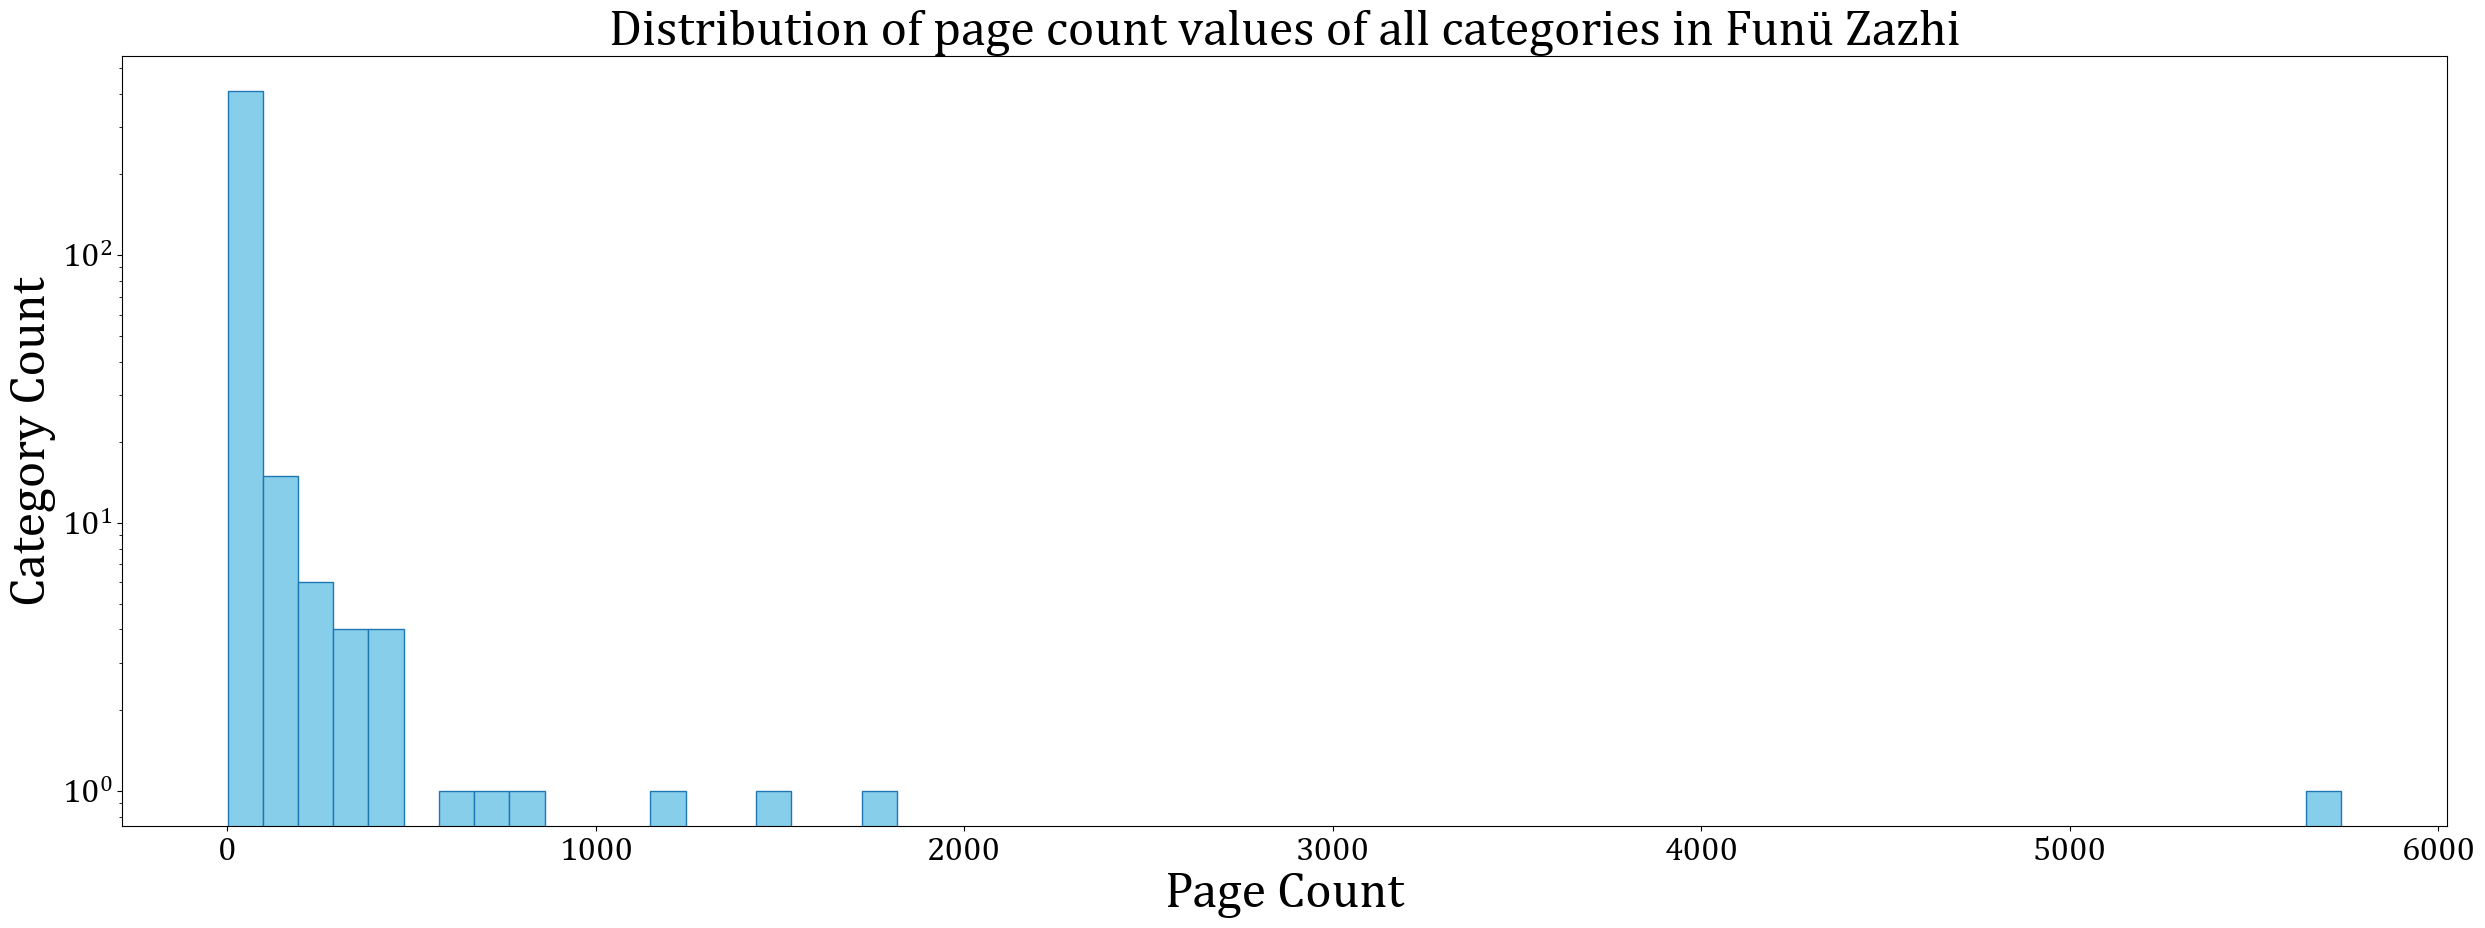
\includegraphics[width=\textwidth]{./figures/fnzz2}
    \caption{The distribution of page count of all categories (exclude undefined)}
    \label{fig:fnzz2}
\end{figure}

Figure \ref{fig:fnzz3} shows sample images of 4 categories in Funü Zazhi, where the text layout is different and the image quality varies. However, around 80\% of images have a text layout similar to Figure \ref{fig:fnzz3.2}, where the text is divided into the upper and lower parts, and for each part it reads vertically from right to left. The rest of the images have different text layouts, such as the one in Figure \ref{fig:fnzz3.3}, where it contains both horizontal and vertical text.

\begin{figure}[htbp]
    \centering
    \begin{subfigure}[b]{0.23\linewidth}
        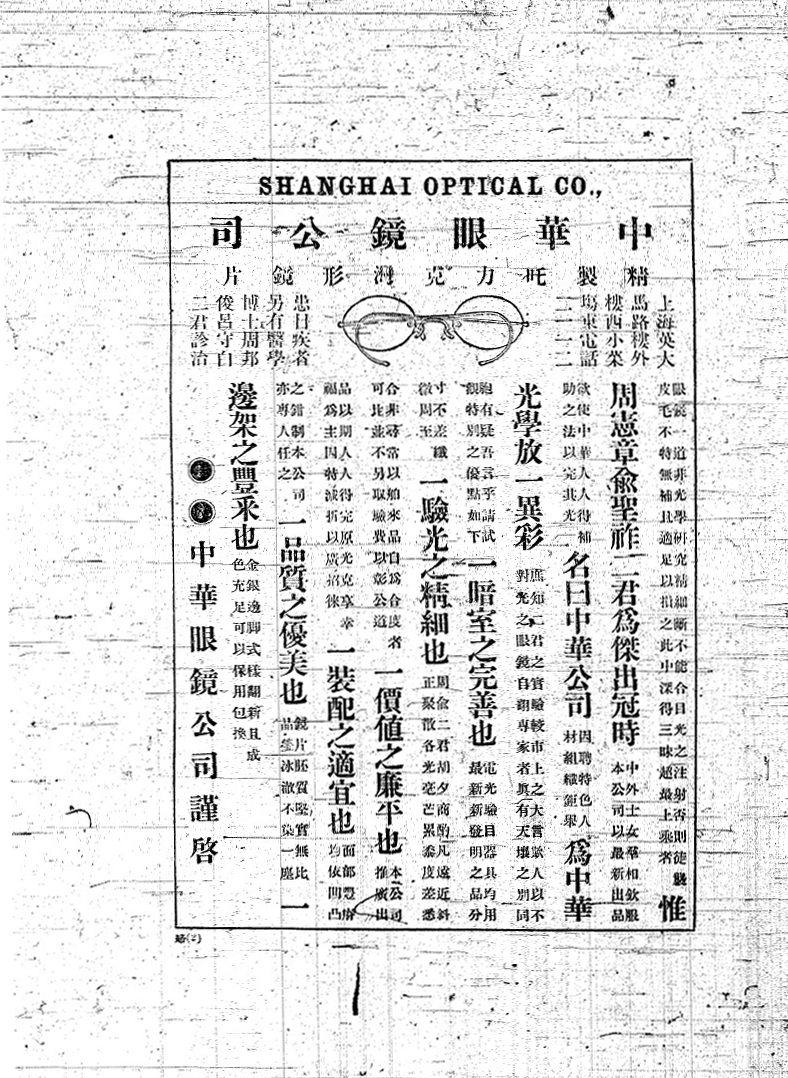
\includegraphics[width=\linewidth]{./figures/fnzz3.1}
        \caption{Advertisement}
        \label{fig:fnzz3.1}
    \end{subfigure}
    \hfill
    \begin{subfigure}[b]{0.23\linewidth}
        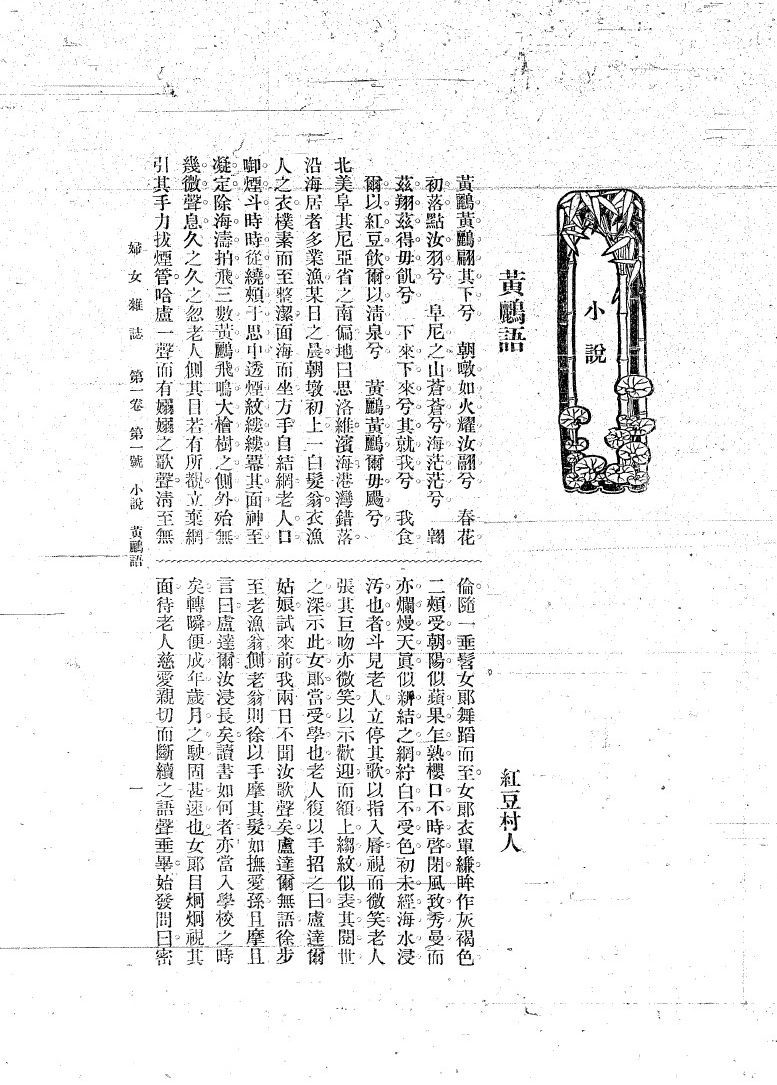
\includegraphics[width=\linewidth]{./figures/fnzz3.2}
        \caption{Novel}
        \label{fig:fnzz3.2}
    \end{subfigure}
    \hfill
    \begin{subfigure}[b]{0.23\linewidth}
        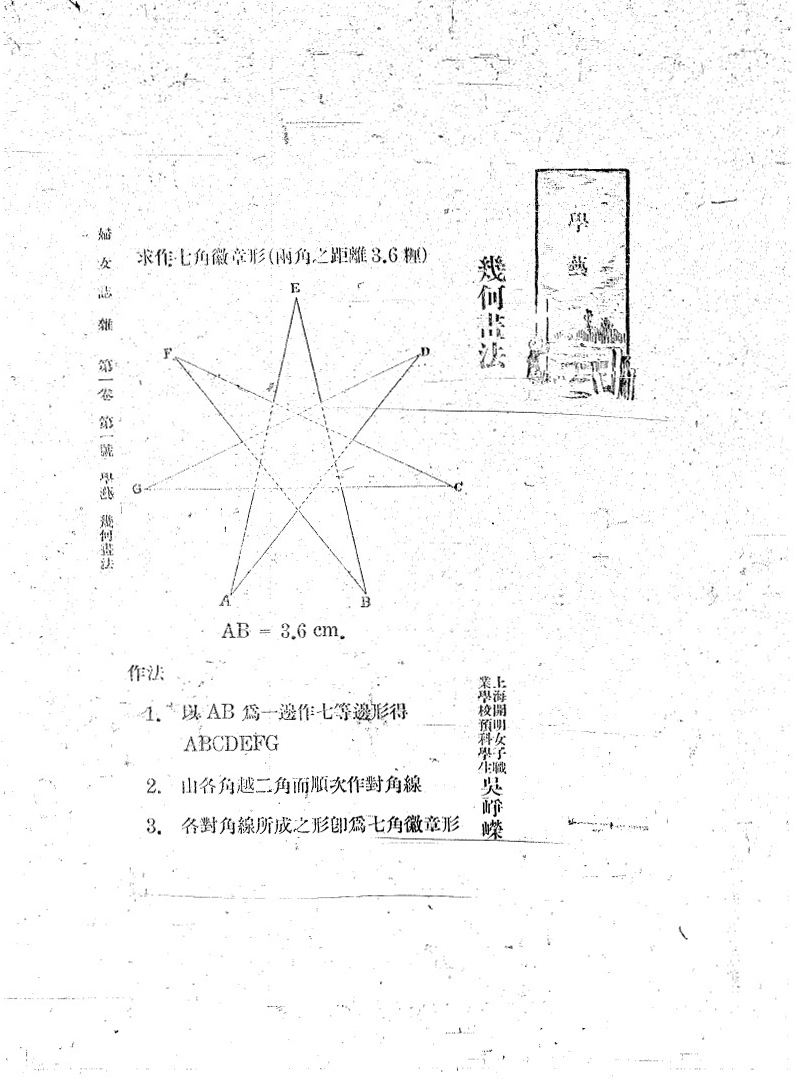
\includegraphics[width=\linewidth]{./figures/fnzz3.3}
        \caption{Study}
        \label{fig:fnzz3.3}
    \end{subfigure}
    \hfill
    \begin{subfigure}[b]{0.23\linewidth}
        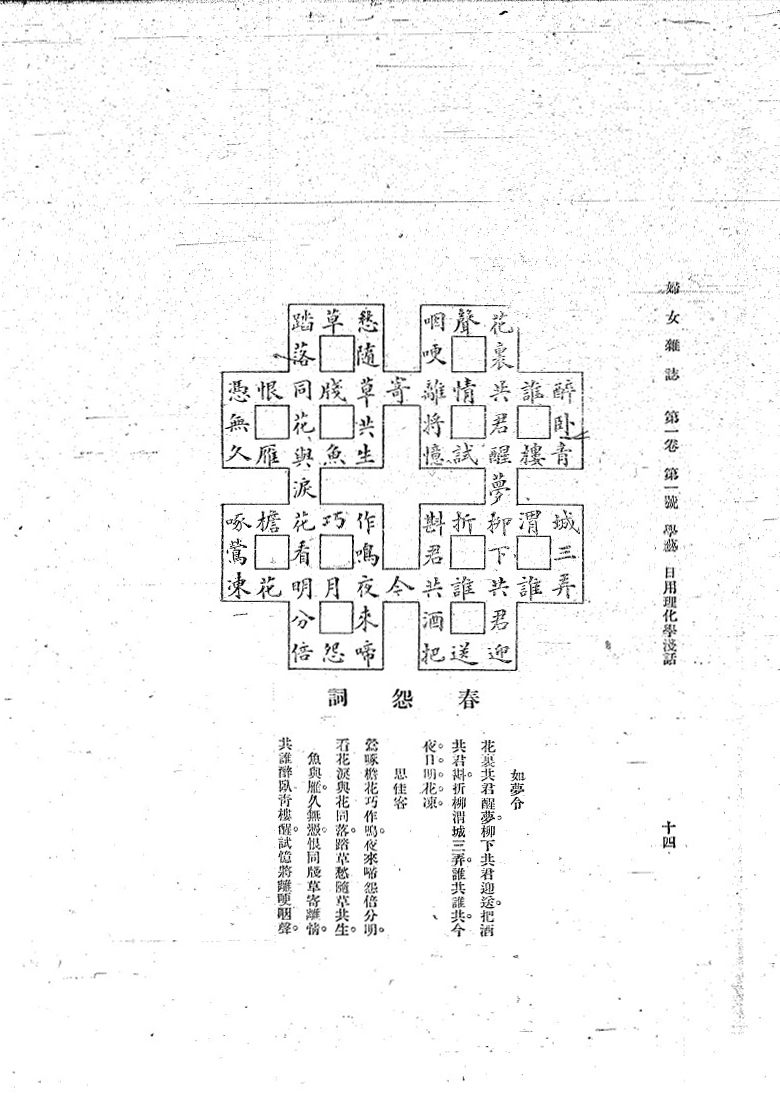
\includegraphics[width=\linewidth]{./figures/fnzz3.4}
        \caption{Filler}
        \label{fig:fnzz3.4}
    \end{subfigure}
    \caption{Sample images of 4 categories in Funü Zazhi}
    \label{fig:fnzz3}
\end{figure}

The images are downloaded from the database \cite{fnzzpages} and labeled by their issue and page number. For example, Figure \ref{fig:fnzz3.1} is labeled as ``1501\_0011.jpg", which means it is the 11th page of the January 1915 issue. The number of pages in each month is relatively stable during 1915 to 1922, but fluctuates significantly since 1922, as shown in Figure \ref{fig:fnzz4}. Most of the issues have less than 200 pages, but some issues have more than 300 pages. The lowest page count is 130 in the March 1921 issue, and the highest page count is 357 in the January 1925 issue.

\begin{figure}[htbp]
    \centering
    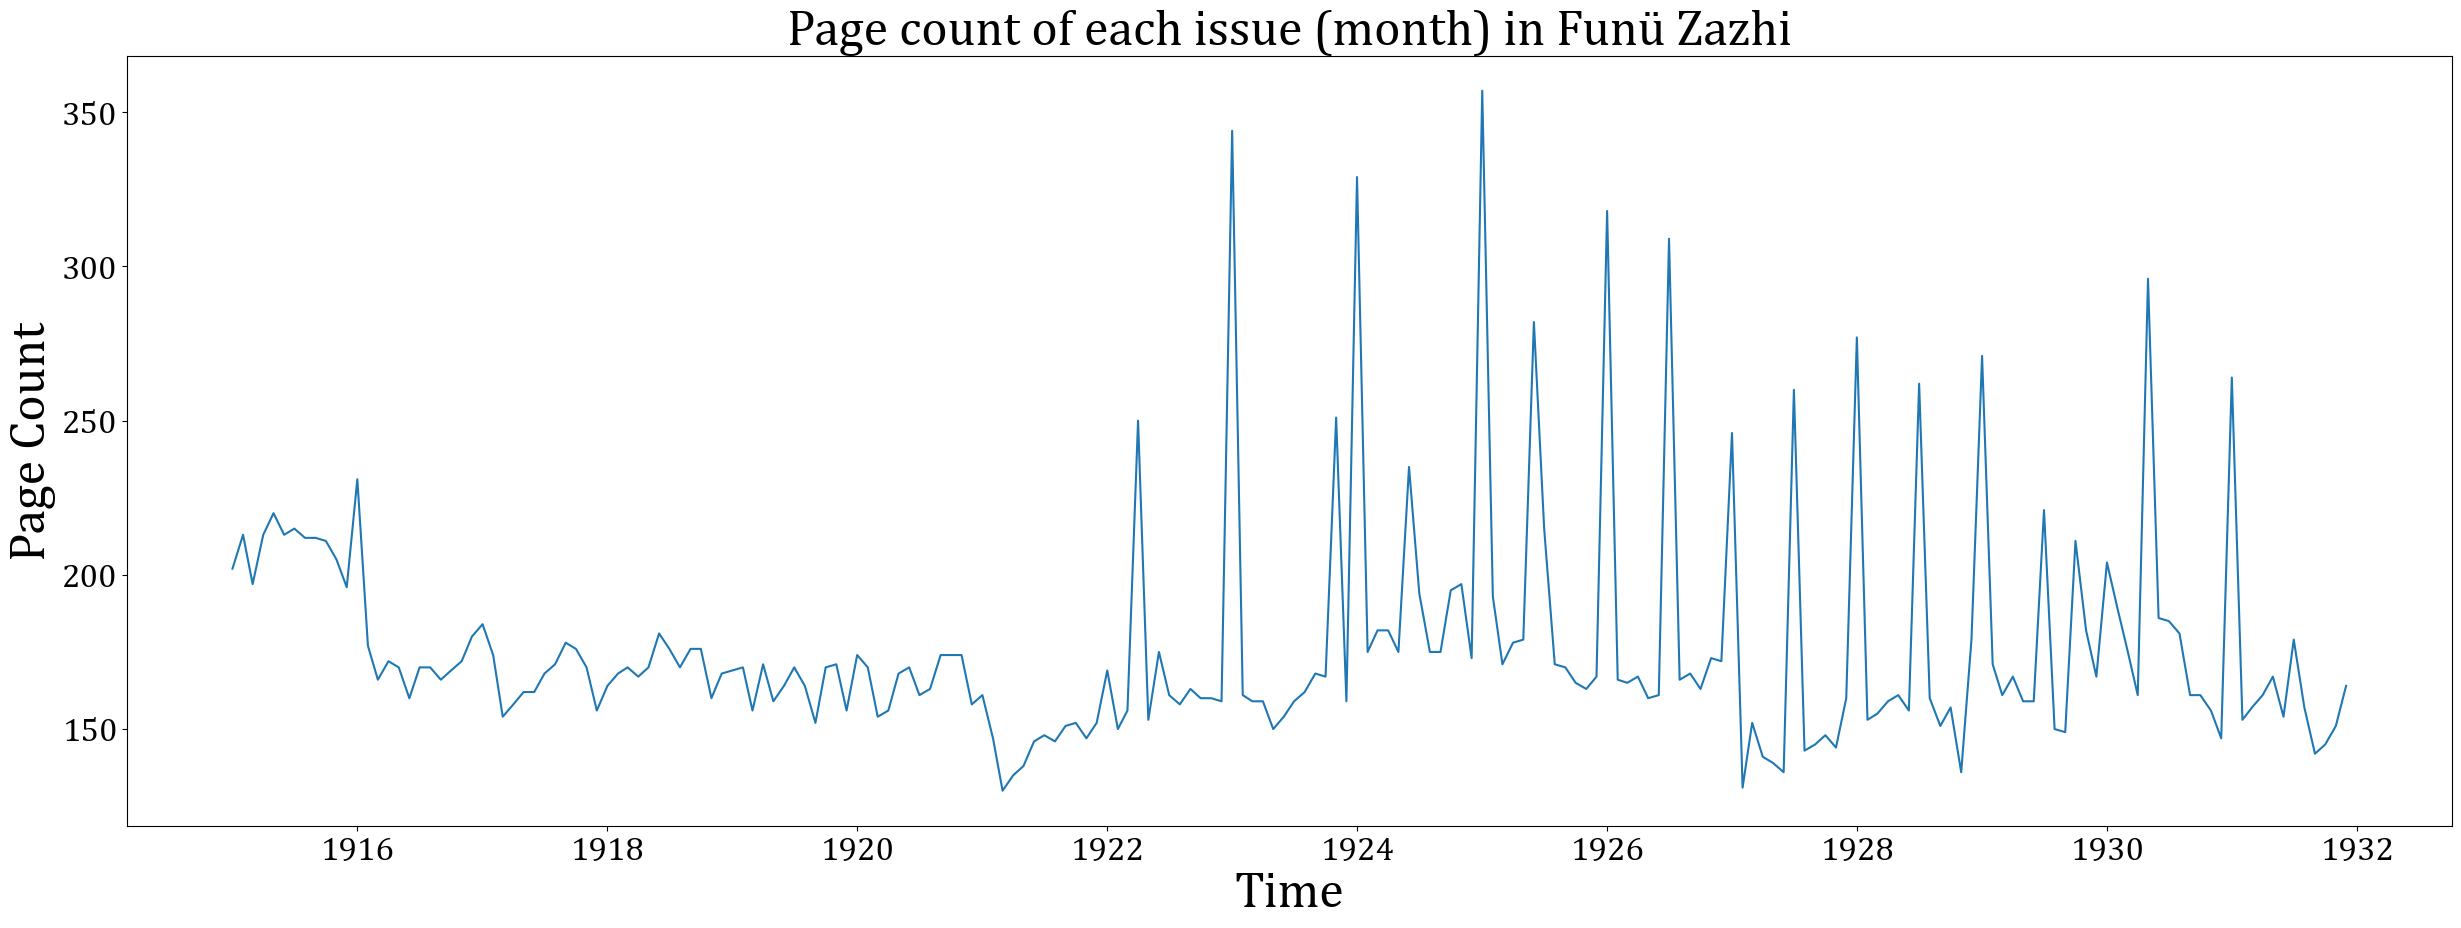
\includegraphics[width=\textwidth]{./figures/fnzz4}
    \caption{The number of pages by each issue (month) in Funü Zazhi}
    \label{fig:fnzz4}
\end{figure}

\section{System Overview}
\label{sec:system_overview}
The OCR system consists of three main components: text detection, text recognition, and text ordering, as shown in Figure \ref{fig:ocr_system}. The system takes images as input and outputs their text content with sensible order. The text detection module locates text line regions, extracting images of these regions and send them to the recognition module. The recognition module recognizes the content in the text lines, and the ordering module orders the text lines based on their positions given by the detection module. The final output combines the ordering and the recognition results, which gives the ordered text content in the image.

\begin{figure}[htbp]
    \centering
    \begin{tikzpicture}[node distance=5cm, auto, thick, scale=0.8, transform shape]
        % Define block styles
        \tikzstyle{block} = [rectangle, draw, fill=blue!20, text width=9em, text centered, rounded corners, minimum height=3em]

        % Place nodes
        \node [block, fill=red!20] (image) {Image};
        \node [block, right of=image] (text_detection) {Text Detection};
        \node [block, right of=text_detection, yshift=2cm] (text_recognition) {Text Recognition};
        \node [block, right of=text_detection, yshift=-2cm] (text_ordering) {Text Ordering};
        \node [block, fill=green!20, right of=text_ordering, yshift=2cm] (text) {Text};

        % Draw connections as arrows
        \draw [->] (image) -- (text_detection);
        \draw [->] (text_detection) -- (text_recognition);
        \draw [->] (text_detection) -- (text_ordering);
        \draw [->] (text_recognition) -- (text);
        \draw [->] (text_ordering) -- (text);

        % Add text on the arrows
        \node[align=center] at ($(text_detection)!0.5!(text_recognition)$) {\small Text line images};
        \node[align=center] at ($(text_detection)!0.5!(text_ordering)$) {\small Text line positions};
        \node[align=center] at ($(text_recognition)!0.5!(text)$) {\small Text line content};
        \node[align=center] at ($(text_ordering)!0.5!(text)$) {\small Text line order};
    \end{tikzpicture}
    \caption{Overall structure of the OCR system for Funü Zazhi}
    \label{fig:ocr_system}
\end{figure}

The architecture of the OCR system follows a traditional two-stage pipeline, where both text detection and recognition use deep learning models and are trained separately. Due to the lack of annotated dataset with similar characteristics to the target images, synthetic data will be used for training. The ordering method is rule-based, which does not require training. There are several reasons that two-stage method is adopted rather than end-to-end method:

\textbf{Design Flexibility}: Two-stage method allows for more flexibility in model design. More specialized models can be used for each task, utilizing the strengths of different architectures.

\textbf{Data Efficiency}: Two-stage methods can leverage different training data more effectively, and the combination of two types of synthetic data can better match the characteristics of the target images.

\textbf{Separate Optimization}: Text detection and recognition models can be trained without being influenced by each other's performance. This allows for more refined hyperparameter tuning and optimization.

\textbf{Variation Robustness}: Two-stage methods can better handle varied and complex text scenarios in Funü Zazhi, such as different text layout and backgrounds, by first isolating text regions before applying recognition algorithms.

\textbf{Component Modularity}: The system can be easily extended by replacing or updating individual components. Problems can be isolated and solved independently, which is beneficial for debugging and maintenance.

In general, while end-to-end OCR systems can be simpler and faster due to the unified approach, two-stage methods offer more flexibility, robustness and maintainability, which is crucial for handling the complex text scenarios in Funü Zazhi.

\section{Alternative Designs}
\label{sec:alternative_designs}
In the early stage of the project, several alternative designs were considered for the OCR system. However, they were not adopted due to complexity or performance. In addition to the line-level detection and recognition method described in Section \ref{sec:system_overview}, the following designs were experimented, but proved to be less efficient or robust:

\textbf{Character Detection and Classification}: This method detects, classifies and orders each character individually. The detection result as images of single characters will be sent to a character classifier, and the classification result will be ordered based on character's detected position. However, it struggled with detecting a large amount of characters in a single image.

\textbf{Character Recognition}: This method outputs the label and position of each character in a single forward pass, and then orders the labels based on their position, which is more efficient than the above method. However, it also struggled with detecting large amount of characters in a single image, and the recognition performance was not as good as the two-stage method.

\textbf{Textline Detection and Character Recognition}: This method first detects textline regions, then recognizes and orders characters in each region. The difference to our final design is in the recognition part, where it first outputs the recognized characters with their positions, and then orders them based on the position. However in our final design, the recognition part outputs the ordered text content in a text line directly, which is more efficient and robust.

The following diagram illustrates the structure of the alternative designs:

\begin{figure}[htbp]
    \centering
    \begin{tikzpicture}[node distance=5cm, auto, thick, scale=0.8, transform shape]
        % Define block styles
        \tikzstyle{block} = [rectangle, draw, fill=blue!20, text width=9em, text centered, rounded corners, minimum height=3em]

        % Place nodes
        \node [block, fill=red!20] (image) {Image};
        \node [block, right of=image] (text_detection) {Character Detection};
        \node [block, right of=text_detection, yshift=2cm] (text_recognition) {Character Classification};
        \node [block, right of=text_detection, yshift=-2cm] (text_ordering) {Character Ordering};
        \node [block, fill=green!20, right of=text_ordering, yshift=2cm] (text) {Text};

        % Draw connections as arrows
        \draw [->] (image) -- (text_detection);
        \draw [->] (text_detection) -- (text_recognition);
        \draw [->] (text_detection) -- (text_ordering);
        \draw [->] (text_recognition) -- (text);
        \draw [->] (text_ordering) -- (text);

        % Add text on the arrows
        \node[align=center] at ($(text_detection)!0.5!(text_recognition)$) {\small Character images};
        \node[align=center] at ($(text_detection)!0.5!(text_ordering)$) {\small Character positions};
        \node[align=center] at ($(text_recognition)!0.5!(text)$) {\small Character labels};
        \node[align=center] at ($(text_ordering)!0.5!(text)$) {\small Character order};

        % Add subtitles to the picture
        \node[align=center, yshift=2.5cm, xshift=1.75cm] at (image) {\textbf{Character Detection and Classification}};

        % Leave some space for the next picture
        \node[align=center, yshift=-2cm] at (text_ordering) {};
    \end{tikzpicture}

    \begin{tikzpicture}[node distance=5cm, auto, thick, scale=0.8, transform shape]
        % Define block styles
        \tikzstyle{block} = [rectangle, draw, fill=blue!20, text width=9em, text centered, rounded corners, minimum height=3em]

        % Place nodes
        \node [block, fill=red!20] (image) {Image};
        \node [block, right of=image] (text_recognition) {Character Recognition};
        \node [block, right of=text_recognition, yshift=2cm] (text_ordering) {Character Ordering};
        \node [block, fill=green!20, right of=text_ordering, yshift=-2cm] (text) {Text};

        % Draw connections as arrows
        \draw [->] (image) -- (text_recognition);
        \draw [->] (text_recognition) -- (text_ordering);
        \draw [->] (text_recognition) -- (text);
        \draw [->] (text_ordering) -- (text);

        % Add text on the arrows
        \node[align=center, yshift=-0.4cm] at ($(text_recognition)!0.5!(text)$) {\small Character labels};
        \node[align=center] at ($(text_recognition)!0.5!(text_ordering)$) {\small Character positions};
        \node[align=center] at ($(text_ordering)!0.5!(text)$) {\small Character order};

        % Add subtitles to the picture
        \node[align=center, yshift=2.5cm, xshift=0.2cm] at (image) {\textbf{Character Recognition}};

        % Leave some space for the next picture
        \node[align=center, yshift=-2cm] at (text) {};
    \end{tikzpicture}

    \begin{tikzpicture}[node distance=5cm, auto, thick, scale=0.8, transform shape]
        % Define block styles
        \tikzstyle{block} = [rectangle, draw, fill=blue!20, text width=9em, text centered, rounded corners, minimum height=3em]

        % Place nodes
        \node [block, fill=red!20] (image) {Image};
        \node [block, right of=image] (text_detection) {Textline Detection};
        \node [block, right of=text_detection, yshift=3cm] (text_recognition) {Character Recognition};
        \node [block, right of=text_detection] (character_ordering) {Character Ordering};
        \node [block, right of=text_detection, yshift=-3cm] (text_ordering) {Textline Ordering};
        \node [block, fill=green!20, right of=character_ordering] (text) {Text};

        % Draw connections as arrows
        \draw [->] (image) -- (text_detection);
        \draw [->] (text_detection) -- (text_recognition);
        \draw [->] (text_detection) -- (text_ordering);
        \draw [->] (text_recognition) -- (character_ordering);
        \draw [->] (text_recognition) -- (text);
        \draw [->] (character_ordering) -- (text);
        \draw [->] (text_ordering) -- (text);

        % Add text on the arrows
        \node[align=center, xshift=-2cm] at ($(text_detection)!0.5!(text_recognition)$) {\small Text line images};
        \node[align=center, xshift=-2cm] at ($(text_detection)!0.5!(text_ordering)$) {\small Text line positions};
        \node[align=center] at ($(text_recognition)!0.5!(character_ordering)$) {\small Character positions};
        \node[align=center, xshift=2cm] at ($(text_recognition)!0.5!(text)$) {\small Character labels};
        \node[align=center, yshift=-1cm] at (character_ordering) {\small Character order in text lines};
        \node[align=center, xshift=2cm] at ($(text_ordering)!0.5!(text)$) {\small Text line order};

        % Add subtitles to the picture
        \node[align=center, yshift=3.5cm, xshift=2.45cm] at (image) {\textbf{Textline Detection and Character Recognition}};

        % Leave some space for the next picture
        \node[align=center, yshift=-1cm] at (text_ordering) {};
    \end{tikzpicture}
    \caption{Alternative designs of the OCR system}
    \label{fig:alt_ocr_system}
\end{figure}

%%%%%%%%%%%%%%%%%%%%%%%%%%%%%%%%%%%%
\chapter{Implementation}
This chapter describes the implementation details of the OCR system, the synthetic dataset, and the user interface.

\section{OCR System}
\label{sec:ocr_system}
The OCR system is implemented in Python, using PyTorch \cite{paszke2019pytorch} for deep learning models. As described in Section \ref{sec:system_overview}, the system consists of three main components: text detection, text recognition, and text ordering. Each component is implemented as a separate module, and they are combined to form the complete OCR system. While some alternative designs (Section \ref{sec:alternative_designs}) were implemented in early experiments, they will not be discussed in this section.

\subsection{Text Detection}
\label{sec:text_detection}
Considering the nature of the scanned document images as discussed in Section \ref{sec:target_dataset}, we treat the text detection task as an object detection problem, where the target is rectangular text lines. Therefore, regression-based methods are more suitable than segmentation-based approaches, as we can predict the bounding box of the text line directly, without the need to obtain a segmentation mask for irregular text regions.

The text detection model is based on the Faster R-CNN \cite{ren2015faster} architecture, a widely used object detection model, and often considered more accurate than single-stage models like YOLO \cite{redmon2016yolo9000} or SSD \cite{liu2016ssd}. The model's implementation in this project consists of a ResNet-50 FPN backbone \cite{he2015resnet,li2021benchmark} for initial feature extraction, a Region Proposal Network (RPN) \cite{ren2015faster} for generating text line proposals, and a Region of Interest (RoI) pooling layer \cite{ren2015faster} to extract fixed-size features from proposals, which are then fed into a classification and regression head to predict the label and bounding box of the target text line, as shown in Figure \ref{fig:faster_rcnn}.

In our design, there are three types of target labels, which are background, vertical text line, and horizontal text line. The background label is used to filter out non-text regions, while the vertical and horizontal text line labels indicate the orientation of the text line. In a tradition Chinese document like Funü Zazhi \cite{fnzz}, a vertical text line is not a 90-degree rotated horizontal text line, as the orientation of the characters is the same in both cases, but the reading direction is different. Therefore, we treat vertical and horizontal text lines as two separate categories, and the model is trained to distinguish between them.

\begin{figure}[htbp]
    \centering
    \begin{tikzpicture}[node distance=5cm, auto, thick, scale=0.8, transform shape]
        % Define block styles
        \tikzstyle{block} = [rectangle, draw, fill=blue!20, text width=9em, text centered, rounded corners, minimum height=3em]

        % Place nodes
        \node [block, fill=red!20] (image) {Image};
        \node [block, right of=image] (backbone) {ResNet-50 FPN Backbone};
        \node [block, right of=backbone, xshift=-2.5cm, yshift=3cm] (rpn) {Region Proposal Network};
        \node [block, right of=backbone] (roi) {Region of Interest Pooling};
        \node [block, right of=roi, xshift=-2.5cm, yshift=3cm] (cla_head) {Classification Head};
        \node [block, right of=roi, xshift=-2.5cm, yshift=-3cm] (reg_head) {Regression Head};
        \node [block, fill=green!20, right of=roi] (output) {Textline Bounding Boxes and Labels};

        % Draw connections as arrows
        \draw [->] (image) -- (backbone);
        \draw [->] (backbone) -- (rpn);
        \draw [->] (backbone) -- (roi);
        \draw [->] (rpn) -- (roi);
        \draw [->] (roi) -- (cla_head);
        \draw [->] (roi) -- (reg_head);
        \draw [->] (cla_head) -- (output);
        \draw [->] (reg_head) -- (output);

        % Add text on the arrows
        \node[align=center, xshift=-1cm] at ($(backbone)!0.5!(rpn)$) {\small Feature maps};
        \node[align=center, yshift=-1cm] at ($(backbone)!0.5!(roi)$) {\small Feature maps};
        \node[align=center, xshift=-0.5cm] at ($(rpn)!0.5!(roi)$) {\small Region proposals};
        \node[align=center, xshift=0.5cm] at ($(roi)!0.5!(cla_head)$) {\small Fixed-size features};
        \node[align=center] at ($(roi)!0.5!(reg_head)$) {\small Fixed-size features};
        \node[align=center, xshift=1.5cm] at ($(cla_head)!0.5!(output)$) {\small Text line labels};
        \node[align=center, xshift=1.5cm] at ($(reg_head)!0.5!(output)$) {\small Text line positions};

    \end{tikzpicture}
    \caption{Faster R-CNN architecture for text detection}
    \label{fig:faster_rcnn}
\end{figure}

The loss function for the text detection model is a combination of the classification loss and the regression loss. The classification loss is calculated using the Cross-Entropy loss \cite{crossentropyloss}, while the regression loss is calculated using the Smooth L1 loss \cite{smoothl1loss}. The total loss is the sum of the classification loss and the regression loss, weighted by a hyperparameter $\lambda$:
\begin{equation}
    \mathcal{L} = \mathcal{L}_{\text{cls}} + \lambda \mathcal{L}_{\text{reg}}
\end{equation}
Where the classification loss $\mathcal{L}_{\text{cls}}$ is defined as:
\begin{equation}
    \mathcal{L}_{\text{cls}} = -\frac{1}{N_{\text{cls}}} \sum_{i=1}^{N_{\text{cls}}} \left( y_i \log(\hat{y}_i) + (1 - y_i) \log(1 - \hat{y}_i) \right)
\end{equation}
Where $N_{\text{cls}}$ is the number of text line proposals, $y_i$ is the ground truth label of the $i$-th proposal, $\hat{y}_i$ is the predicted label of the $i$-th proposal, and the regression loss $\mathcal{L}_{\text{reg}}$ is defined as:
\begin{equation}
    \mathcal{L}_{\text{reg}} = \frac{1}{N_{\text{reg}}} \sum_{i=1}^{N_{\text{reg}}} \text{smooth}_{l_1}(t_i - \hat{t}_i)
\end{equation}
Where $N_{\text{reg}}$ is the number of positive text line proposals, $t_i$ is the ground truth bounding box of the $i$-th proposal, $\hat{t}_i$ is the predicted bounding box of the $i$-th proposal, and $\text{smooth}_{l_1}(x)$ is the Smooth L1 loss function:
\begin{equation}
    \text{smooth}_{l_1}(x) = \begin{cases}
        0.5 x^2 & \text{if } |x| < 1 \\
        |x| - 0.5 & \text{otherwise}
    \end{cases}
\end{equation}

\subsection{Text Recognition}
\label{sec:text_recognition}
The text recognition model is based on the CRNN \cite{shi2016end} architecture, a widely used CTC-based text recognition model. Considering the nature of Chinese text recognition, we choose CTC-based method rather than encoder-decoder method for the following reasons:

\textbf{Character Alignment}: Chinese characters in Funü Zazhi are often densely packed and have complex structures, unlike English words that are separated by spaces, making character alignment difficult. CTC-based methods can handle this issue by allowing the model to predict a sequence of characters without requiring each character to be aligned with specific image regions.

\textbf{Language Independence}: CTC-based methods are less language-dependent than encoder-decoder methods, as they do not require explicit language modeling. This is beneficial for recognizing the diverse content in Funü Zazhi, which includes a large character set and various language styles, such as classical and modern Chinese.

\textbf{Efficiency}: CTC-based methods are generally less computationally expensive than encoder-decoder methods, as they do not require the attention mechanism or recurrent connections between encoder and decoder. This can lead to easier training and faster inference, which benefits processing Chinese text with large character sets.

The CRNN \cite{shi2016end} model's implementation in this project consists of a Convolutional Neural Network (CNN) followed by a Recurrent Neural Network (RNN), as shown in Figure \ref{fig:crnn}. The CNN extracts visual features from the input text line image, which are then fed into a RNN with two stacked bidirectional Long Short-Term Memory (BiLSTM) to capture sequential dependencies and output predictions for each time step, corresponding to characters in the text line.

\begin{figure}[htbp]
    \centering
    \begin{tikzpicture}[node distance=5cm, auto, thick, scale=0.8, transform shape]
        % Define block styles
        \tikzstyle{block} = [rectangle, draw, fill=blue!20, text width=9em, text centered, rounded corners, minimum height=3em]
        \tikzstyle{smallblock} = [rectangle, draw, fill=blue!10, text width=8em, text centered, rounded corners, minimum height=1.5em]

        % Place main nodes
        \node [block, fill=red!20] (image) {Textline Image};
        \node [block, right of=image, minimum height=18em] (cnn) {};
        \node [block, right of=cnn, minimum height=11.5em] (rnn) {};
        \node [block, fill=green!20, right of=rnn] (output) {Textline Content};

        % Place small blocks inside CNN
        \node [smallblock, below=0.8cm of cnn.north] (conv1) {\tiny Conv1+ReLU+MaxPool};
        \node [smallblock, below=0.3cm of conv1] (conv2) {\tiny Conv2+ReLU+MaxPool};
        \node [smallblock, below=0.3cm of conv2] (conv3) {\tiny Conv3+BatchNorm+ReLU};
        \node [smallblock, below=0.3cm of conv3] (conv4) {\tiny Conv4+ReLU+MaxPool};
        \node [smallblock, below=0.3cm of conv4] (conv5) {\tiny Conv5+BatchNorm+ReLU};
        \node [smallblock, below=0.3cm of conv5] (conv6) {\tiny Conv6+ReLU+MaxPool};
        \node [smallblock, below=0.3cm of conv6] (conv7) {\tiny Conv7+BatchNorm+ReLU+AvgPool};

        % Place small blocks inside RNN
        \node [smallblock, below=0.8cm of rnn.north] (bilstm1) {\tiny BiLSTM1};
        \node [smallblock, below=0.3cm of bilstm1] (embed1) {\tiny Linear Embedding};
        \node [smallblock, below=0.3cm of embed1] (bilstm2) {\tiny BiLSTM2};
        \node [smallblock, below=0.3cm of bilstm2] (embed2) {\tiny Linear Embedding};

        % Draw connections as arrows
        \draw [->] (image) -- (cnn);
        \draw [->] (cnn) -- (rnn);
        \draw [->] (rnn) -- (output);

        % Draw connections within CNN
        \draw [->] (conv1) -- (conv2);
        \draw [->] (conv2) -- (conv3);
        \draw [->] (conv3) -- (conv4);
        \draw [->] (conv4) -- (conv5);
        \draw [->] (conv5) -- (conv6);
        \draw [->] (conv6) -- (conv7);

        % Draw connections within RNN
        \draw [->] (bilstm1) -- (embed1);
        \draw [->] (embed1) -- (bilstm2);
        \draw [->] (bilstm2) -- (embed2);

        % Add text on the arrows
        \node[align=center, yshift=3.4cm] at (cnn) {CNN};
        \node[align=center, yshift=2cm] at (rnn) {RNN};

    \end{tikzpicture}
    \caption{CRNN architecture for text recognition}
    \label{fig:crnn}
\end{figure}

The Connectionist Temporal Classification (CTC) loss \cite{ctcloss} is used to train the CRNN model, which is specifically designed for sequence-to-sequence problems where the alignment between input and output sequences is unknown. During training, the CTC loss calculates the difference between the predicted sequence and the ground truth sequence by:
\begin{equation}
    \mathcal{L}_{\text{CTC}} = -\log (p(y | x))
\end{equation}
Where $x$ is the input text line image, $y$ is the ground truth text content, and $p(y | x)$ is the probability of the ground truth sequence given the input image:
\begin{equation}
    p(y | x) = \sum_{\pi \in \mathcal{B}^{-1}(y)} p(\pi | x)
\end{equation}
Where $\sum_{\pi \in \mathcal{B}^{-1}(y)}$ is the sum over all possible alignments $\pi$ that can be mapped to the target sequence $y$, $p(\pi | x)$ is the probability of a specific alignment $\pi$, which is calculated as the product of the probabilities of each character (or blank) at each time step:
\begin{equation}
    p(\pi | x) = \prod_{t=1}^{T} p(\pi_t | x_t)
\end{equation}
Where $T$ is the number of time steps in the output sequence, and $p(\pi_t | x_t)$ is the probability of observing character $\pi_t$ at time step $t$ given the input sequence $x$.

\subsection{Text Ordering}
\label{sec:text_ordering}
The text ordering module is a rule-based method that orders the recognized text lines based on their positions in the image. Since most of the text layout in Funü Zazhi is similar to Figure \ref{fig:fnzz3.2}, where the text is divided into the upper and lower parts, and for each part it reads vertically from right to left, we proposed an efficient algorithm to order the text lines for this specific layout L1, as shown in Algorithm \ref{alg:ordering_l1}.

\begin{algorithm}[htbp]
    \caption{Text Ordering Algorithm for Layout L1}
    \begin{algorithmic}[1]
        \State \textbf{Input:} Text line positions $\{p_1, p_2, \ldots, p_n\}$, where $p_i = (x_i, y_i, x'_i, y'_i)$ with $(x_i, y_i)$ being top-left corner and $(x'_i, y'_i)$ being bottom-right corner ($x_i < x'_i$ and $y_i < y'_i$)
        \State \textbf{Output:} Ordered text line positions $\{o_1, o_2, \ldots, o_n\}$
        \Function{OrderingL1}{$P=\{p_1, p_2, \ldots, p_n\}$}
            \State $y_{\text{min}} \gets \min \{y_i | i = 1, 2, \ldots, n\}$
            \State $y_{\text{max}} \gets \max \{y'_i | i = 1, 2, \ldots, n\}$
            \State $y_{\text{center}} \gets (y_{\text{min}}+y_{\text{max}})/2$
            \State $P_{\text{upper}} \gets \{p_i | i = 1, 2, \ldots, n \And (y_i+y'_i)/2 < y_{\text{center}}\}$
            \State $P_{\text{lower}} \gets \{p_i | i = 1, 2, \ldots, n \And (y_i+y'_i)/2 \geq y_{\text{center}}\}$
            \State $P_{\text{upper}} \gets \text{sort}(P_{\text{upper}}, \text{key}=\lambda p: p[0] + p[2], \text{reverse}=True)$
            \State $P_{\text{lower}} \gets \text{sort}(P_{\text{lower}}, \text{key}=\lambda p: p[0] + p[2], \text{reverse}=True)$
            \State \Return $P_{\text{upper}} + P_{\text{lower}}$
        \EndFunction
    \end{algorithmic}
    \label{alg:ordering_l1}
\end{algorithm}

The algorithm first calculates the minimum and maximum $y$-coordinates of the text line positions, taking their average as the $y$-coordinate of a ``central line" in the image, and then dividing the text lines into upper and lower parts based on their relative position to the central line. The text lines in each part are then sorted based on their $x$-coordinates in descending order, and the final ordered positions are obtained by concatenating the upper and lower parts.

For other text layouts, such as the one in Figure \ref{fig:fnzz3.1}, where it contains both vertical and horizontal text, there are different ordering rules. Due to the minority and variety of these layouts in Funü Zazhi, we use a more general algorithm to handle them, as shown in Algorithm \ref{alg:ordering_l2}.

\begin{algorithm}[htbp]
    \caption{Text Ordering Algorithm for Layout L2}
    \begin{algorithmic}[1]
        \State \textbf{Input:} Text line positions $\{p_1, p_2, \ldots, p_n\}$ and labels $\{l_1, l_2, \ldots, l_n\}$, where $p_i = (x_i, y_i, x'_i, y'_i)$ with $(x_i, y_i)$ being top-left corner, $(x'_i, y'_i)$ being bottom-right corner ($x_i < x'_i$ and $y_i < y'_i$), and $l_i$ being the orientation label of the $i$-th text line
        \State \textbf{Output:} Ordered text line positions $\{o_1, o_2, \ldots, o_n\}$
        \Function{OrderingL2}{$P=\{p_1, p_2, \ldots, p_n\}$, $L=\{l_1, l_2, \ldots, l_n\}$}
            \State $P_{\text{vertical}} \gets \{p_i | i = 1, 2, \ldots, n \And l_i = \text{vertical}\}$
            \State $P_{\text{horizontal}} \gets \{p_i | i = 1, 2, \ldots, n \And l_i = \text{horizontal}\}$
            \State $P_{\text{vertical}} \gets \text{sort}(P_{\text{vertical}}, \text{key}=\lambda p: p[0] + p[2], \text{reverse}=True)$
            \State $P_{\text{horizontal}} \gets \text{sort}(P_{\text{horizontal}}, \text{key}=\lambda p: p[1] + p[3], \text{reverse}=False)$
            \State \Return $P_{\text{vertical}} + P_{\text{horizontal}}$
        \EndFunction
    \end{algorithmic}
    \label{alg:ordering_l2}
\end{algorithm}

The algorithm first separates the text lines into vertical and horizontal parts based on their orientation labels given by the text detector (Section \ref{sec:text_detection}), and then sorts the vertical text lines based on their $x$-coordinates in descending order, and the horizontal text lines based on their $y$-coordinates in ascending order. The final ordered positions are obtained by concatenating the vertical and horizontal parts. This algorithm follows a general reading rule for the remaining minor layouts (we call them L2) in Funü Zazhi, where vertical text lines are read from right to left, and horizontal text lines are read from top to bottom.

To distinguish between layout L1 and L2, we count the number of vertical text lines in the upper part and lower part of the image. If the number in both parts is greater than a threshold, we consider it as layout L1, otherwise as layout L2. The threshold is determined based on the total number of text lines in the image. Therefore, the complete text ordering algorithm for Funü Zazhi is a combination of Algorithm \ref{alg:ordering_l1} and Algorithm \ref{alg:ordering_l2}, as shown in Algorithm \ref{alg:ordering}.

\begin{algorithm}[htbp]
    \caption{Complete Text Ordering Algorithm for Funü Zazhi}
    \begin{algorithmic}[1]
        \State \textbf{Input:} Text line positions $\{p_1, p_2, \ldots, p_n\}$ and labels $\{l_1, l_2, \ldots, l_n\}$, where $p_i = (x_i, y_i, x'_i, y'_i)$ with $(x_i, y_i)$ being top-left corner, $(x'_i, y'_i)$ being bottom-right corner ($x_i < x'_i$ and $y_i < y'_i$), and $l_i$ being the orientation label of the $i$-th text line
        \State \textbf{Output:} Ordered text line positions $\{o_1, o_2, \ldots, o_n\}$
        \Function{Ordering}{$P=\{p_1, p_2, \ldots, p_n\}$, $L=\{l_1, l_2, \ldots, l_n\}$}
            \If{$n = 0 \text{ or } 1$}
                \State \Return $P$
            \Else
                \State $y_{\text{min}} \gets \min \{y_i | i = 1, 2, \ldots, n\}$
                \State $y_{\text{max}} \gets \max \{y'_i | i = 1, 2, \ldots, n\}$
                \State $y_{\text{center}} \gets (y_{\text{min}}+y_{\text{max}})/2$
                \State $n_{\text{vertical, upper}} \gets \sum_{i=1}^{n} \mathbbm{1}(l_i = \text{vertical} \And (y_i + y'_i)/2 < y_{\text{center}})$
                \State $n_{\text{vertical, lower}} \gets \sum_{i=1}^{n} \mathbbm{1}(l_i = \text{vertical} \And (y_i + y'_i)/2 \geq y_{\text{center}})$
                \State $ T \gets \lambda n$, where $\lambda \in (0, \frac{1}{2})$ 
                \If{$n_{\text{vertical, upper}} > T \And n_{\text{vertical, lower}} > T$}
                    \State \Return \textsc{OrderingL1}($P$)
                \Else
                    \State \Return \textsc{OrderingL2}($P$, $L$)
                \EndIf
            \EndIf
        \EndFunction
    \end{algorithmic}
    \label{alg:ordering}
\end{algorithm}

The reason for using two separate algorithms for text ordering instead of a single complex one is that around 80\% of the text layouts in Funü Zazhi is consistent (layout L1), while the remaining is diverse (layout L2). By first distinguishing between the two layouts and then applying the corresponding ordering algorithm, we simplifies the problem and improves the efficiency and robustness of the system. Using a more complex rule-based method or a learned model to predict the layout may introduce unnecessary complexity and lead to overfitting, as the text layouts in Funü Zazhi are not strictly defined, and it is difficult to collect sufficient training data to cover all possible variations. 

\section{Synthetic Dataset}
\label{sec:synthetic_dataset}
The most challenging part in this project is the lack of annotated data with similar characteristics to Funü Zazhi \cite{fnzzpages}, for training and evaluating the text detection and recognition models. Therefore, we created two synthetic datasets, one for each task, that simulate the distribution of the target dataset (Section \ref{sec:target_dataset}), such as the text layout, font style, and character set, while providing ground truth annotations. The synthetic datasets are generated using a combination of text rendering, image augmentation, and text layout simulation techniques, as described below.

\subsection{Data for Detection}
\label{sec:synthetic_detection}
The synthetic dataset for text detection simulates various text layouts in Funü Zazhi, including layout L1 and L2 as described in Section \ref{sec:text_ordering}. The dataset consists of images with text lines in different orientations, positions, sizes and fonts, and varying background noises, to cover the diversity in the target dataset. The ground truth annotations include the bounding boxes (4 numbers) of the text lines and their orientation labels, which are used to train the text detection model.

There are two main steps in the data generation process: text line rendering and text layout simulation. In text line rendering, for each text line, we first randomly select some characters from a traditional Chinese character set, which contains 6,000 most frequent characters from a Chinese Character Frequency List \cite{charlist}. Then, we randomly choose a font style from a set of 12 traditional Chinese fonts that are commonly used in Funü Zazhi, as shown in Figure \ref{fig:fonts}. The selected characters are then rendered onto a blank image using the chosen font style with random font size.

\begin{figure}[htbp]
    \centering
    \begin{subfigure}[b]{0.1\linewidth}
        
\includegraphics[width=\linewidth]{./figures/fonts/642_0.jpg}
        \caption{}
        \label{fig:fonts1}
    \end{subfigure}
    \hfill
    \begin{subfigure}[b]{0.1\linewidth}
        
\includegraphics[width=\linewidth]{./figures/fonts/642_1.jpg}
        \caption{}
        \label{fig:fonts2}
    \end{subfigure}
    \hfill
    \begin{subfigure}[b]{0.1\linewidth}
        
\includegraphics[width=\linewidth]{./figures/fonts/642_2.jpg}
        \caption{}
        \label{fig:fonts3}
    \end{subfigure}
    \hfill
    \begin{subfigure}[b]{0.1\linewidth}
        
\includegraphics[width=\linewidth]{./figures/fonts/642_3.jpg}
        \caption{}
        \label{fig:fonts4}
    \end{subfigure}
    \hfill
    \begin{subfigure}[b]{0.1\linewidth}
        
\includegraphics[width=\linewidth]{./figures/fonts/642_4.jpg}
        \caption{}
        \label{fig:fonts5}
    \end{subfigure}
    \hfill
    \begin{subfigure}[b]{0.1\linewidth}
        
\includegraphics[width=\linewidth]{./figures/fonts/642_5.jpg}
        \caption{}
        \label{fig:fonts6}
    \end{subfigure}

    \begin{subfigure}[b]{0.1\linewidth}
        
\includegraphics[width=\linewidth]{./figures/fonts/642_6.jpg}
        \caption{}
        \label{fig:fonts7}
    \end{subfigure}
    \hfill
    \begin{subfigure}[b]{0.1\linewidth}
        
\includegraphics[width=\linewidth]{./figures/fonts/642_7.jpg}
        \caption{}
        \label{fig:fonts8}
    \end{subfigure}
    \hfill
    \begin{subfigure}[b]{0.1\linewidth}
        
\includegraphics[width=\linewidth]{./figures/fonts/642_8.jpg}
        \caption{}
        \label{fig:fonts9}
    \end{subfigure}
    \hfill
    \begin{subfigure}[b]{0.1\linewidth}
        
\includegraphics[width=\linewidth]{./figures/fonts/642_9.jpg}
        \caption{}
        \label{fig:fonts10}
    \end{subfigure}
    \hfill
    \begin{subfigure}[b]{0.1\linewidth}
        
\includegraphics[width=\linewidth]{./figures/fonts/642_10.jpg}
        \caption{}
        \label{fig:fonts11}
    \end{subfigure}
    \hfill
    \begin{subfigure}[b]{0.1\linewidth}
        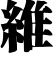
\includegraphics[width=\linewidth]{./figures/fonts/642_11.jpg}
        \caption{}
        \label{fig:fonts12}
    \end{subfigure}
    \caption{12 font styles of a specific traditional Chinese character. The corresponding typeface are: (a) Huawen Zhongsong, (b) Laobao Song, (c) Songti SC, (d) Songti, (e) Fangsong, (f) Kaiti, (g) Yuanyun Mingti, (h) Yuanxiang Mingti, (i) Yuanliu Mingti, (j) Jinghualao Songti, (k) Huiwen Mingti, (l) Xiangcuike Song}
    \label{fig:fonts}
\end{figure}

After rendering the text lines, we simulate the text layout by placing the text lines in different orientations and positions on the image. For layout L1, we divide the image into upper and lower parts, and place vertical text lines in each part, as shown in Figure \ref{fig:synthetic_det1}, where the bounding box for each text line is shown in red. We use the same typeface and font size for all text lines in one image, as the font style is consistent within a single page of Funü Zazhi for layout L1. The spacing between text lines is based on the font size, and the text line begins from the same y-coordinate in each part. Random transformation and noise is applied to the image afterwards to further increase the variety of synthetic data, including:

\begin{figure}[htbp]
    \centering
    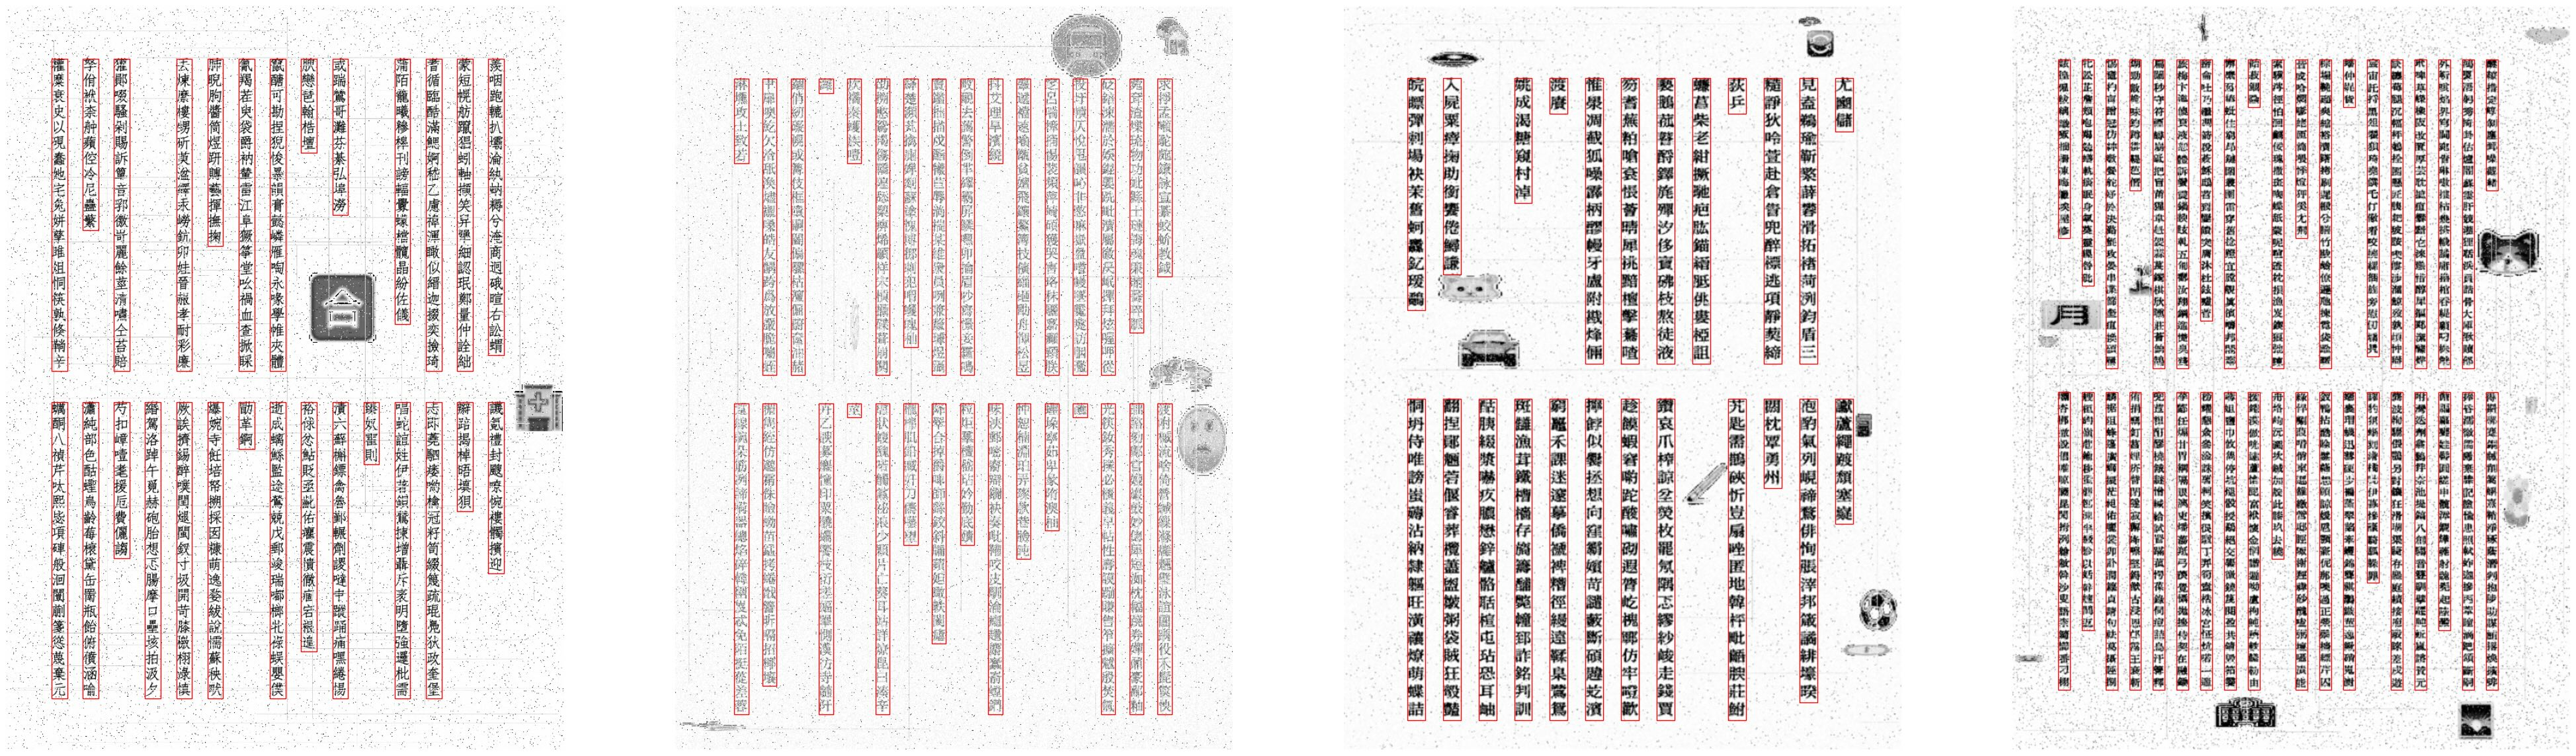
\includegraphics[width=\textwidth]{./figures/synthetic_det1.jpeg}
    \caption{Sample synthetic images in L1 for text detection with visualized annotations}
    \label{fig:synthetic_det1}
\end{figure}

\textbf{Image Rotation}: Randomly rotate the image by a small angle to simulate the skewness of the scanned document.

\textbf{Character Intensity Shift}: Randomly adjust the intensity of all characters in the image to simulate the effect of scanning or printing that may cause the characters to be lighter or darker.

\textbf{Background Noise}: Randomly add noise to the background of the image to simulate various noise in the scanned document, such as dust, scratches, or paper texture. Noise type includes Gaussian noise, salt-and-pepper noise, line-shaped noise, and erasing parts of the image. The intensity of each noise type is randomly selected.

\textbf{Non-text Elements}: Randomly select a few items from Icons-50 dataset \cite{icons50}, resize with different width and height, and overlay them on the synthetic image to simulate non-text elements in the scanned document, such as images and decorations.

For layout L2, due to the diversity, we randomly place the text lines with a mixture of vertical and horizontal orientations, as shown in Figure \ref{fig:synthetic_det2}, where the bounding box of vertical lines is shown in red and horizontal lines in green. The typeface and font size are randomly selected for each text line, as the font style can vary within a single page of Funü Zazhi for layout L2. The text lines can start from different positions with different spacing to each other. The same augmentation is applied to the image as in layout L1, and we randomly add a few blank between characters in some text lines to simulate various character spacing in the target dataset.

\begin{figure}[htbp]
    \centering
    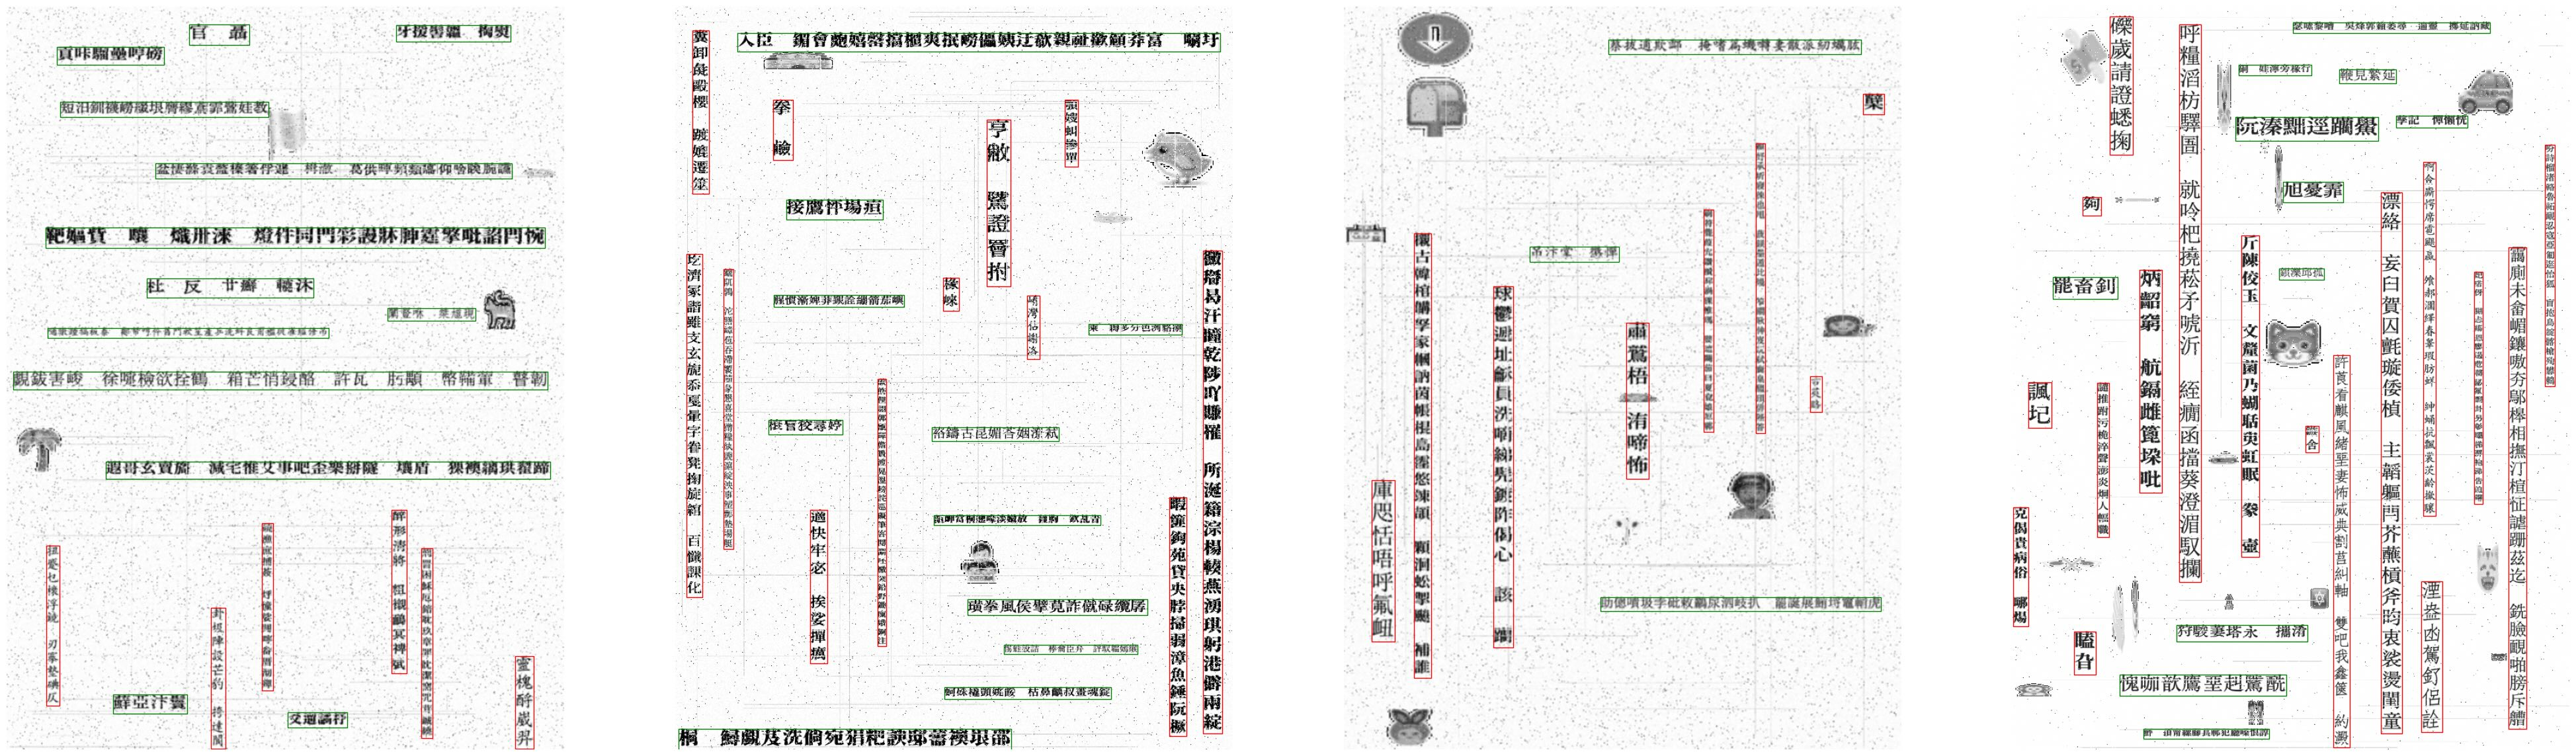
\includegraphics[width=\textwidth]{./figures/synthetic_det2.jpeg}
    \caption{Sample synthetic images in L2 for text detection with visualized annotations}
    \label{fig:synthetic_det2}
\end{figure}

The synthetic image is generated continuously during the training process, where in each iteration there will be a new batch of training data. This allows the model to see a wide variety of text layouts and background noises, which helps it generalize better to the target dataset. The proportion of layout L1 and L2 in the synthetic dataset is controlled by a hyperparameter $\alpha$. The complete hyperparameter settings for the text detection dataset generation is discussed in Section \ref{sec:text_detection_training}.

\subsection{Data for Recognition}
\label{sec:synthetic_recognition}
The synthetic dataset for text recognition simulates single text lines in Funü Zazhi. The dataset consists of images of text lines with varying orientations, font styles, sizes, and background noises, to cover the diversity in the target dataset. The ground truth annotation is the text content (character labels) of each text line, which is used to train the text recognition model.

The data generation process for text recognition is similar to the first step of text detection (Section \ref{sec:synthetic_detection}), where we render text lines with random characters, font styles and sizes, as shown in Figure \ref{fig:synthetic_rec}, while keeping the same typeface and font size within a single text line image. We use a mixture of vertical and horizontal text lines controlled by a proportion hyperparameter $\beta$. Random transformation and noise is applied to the image afterwards to further increase the variety, using the same augmentation techniques as discussed in Section \ref{sec:synthetic_detection}.

\begin{figure}[htbp]
    \centering
    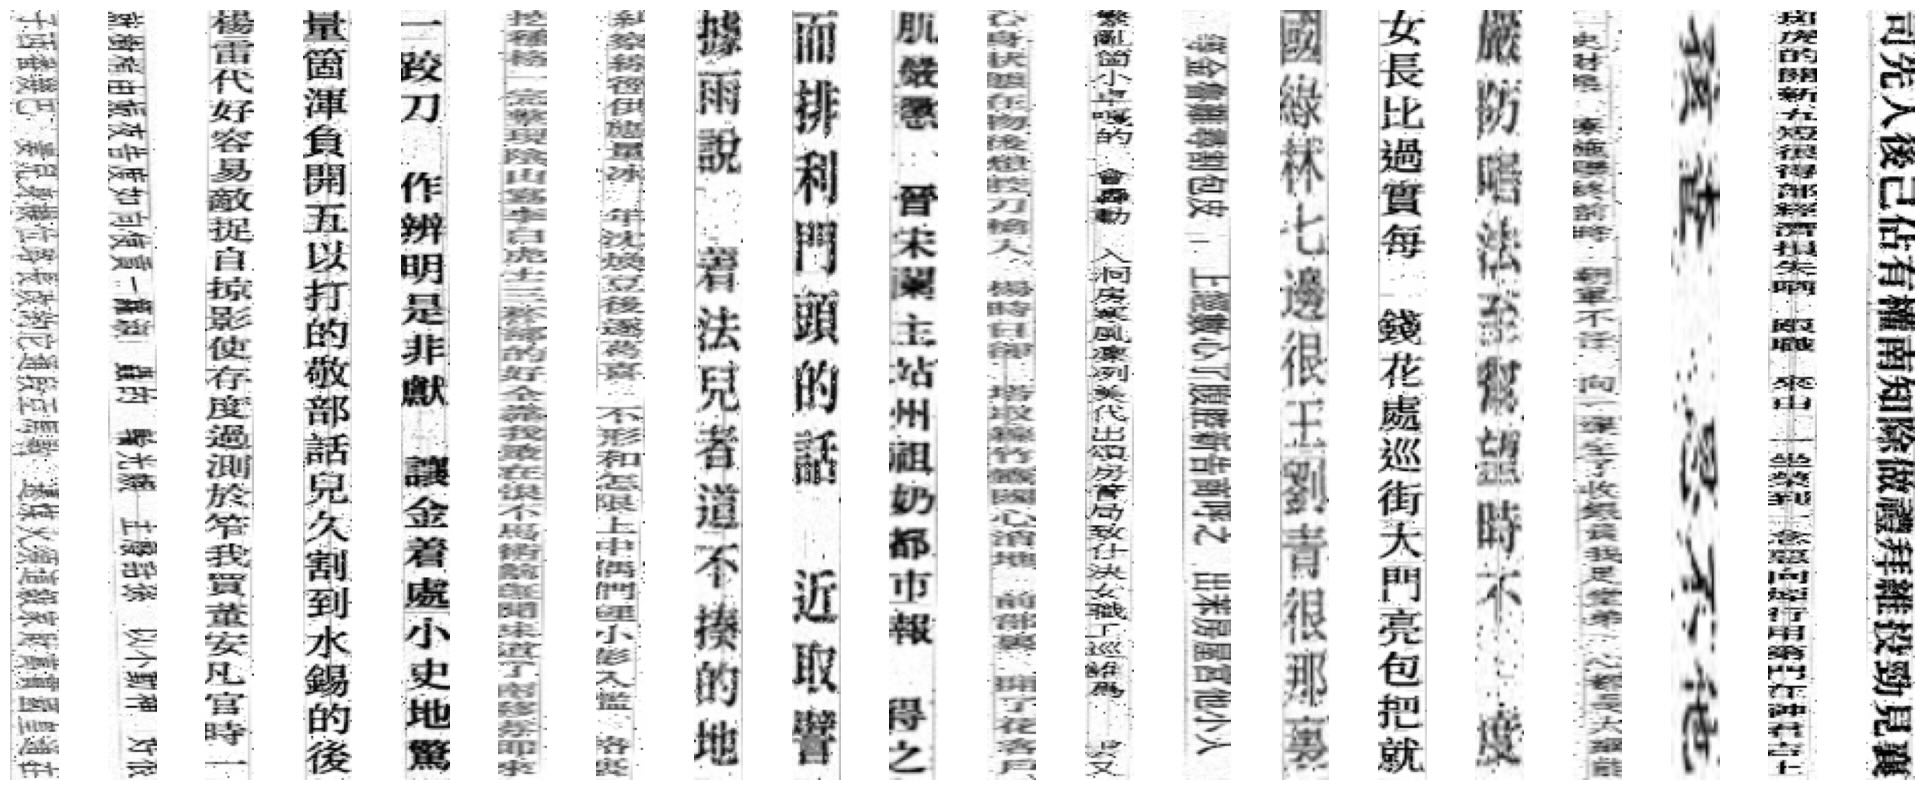
\includegraphics[width=\textwidth]{./figures/synthetic_rec.jpeg}
    \caption{Sample synthetic images for text recognition (horizontal lines are rotated)}
    \label{fig:synthetic_rec}
\end{figure}

To make the content in each text line more meaningful while preserving the diversity, we use the following techniques to select characters for rendering:

\textbf{Character Frequency}: Randomly select characters based on their frequency in a Character Frequency List \cite{charlist}, where more frequent characters are more likely to be selected. This helps to simulate the distribution of characters in the target dataset.

\textbf{Word Replacement}: Randomly replace some characters in a text line with common Chinese words or phrases from a database of 176,032 word vectors pre-trained with literature corpus \cite{wordlist}. This can generate text lines that capture word-level semantics in Funü Zazhi, and help the model learn the relationship between characters.

The text line rendering process firstly selects a random number of characters based on their frequency, and then replaces some characters with words or phrases based on a probability hyperparameter $\gamma$. The complete hyperparameter settings for the text recognition dataset generation is discussed in Section \ref{sec:text_recognition_training}.

\section{User Interface}
\label{sec:user_interface}
The user interface for the OCR system is implemented using the \texttt{tkinter} library, a standard GUI toolkit for Python. It is designed to be simple and intuitive, allowing users to easily upload scanned images of Funü Zazhi pages and receive the extracted text content in a sensible order. The interface consists of three main components: the image display area, the text content area, and some buttons and checkboxes, as shown in Figure \ref{fig:ui1.1}. The image display area will show the selected image once it is uploaded (Figure \ref{fig:ui1.2}), and the text content area will demonstrate the extracted text once the recognition process is completed, with the bounding boxes of text lines highlighted in the image display area (Figure \ref{fig:ui1.3}). The buttons and checkboxes allow users to upload images and extract text with different options, such as:

\textbf{Display Textline References}: Display the reference numbers of text lines in the text content area, which correspond to the order of text lines shown as small digits near the bounding boxes in the image display area (Figure \ref{fig:ui1.4}). This helps users to match the text content with the text lines in the image.

\textbf{Display Simplified Chinese}: Display the simplified Chinese characters of the extracted text content (Figure \ref{fig:ui1.5}). This is useful for users who are more familiar with simplified Chinese, as Funü Zazhi is written in traditional Chinese.

\textbf{Zoom and Shift Image}: When using the mouse wheel (or trackpad gestures) on the image display area, the image can be zoomed in or out, and when dragging the image, it can be shifted to view its different parts (Figure \ref{fig:ui1.6}). This helps users to inspect the text lines more closely and navigate through large images.

Once the text is recognized, a confidence score from 0 to 1 is displayed at the top of the interface, indicating the estimated accuracy of the recognition result, as discussed in Section \ref{sec:confidence_score}. This allows users to evaluate the quality of the extracted text and decide whether to make corrections or adjustments.

\begin{figure}[htbp]
    \centering
    \begin{subfigure}[b]{0.3\linewidth}
        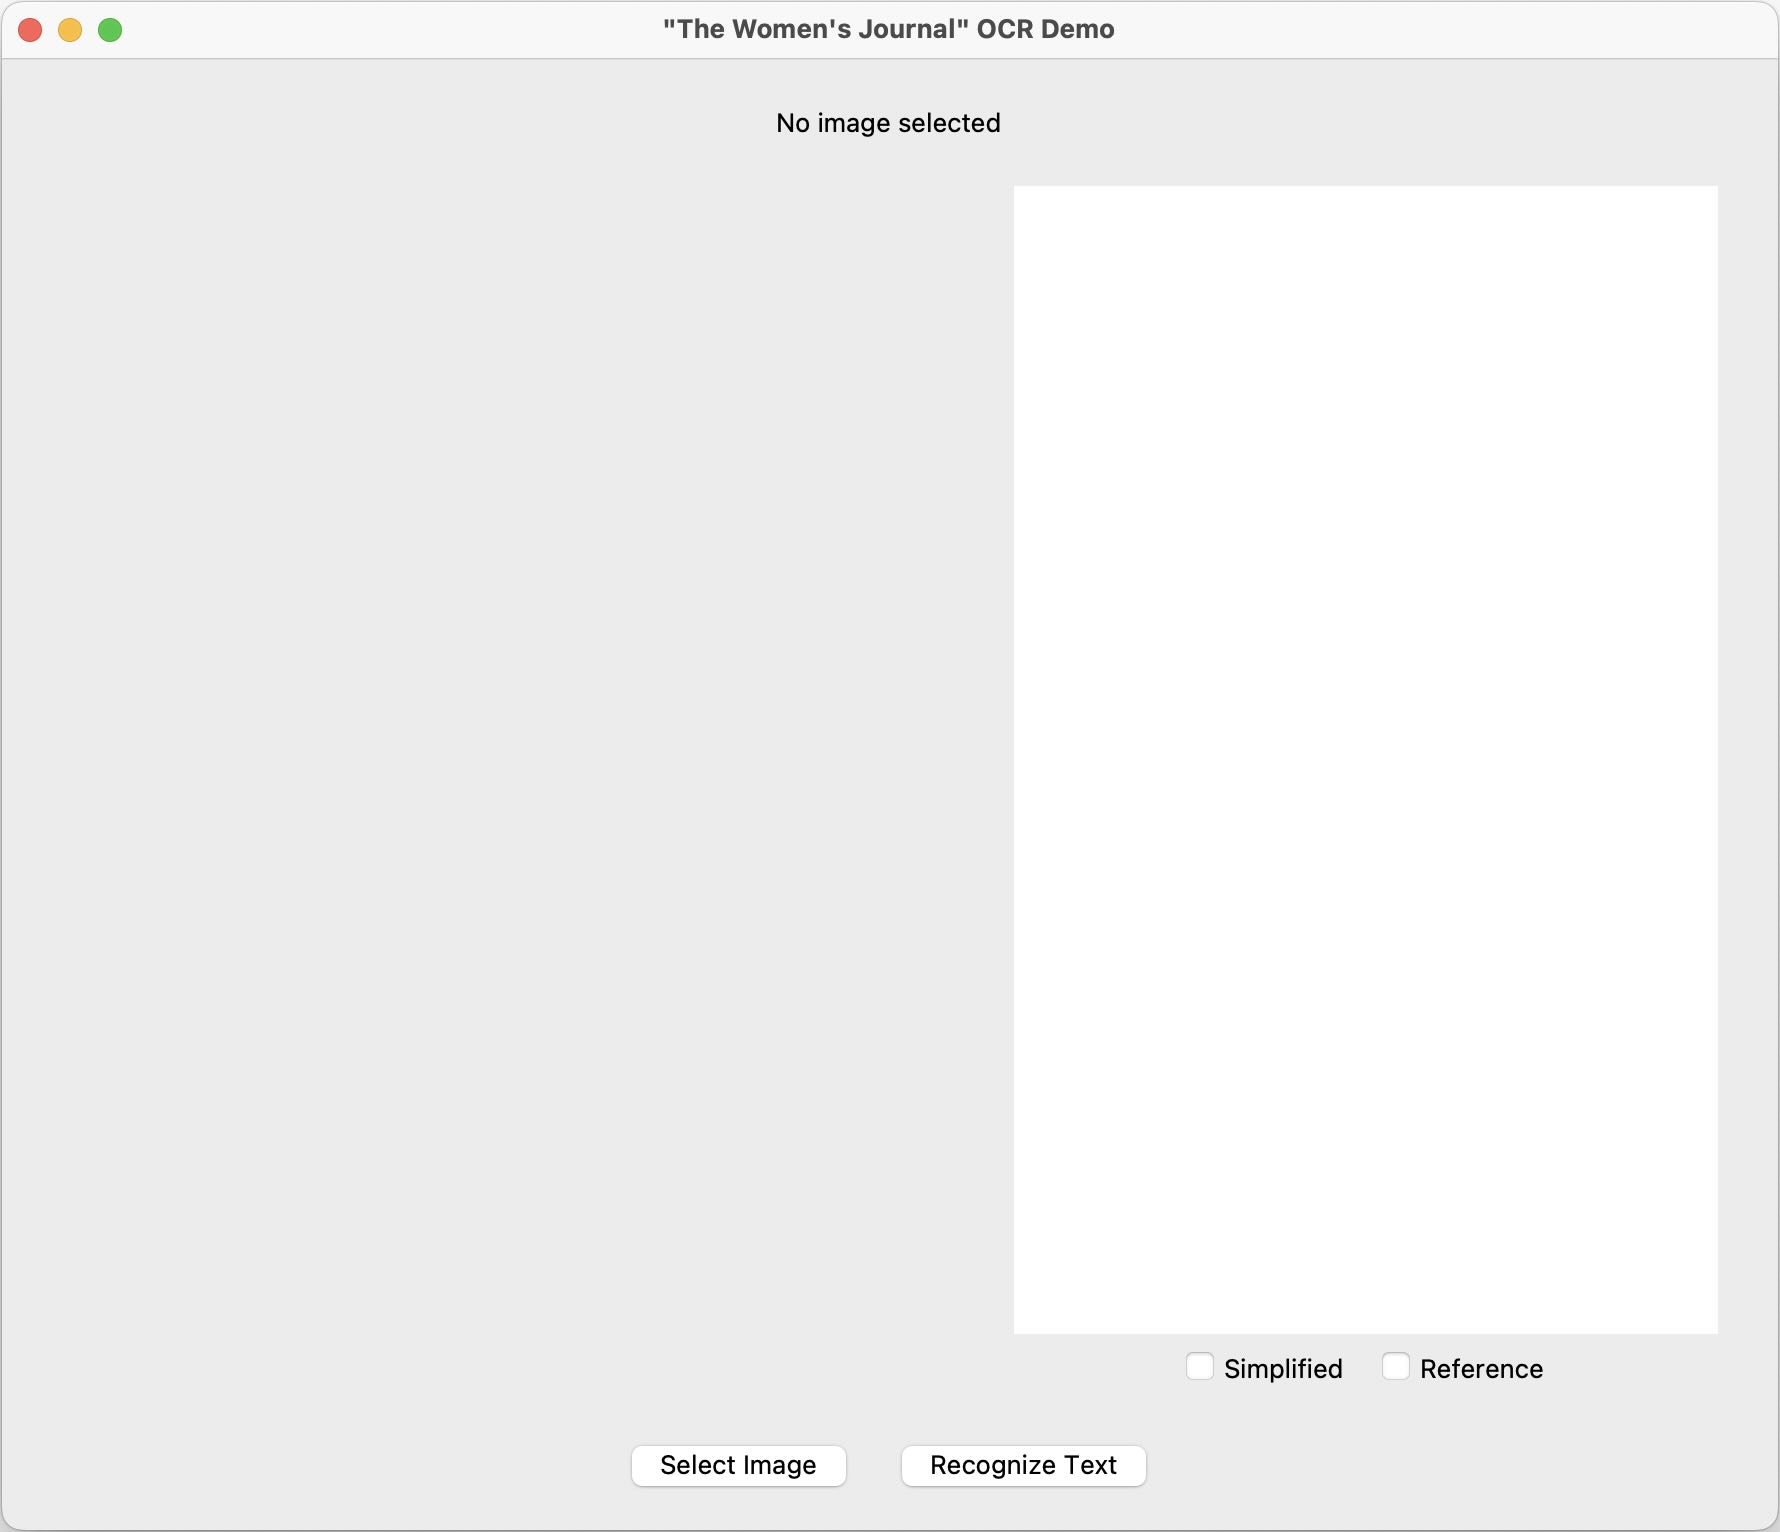
\includegraphics[width=\linewidth]{./figures/ui1.1.jpeg}
        \caption{Initial state}
        \label{fig:ui1.1}
    \end{subfigure}
    \hfill
    \begin{subfigure}[b]{0.3\linewidth}
        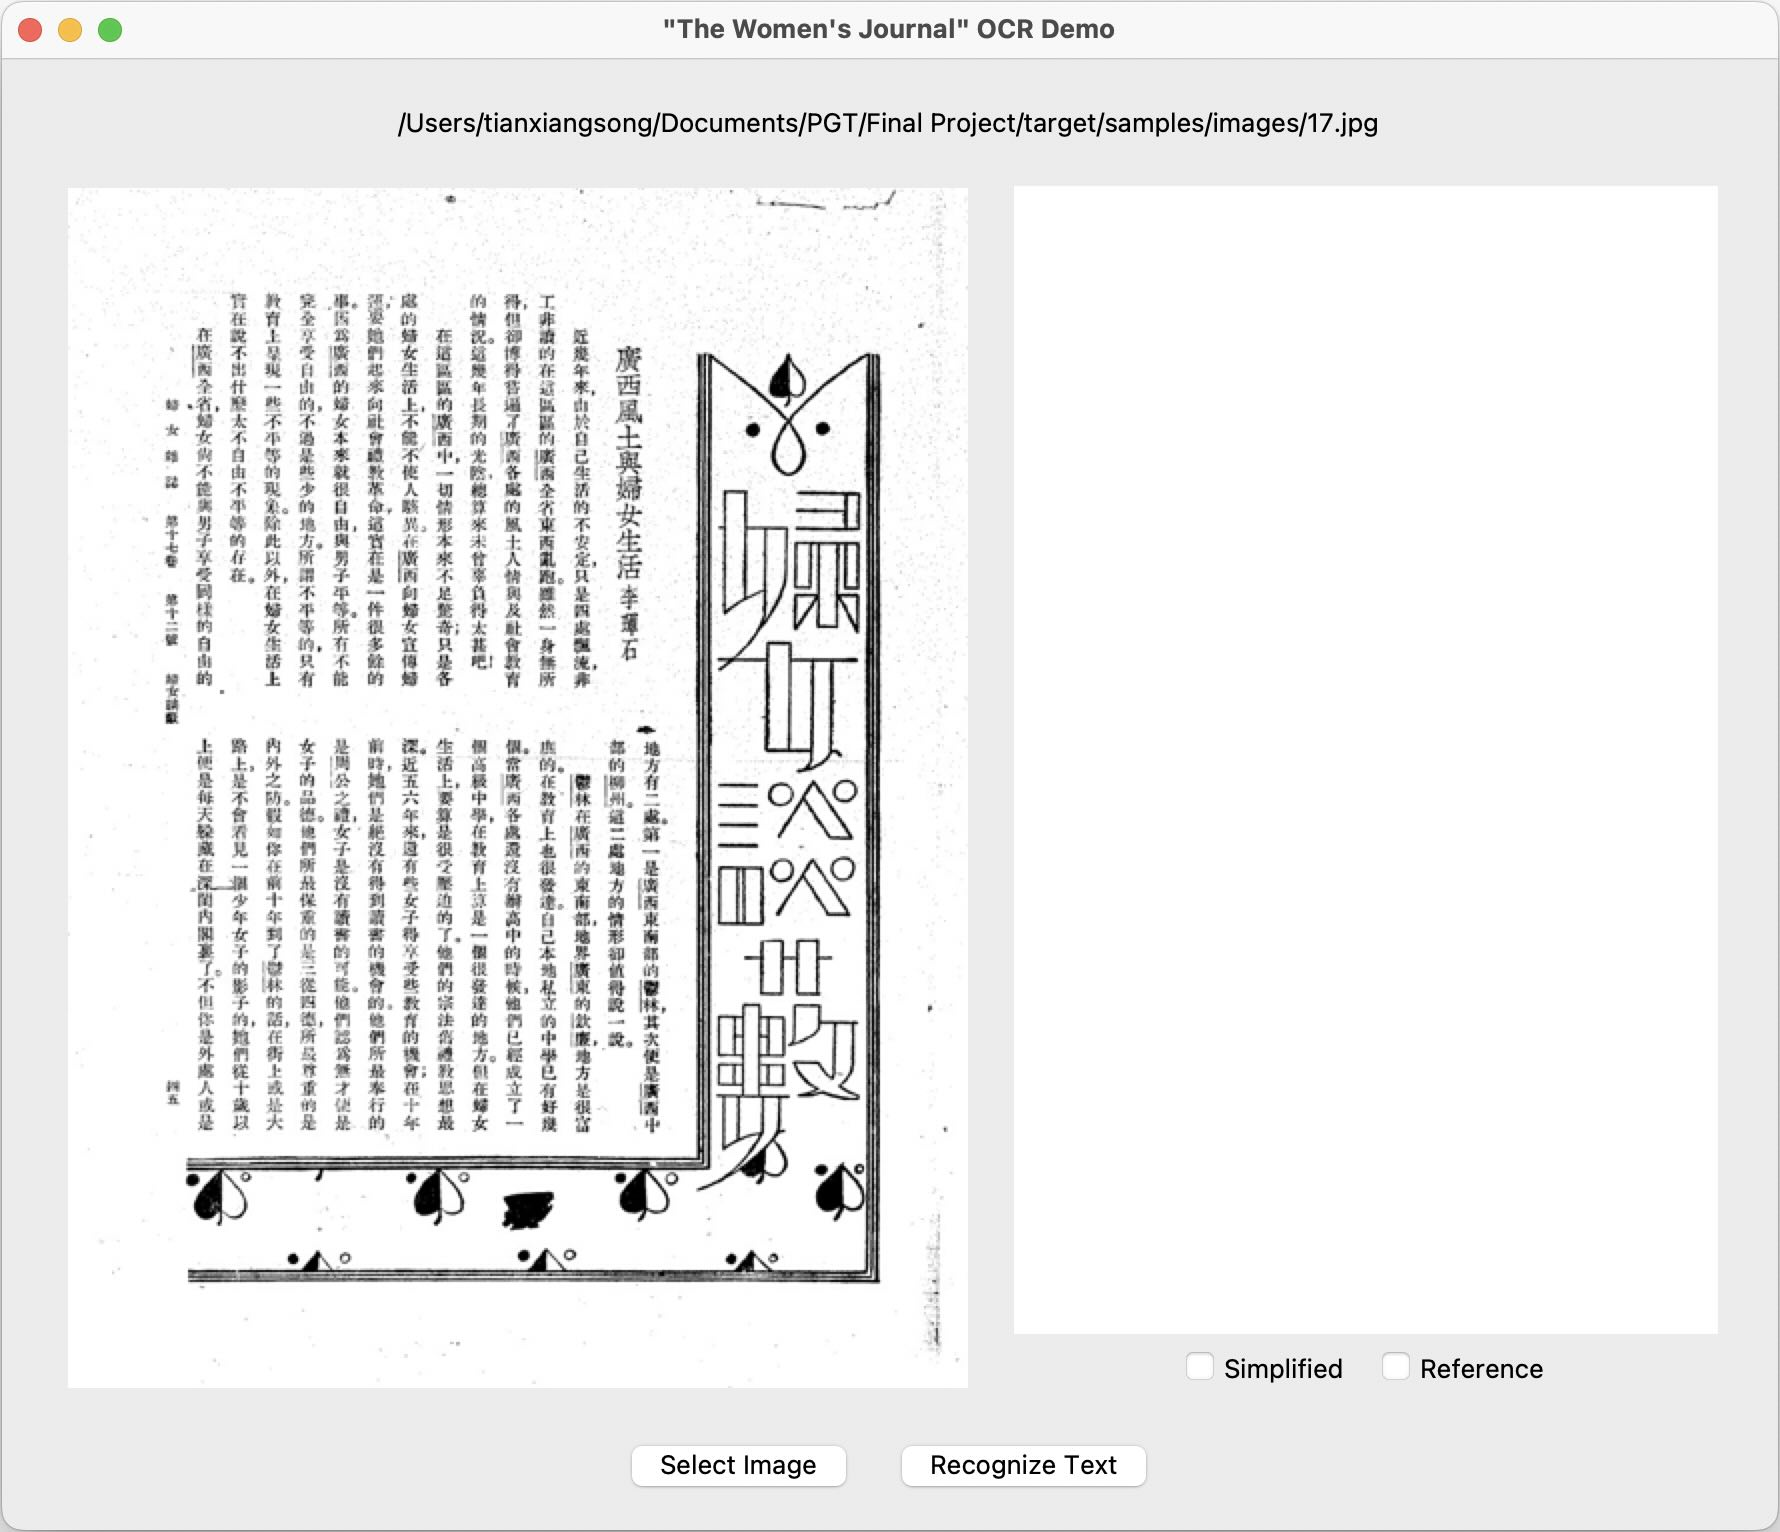
\includegraphics[width=\linewidth]{./figures/ui1.2.jpeg}
        \caption{After uploading image}
        \label{fig:ui1.2}
    \end{subfigure}
    \hfill
    \begin{subfigure}[b]{0.3\linewidth}
        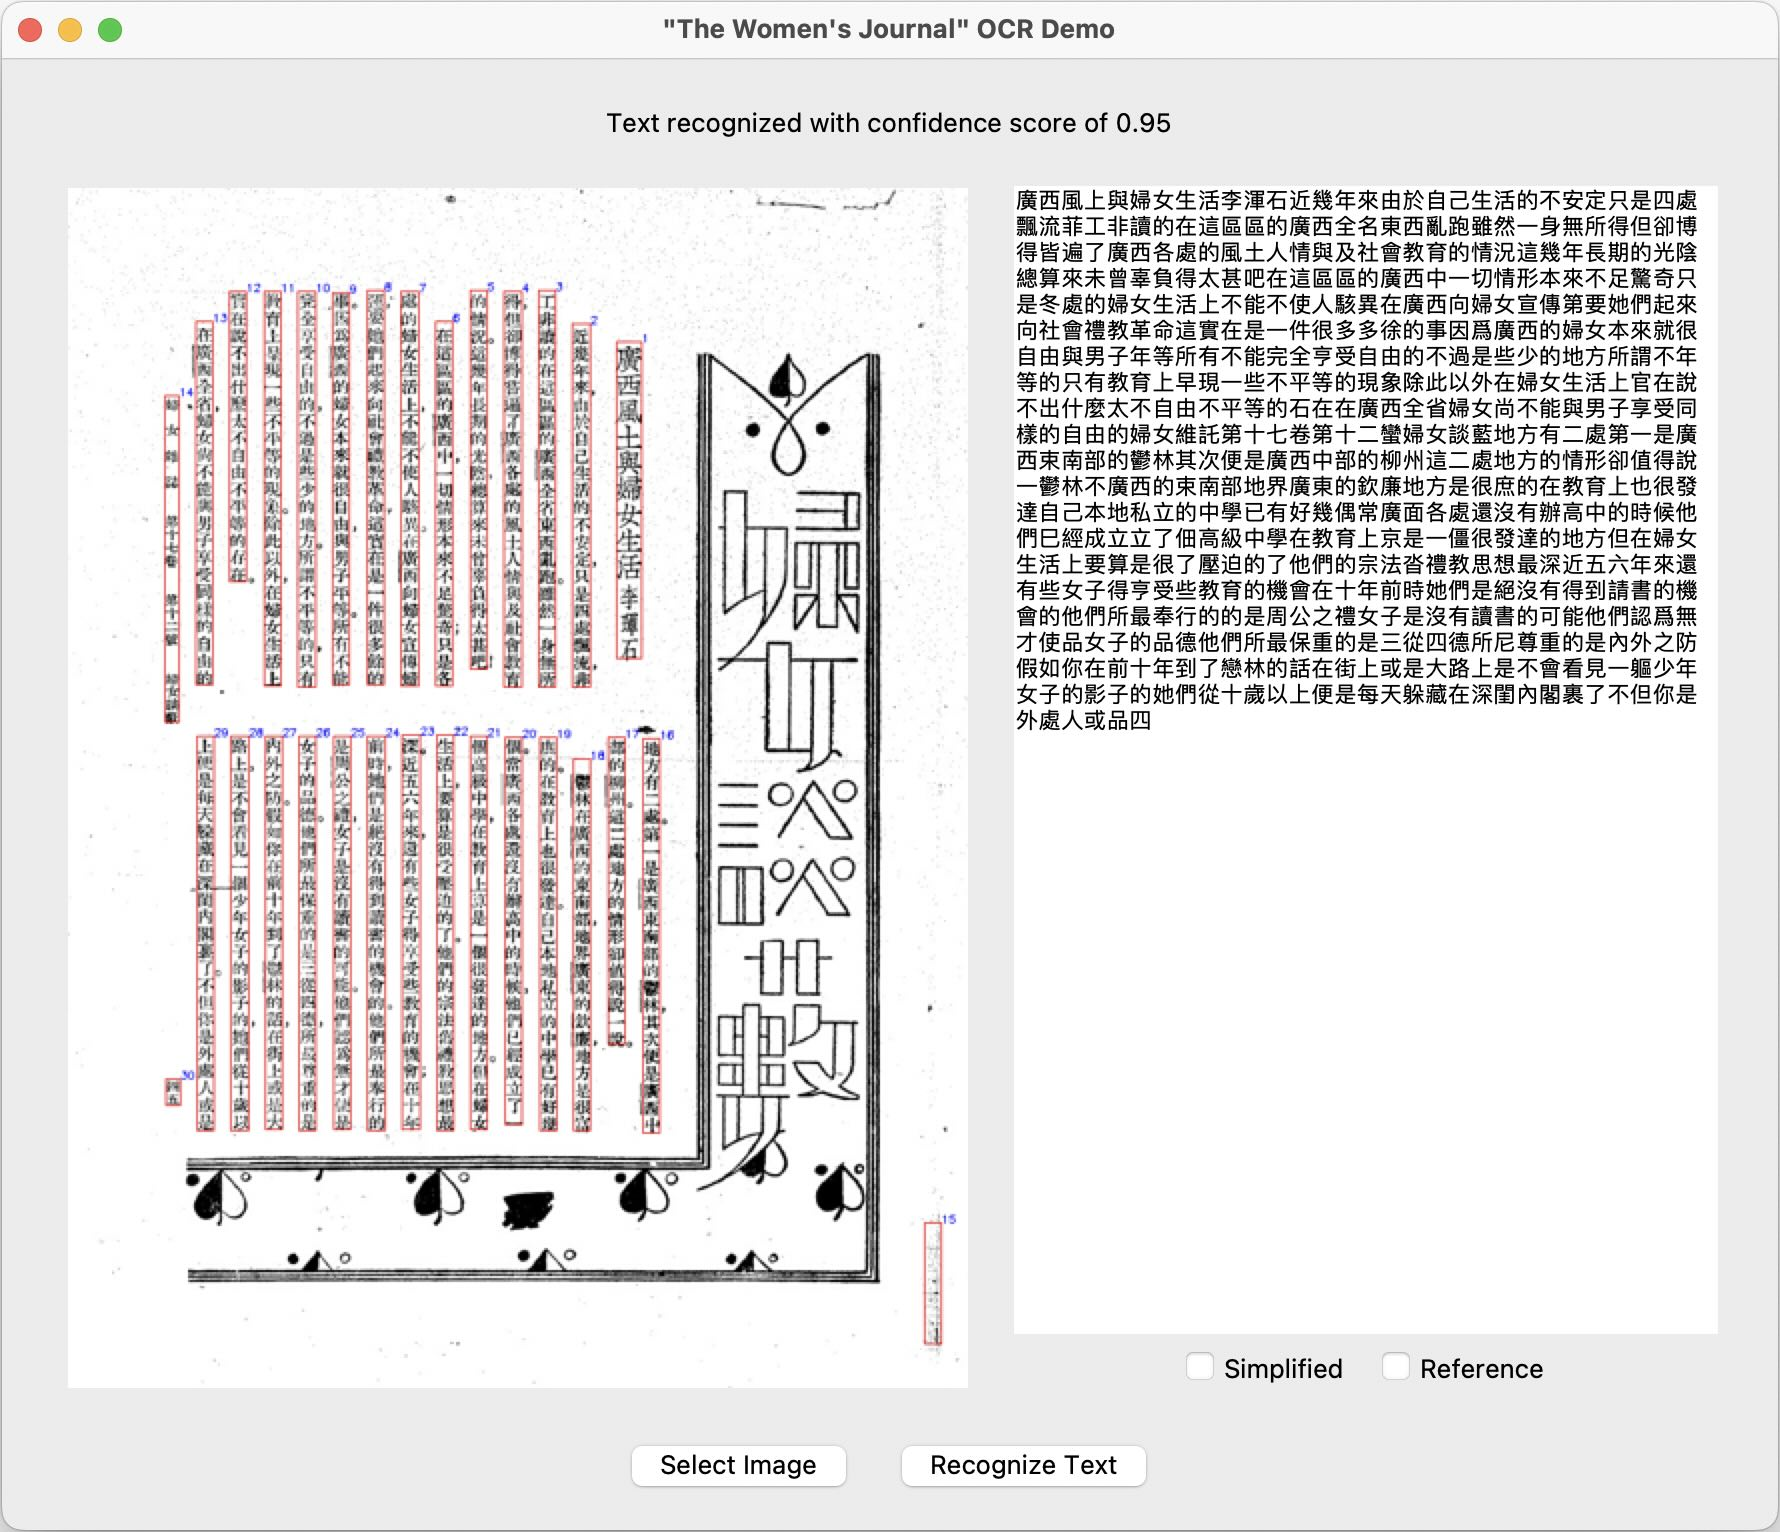
\includegraphics[width=\linewidth]{./figures/ui1.3.jpeg}
        \caption{After extracting text}
        \label{fig:ui1.3}
    \end{subfigure}

    \begin{subfigure}[b]{0.3\linewidth}
        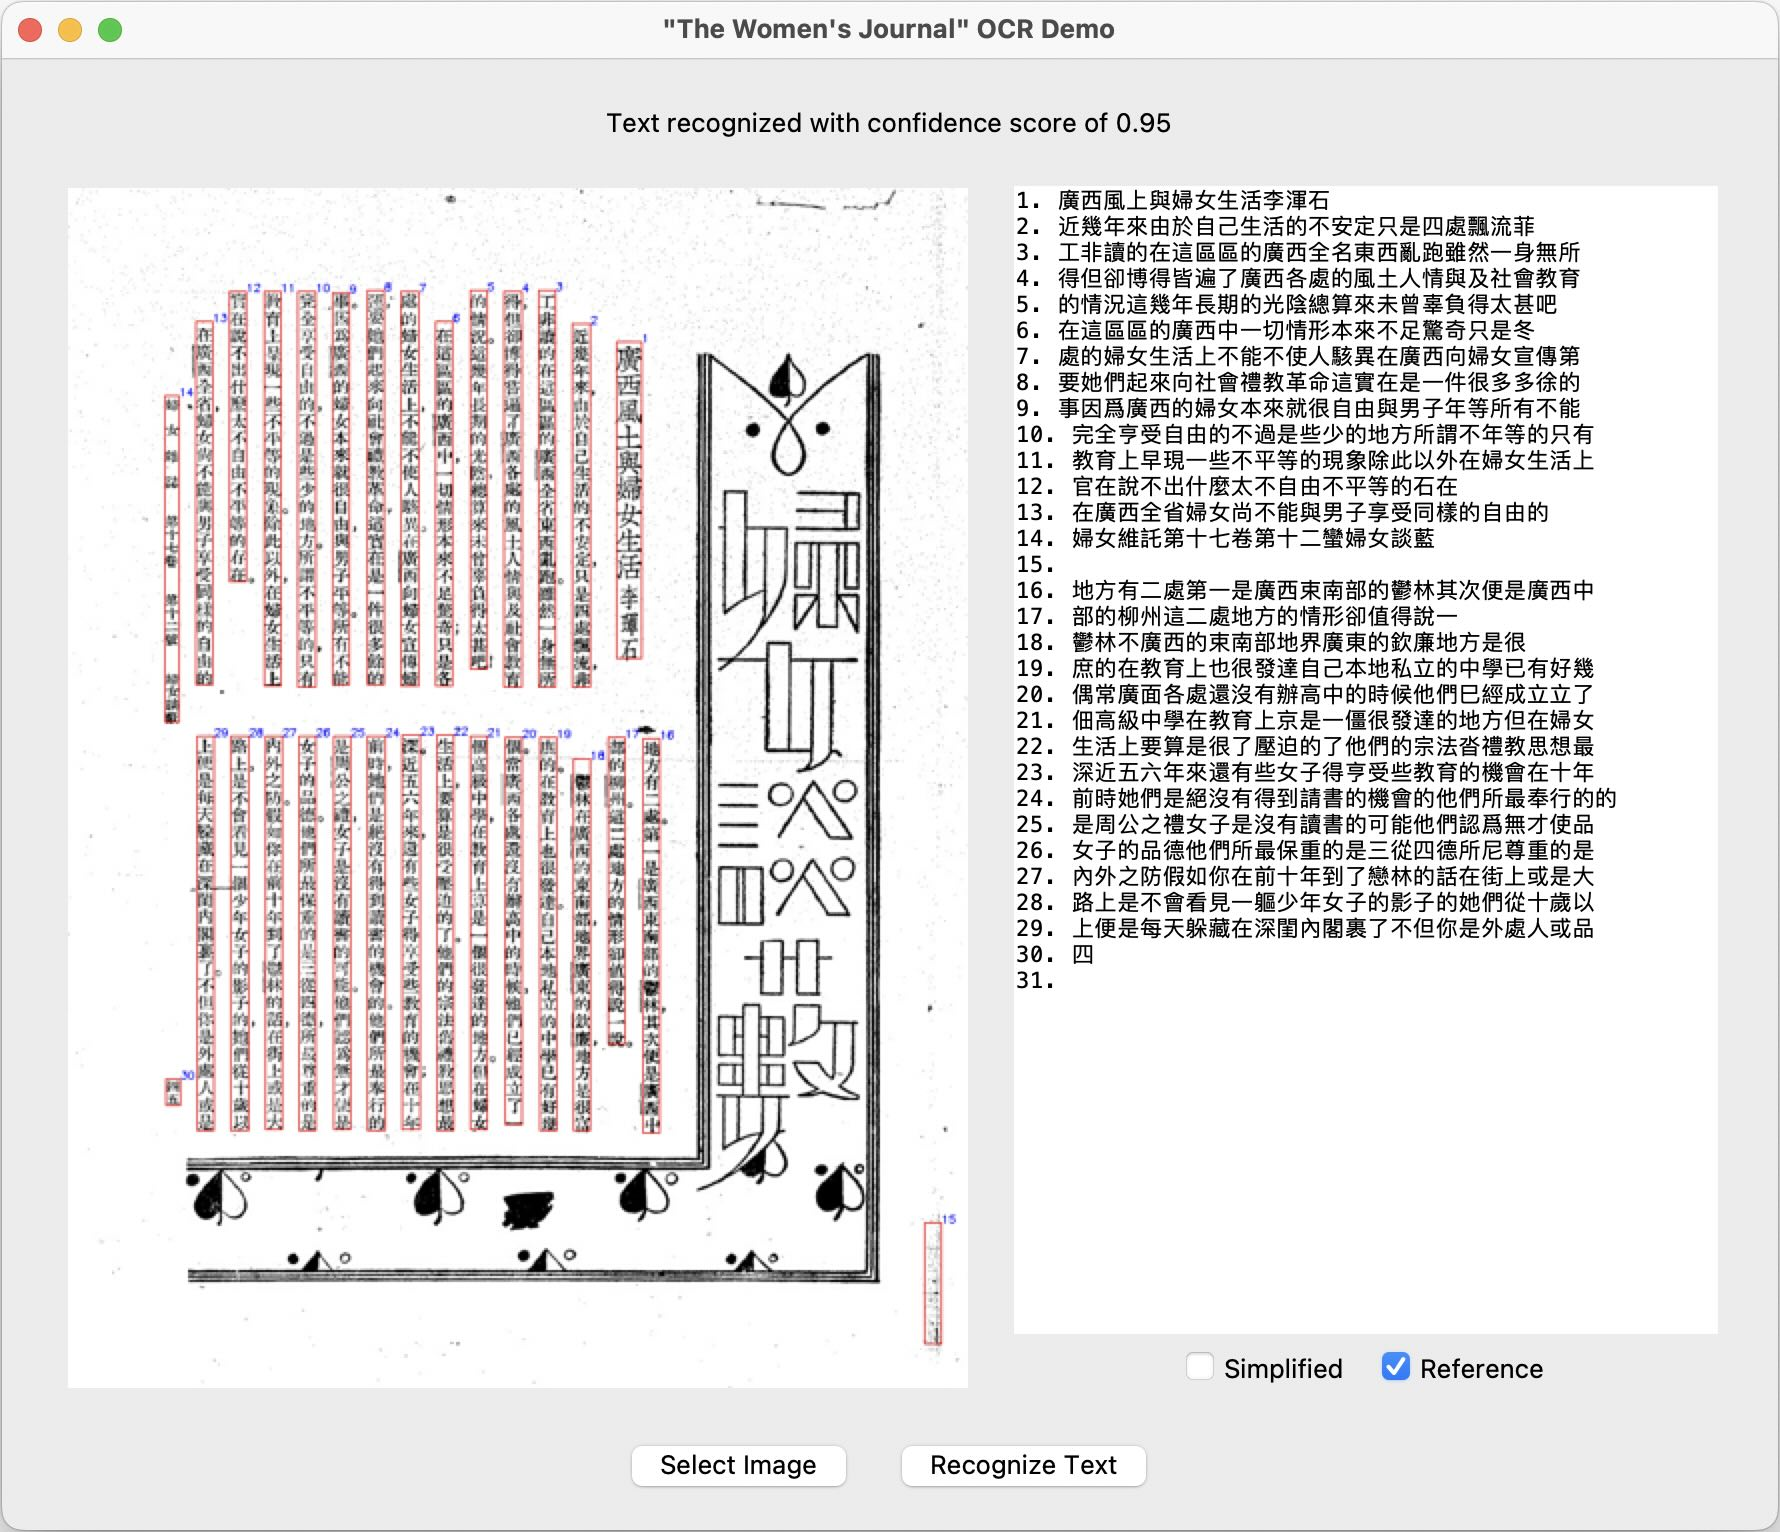
\includegraphics[width=\linewidth]{./figures/ui1.4.jpeg}
        \caption{Display textline references}
        \label{fig:ui1.4}
    \end{subfigure}
    \hfill
    \begin{subfigure}[b]{0.3\linewidth}
        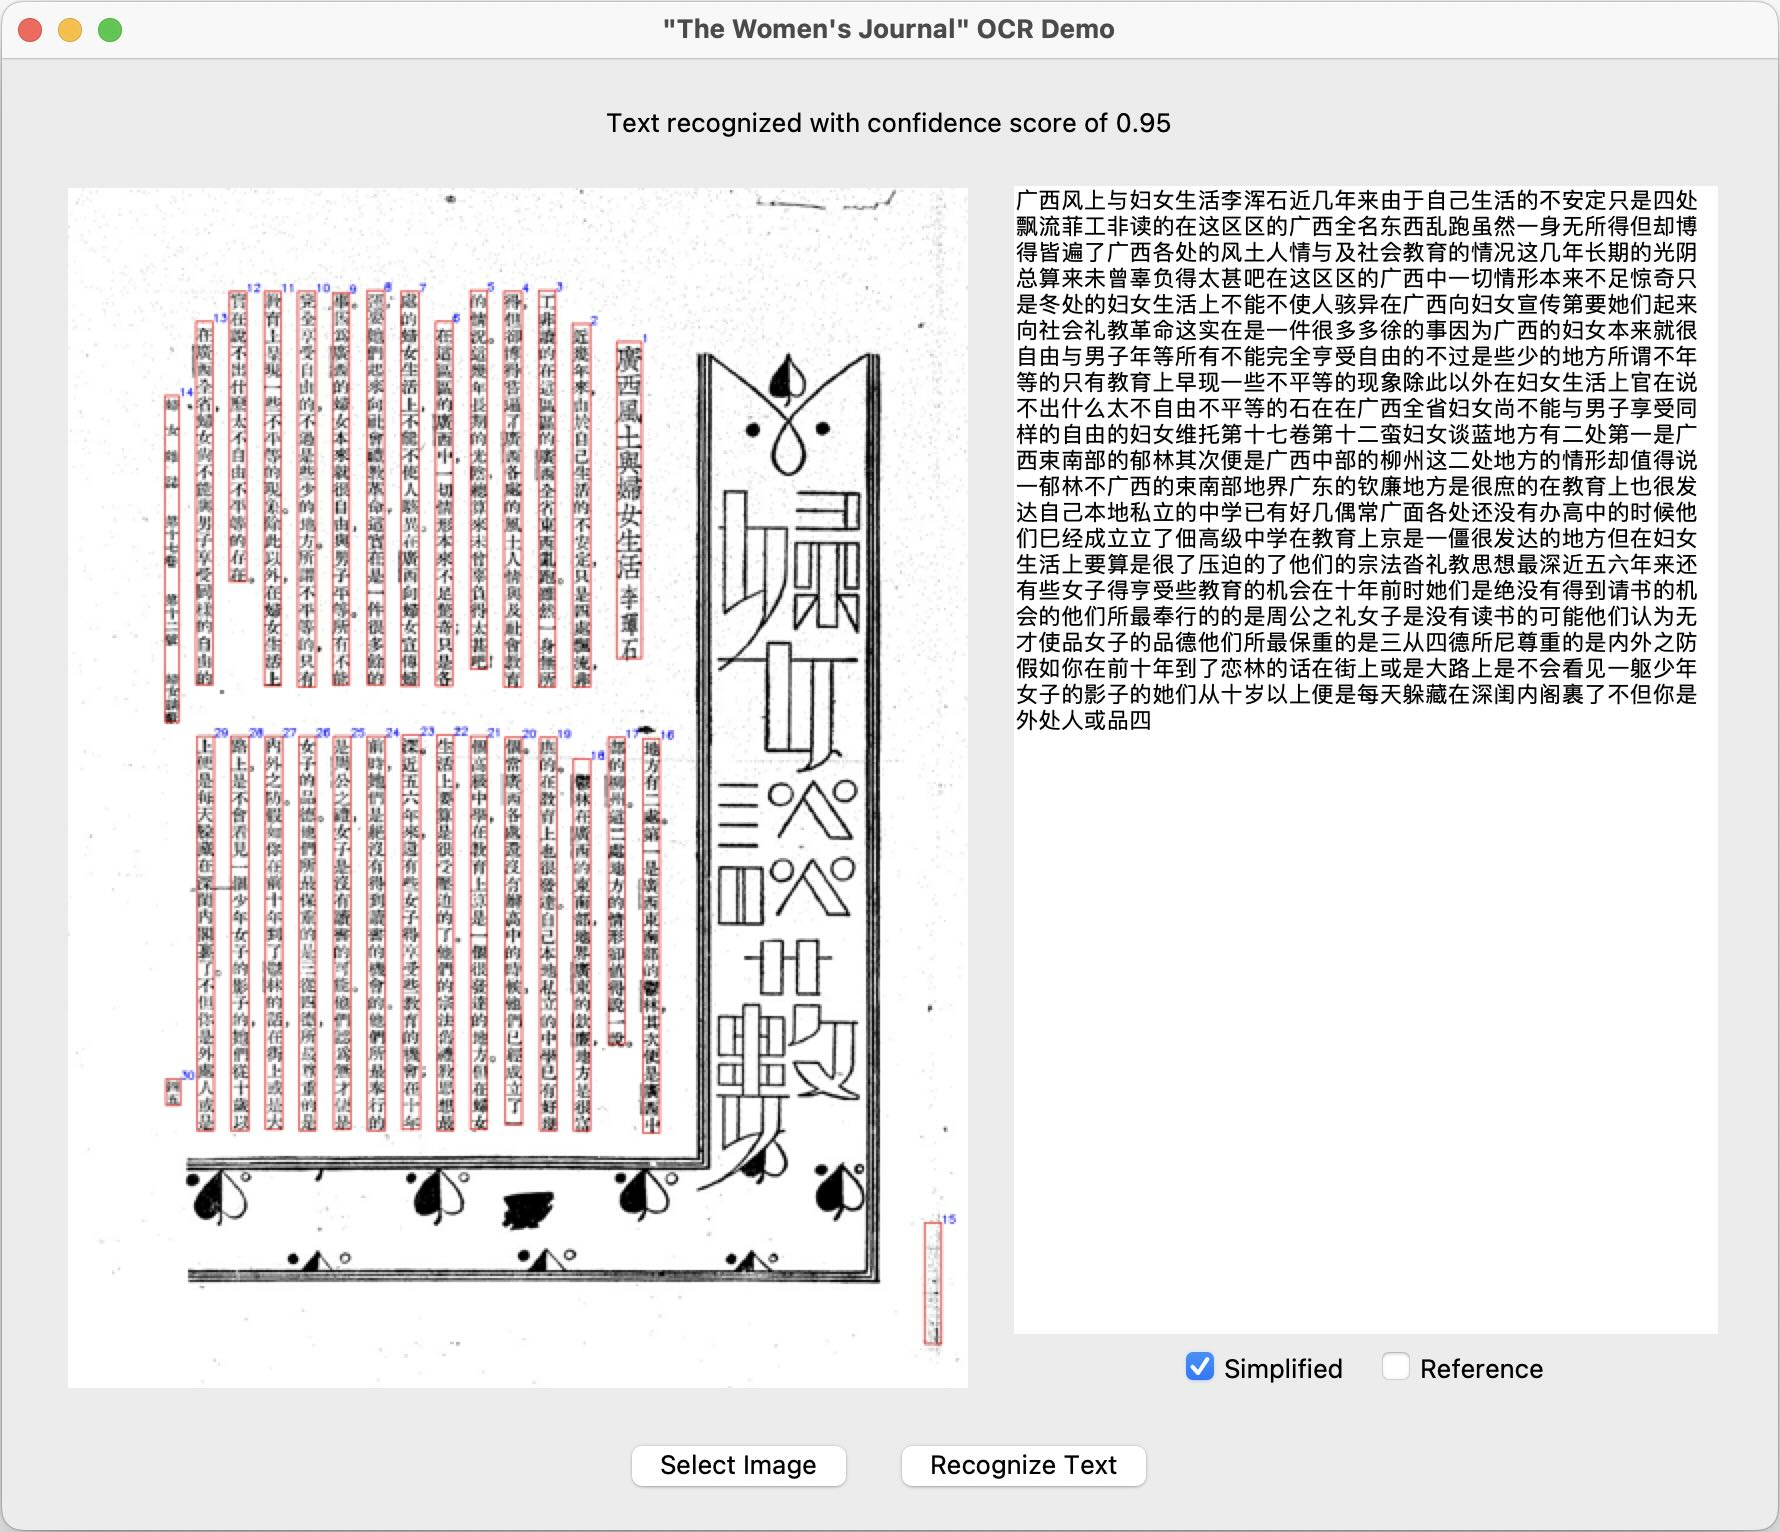
\includegraphics[width=\linewidth]{./figures/ui1.5.jpeg}
        \caption{Display simplified Chinese}
        \label{fig:ui1.5}
    \end{subfigure}
    \hfill
    \begin{subfigure}[b]{0.3\linewidth}
        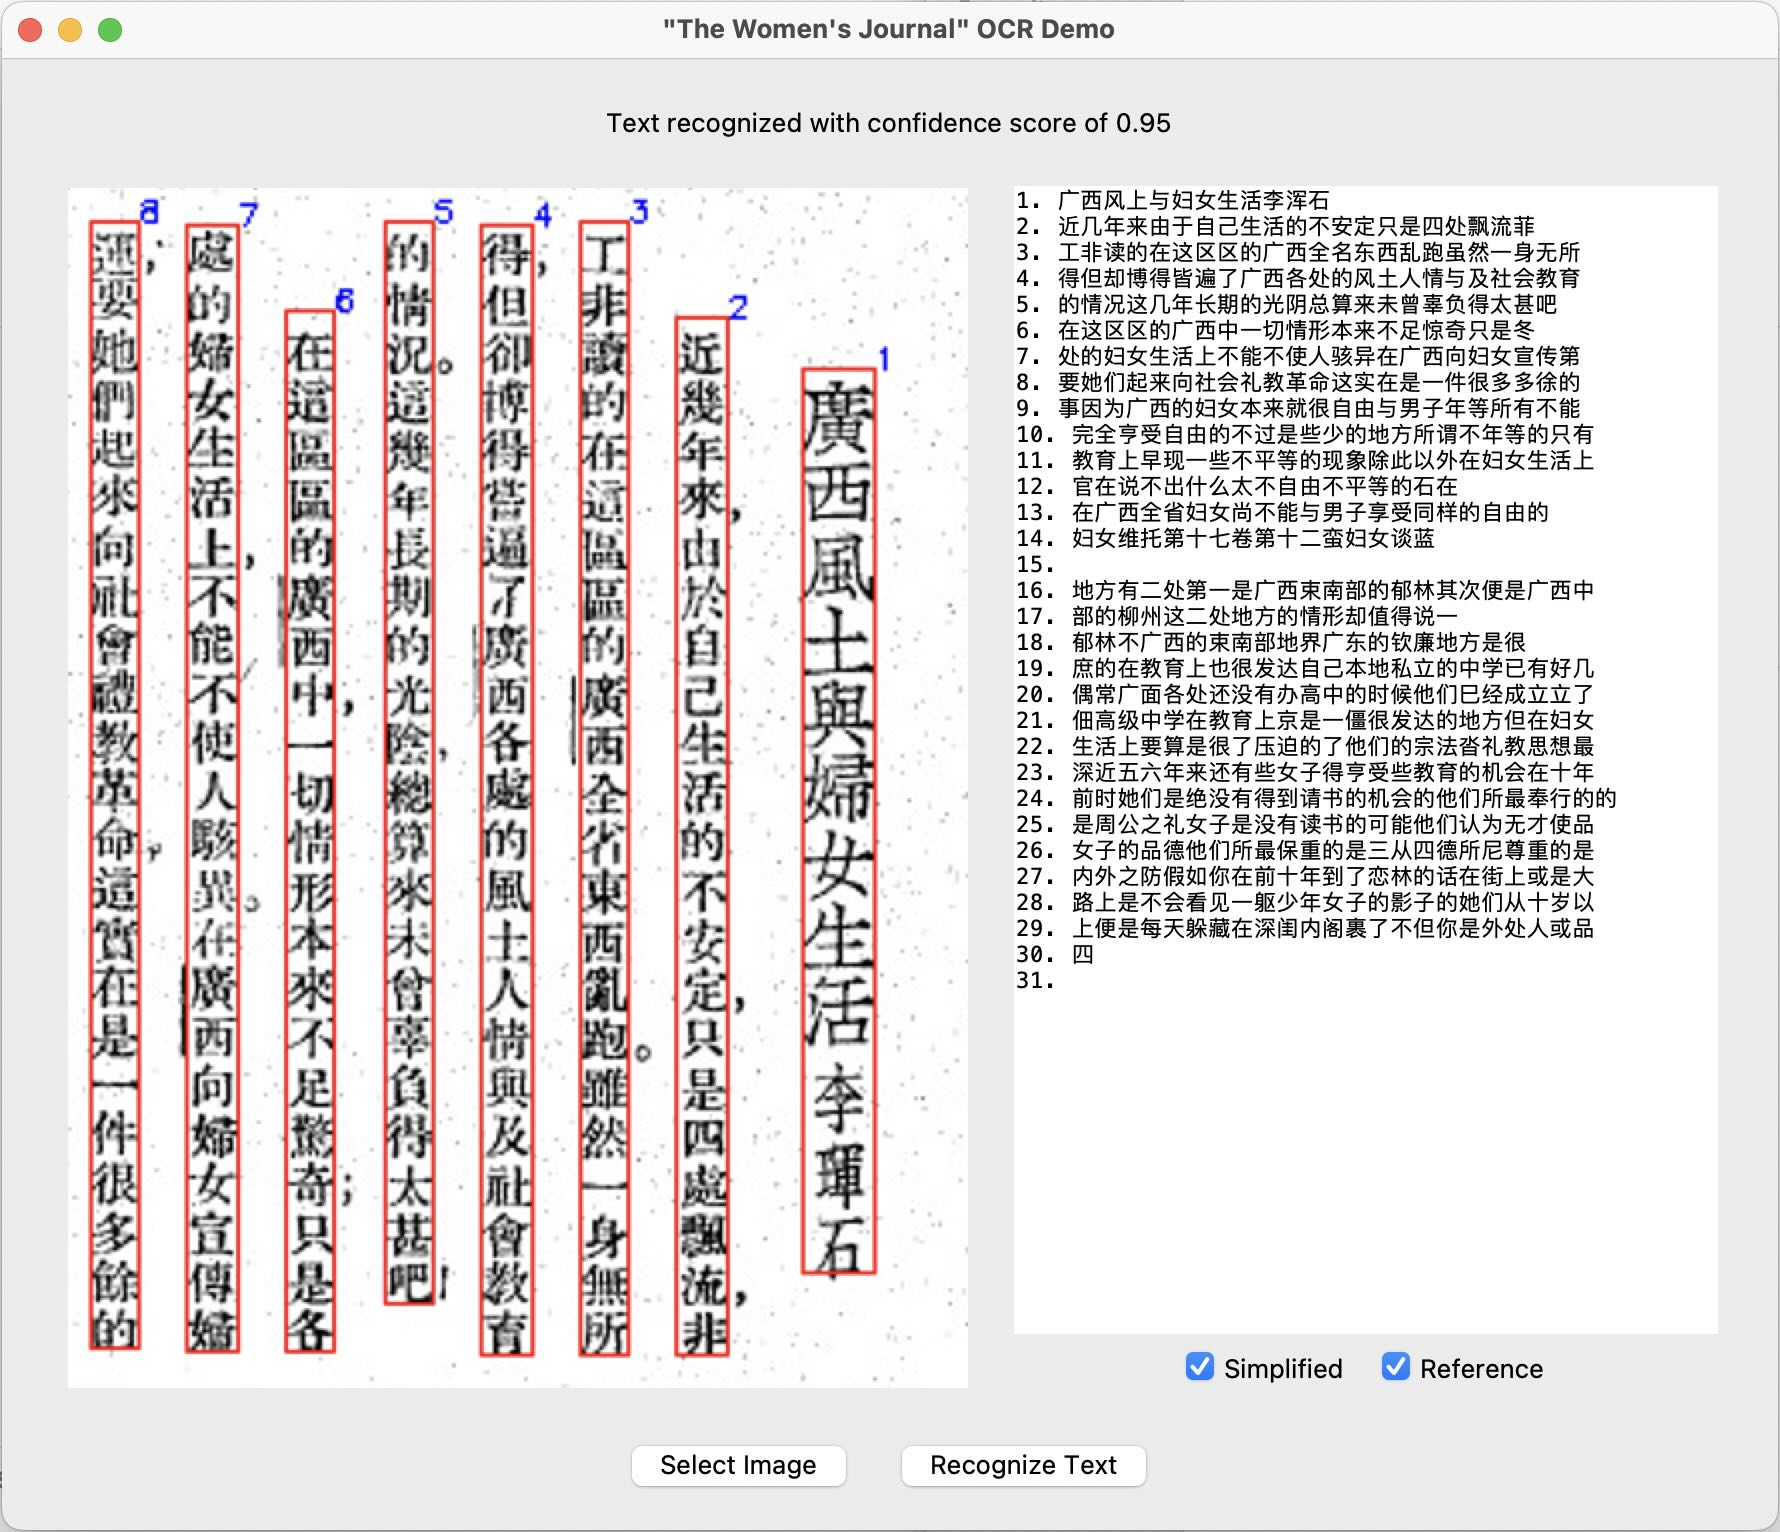
\includegraphics[width=\linewidth]{./figures/ui1.6.jpeg}
        \caption{Zoom and shift image}
        \label{fig:ui1.6}
    \end{subfigure}
    \caption{Main states and operations of the user interface}
    \label{fig:ui1}
\end{figure}

%%%%%%%%%%%%%%%%%%%%%%%%%%%%%%%%%%%%
\chapter{Evaluation}
This chapter presents the evaluation of the OCR system on the target dataset, including the experiment setup, evaluation metrics, comparison with baseline methods, and discussions on the results.

\section{Experiments}
\label{sec:experiments}
To evaluate the performance of the OCR system, we manually selected 20 images from the target dataset (Section \ref{sec:target_dataset}) as the test set, which contains a variety of text layouts and background noises to match the distribution of the whole dataset. The test set is annotated with text line positions and ordered text content for each image. The text line positions are used to evaluate the text detection model, while the recognition and ordering performance are evaluated based on the ordered text content. The images of the test set are included in Appendix \ref{app:test_images}.

We conducted a series of experiments in the optimization process, some are used for hyperparameter tuning of synthetic data generation, and some are used to optimize the inference performance. We describe these experiments in detail below.

\subsection{Text Detection Model Training}
\label{sec:text_detection_training}
The text detection model (Section \ref{sec:text_detection}) uses pre-trained weights from the COCO dataset \cite{lin2014coco}, and fine-tuned on the synthetic dataset (Section \ref{sec:synthetic_detection}) for 100 epochs using the Adam optimizer \cite{adamoptimizer} with a learning rate of $10^{-4}$, a batch size of 4, and a weight decay of $5 \times 10^{-4}$. In each epoch, we generated 1,000 images with a mix of layout L1 and L2, where we set the proportion hyperparameter $\alpha=0.8$ for layout L1 to simulate the distribution in Funü Zazhi. We conducted hyperparameter tuning on the following parameters for synthetic data generation:

\textbf{Character Size Range}: The range of font sizes used for rendering text lines in the synthetic images.

\textbf{Intensity Shift Range}: The range of intensity shift applied to the characters in the synthetic images.

\textbf{Addictive Noise Range}: The range of addictive noise intensity applied to the synthetic images. Each pixel value is added with a random noise value within the range.

\textbf{Salt and Pepper Noise Probability}: The probability of adding salt-and-pepper noise to the synthetic images. Each pixel value is set to a random value between 0 and 255 with the probability.

\textbf{Line Noise Range and Probability}: The range of line noise intensity and the probability of adding the noise to the synthetic images. The line noise is generated by drawing random-length horizontal or vertical lines on each row or column of the image with the intensity and probability.

\textbf{Erasing Probability}: The probability of erasing parts of the synthetic images. Each pixel value is set to 255 (as erased) with the probability.

\textbf{Gaussian Kernel Size and Sigma Range}: The kernel size and sigma used for Gaussian noise generation in the synthetic images.

\textbf{Max Non-text Elements}: The maximum number of non-text elements (icons) chosen from the Icons-50 dataset \cite{icons50} to be added to each synthetic image.

\textbf{Non-text Element Size Range}: The range of width and height used for resizing the non-text elements before overlaying them on the synthetic images.

During hyperparameter tuning, the model is evaluated on the test set using mean Average Precision (mAP) \cite{map}, which calculates the average precision of the text detection model at different Intersection over Union (IoU) thresholds. Specifically, we use mAP@[0.5:0.95], which is calculated as the mean of the average precision at IoU thresholds from 0.5 to 0.95 with a step size of 0.05. The best hyperparameters are selected based on the mAP score on the test set. We also performed an ablation study to evaluate the importance of each augmentation technique in the synthetic data generation process for text detection.

\subsection{Text Detection Model Inference}
\label{sec:text_detection_inference}
After the text detection model is trained using the best parameters found in Experiment \ref{sec:text_detection_training}, we conducted another experiment to optimize the inference performance. We applied a threshold to the confidence score of the detected text lines, and only kept the text lines with a confidence score higher than the threshold. The confidence score is calculated as the maximum probability of the predicted text line by the text detection model, which is used to estimate the accuracy of the detection result. We experimented with different threshold values and evaluated the model on the test set using mAP as in Experiment \ref{sec:text_detection_training}. Under the best threshold value, we plotted the precision-recall curve and calculated the average precision at different IoU thresholds. We also investigated the mAP for each test image, and analyzed the detection results to identify the common failure cases.

\subsection{Text Recognition Model Training}
\label{sec:text_recognition_training}
The text recognition model (Section \ref{sec:text_recognition}) is trained from scratch on the synthetic dataset (Section \ref{sec:synthetic_recognition}) for 500 epochs using the Adam optimizer \cite{adamoptimizer} with a learning rate of $10^{-3}$, a batch size of 32, and a scheduler that reduces the learning rate by a factor of 0.5 when the validation loss plateaus for 5 epochs. In each epoch, we generated 10,000 images with a mix of vertical and horizontal text lines, where we set the proportion hyperparameter $\beta=0.9$ for vertical lines to simulate the distribution in Funü Zazhi. In addition to the parameters used in Experiment \ref{sec:text_detection_training} (excluding those for non-text elements), we conducted hyperparameter tuning on the following parameters for synthetic data generation:

\textbf{Frequency-based Character Selection} (Bool): Whether to select characters based on their frequency in the Character Frequency List \cite{charlist}.

\textbf{Word Replacement Probability}: The probability of replacing characters with common words or phrases \cite{wordlist} in the synthetic text lines.

To evaluate the text recognition model, we use the output of the best text detection model (from Experiment \ref{sec:text_detection_inference}) to crop the detected text lines from the test images, and then feed them into the recognition model to extract the text line content, which is then ordered by text ordering Algorithm \ref{alg:ordering} with default hyperparameter value $\lambda = 0.25$. The recognition model is then evaluated on the ordered text content using the following two metrics:

\textbf{Character Error Rate (CER)}: The CER is calculated as the Levenshtein distance between the predicted text content and the ground truth text content, normalized by the total number of characters in the ground truth text content. A lower CER indicates a better recognition performance. This metric is used to evaluate the character level accuracy of the text recognition model.

\textbf{BLEU Score}: The BLEU score is calculated as the geometric mean of the n-gram precision scores between the predicted text content and the ground truth text content. Specifically, we use BLEU-4, which calculates the precision of 1-gram to 4-gram between the predicted and ground truth text content. A higher BLEU score indicates a better recognition performance. This metric captures the semantic quality of the result by evaluating the word and phrase level precision, and is robust to errors in the text ordering process.

After the experiment, the best hyperparameters are selected based on the average CER and BLEU score on the test set. Specifically, we use (BLEU-4 - CER) as the primary metric to balance the character and word level accuracy of the recognition model. We also performed an ablation study to evaluate the importance of each augmentation technique in the synthetic data generation process for text recognition.

\subsection{System Optimization}
\label{sec:system_optimization}
After the text recognition model is trained using the best parameters found in Experiment \ref{sec:text_recognition_training}, we conducted hyperparameter tuning for the whole OCR system on the following parameters to optimize the inference performance:

\textbf{Text Detection Threshold}: The threshold value used to filter out detected text lines based on their confidence score. It trades off precision and recall of the text detection model, which also affects the recognition and ordering performance as they rely on the detection result.

\textbf{Text Layout Parameter $\lambda$}: The hyperparameter used to distinguish between layout L1 and L2 in Algorithm \ref{alg:ordering}, where a higher value indicates a stricter threshold for classifying layout as L1. It affects the text ordering performance by determining which ordering algorithm to use for each image.

During hyperparameter tuning, the best set of parameters are selected based on the average CER and BLEU score on the test images as in Experiment \ref{sec:text_recognition_training}. In the end, under the optimal settings, we calculated the mAP, CER, BLEU-4 and confidence scores on each test image to analyze their underlying relationships. We aim to find a metric that can estimate the accuracy of a prediction when the ground truth is not available, which can be used to filter out low-quality prediction results.

\section{Results}
\label{sec:results}
The results of the experiments are presented in this section, including the evaluation metrics of the text detection, recognition and ordering modules.

\subsection{Mean Average Precision}
\label{sec:map}
The text detection model is evaluated on the test set using mAP@[0.5:0.95] as discussed in Section \ref{sec:experiments}. The result of ablation study in Experiment \ref{sec:text_detection_training} is shown in Table \ref{tab:map_ablation}, where we evaluate the importance of each augmentation technique by comparing the mAP score with and without the technique. When training the model without a specific technique, we keep the other hyperparameters the same as the best setting found in Experiment \ref{sec:text_detection_training}. 

\begin{table}[htbp]
    \centering
    \begin{tabular}{lcc}
        \toprule
        Technique to Remove & mAP@[0.5:0.95] (\%) & Difference (\%) \\
        \midrule
        Baseline & 69.9 & - \\
        Varying Character Size & 67.0 & \textbf{2.9} \\
        Intensity Shift & 68.4 & 1.5 \\
        Addictive Noise & 68.8 & 1.1 \\
        Salt and Pepper Noise & 68.7 & 1.2 \\
        Line-shaped Noise & 68.9 & 1.0 \\
        Erasing Parts  & 69.5 & 0.4 \\
        Gaussian Noise & 69.2 & 0.7 \\
        Non-text Elements & 68.1 & 1.8 \\
        \bottomrule
    \end{tabular}
    \caption{Ablation study of synthetic data generation for text detection}
    \label{tab:map_ablation}
\end{table}

The ablation study shows that varying character size has the most significant impact on the mAP score, followed by overlaying non-text elements. This indicates that the various font size and the presence of non-text elements in the synthetic images can better simulate the target dataset and help the text detection model generalize well. On the other hand, erasing parts of the synthetic training image has the least impact on the mAP score, the reason may be that although it simulates the occlusions in the text lines, it also introduces noise that may confuse the model.

\begin{figure}[htbp]
    \centering
    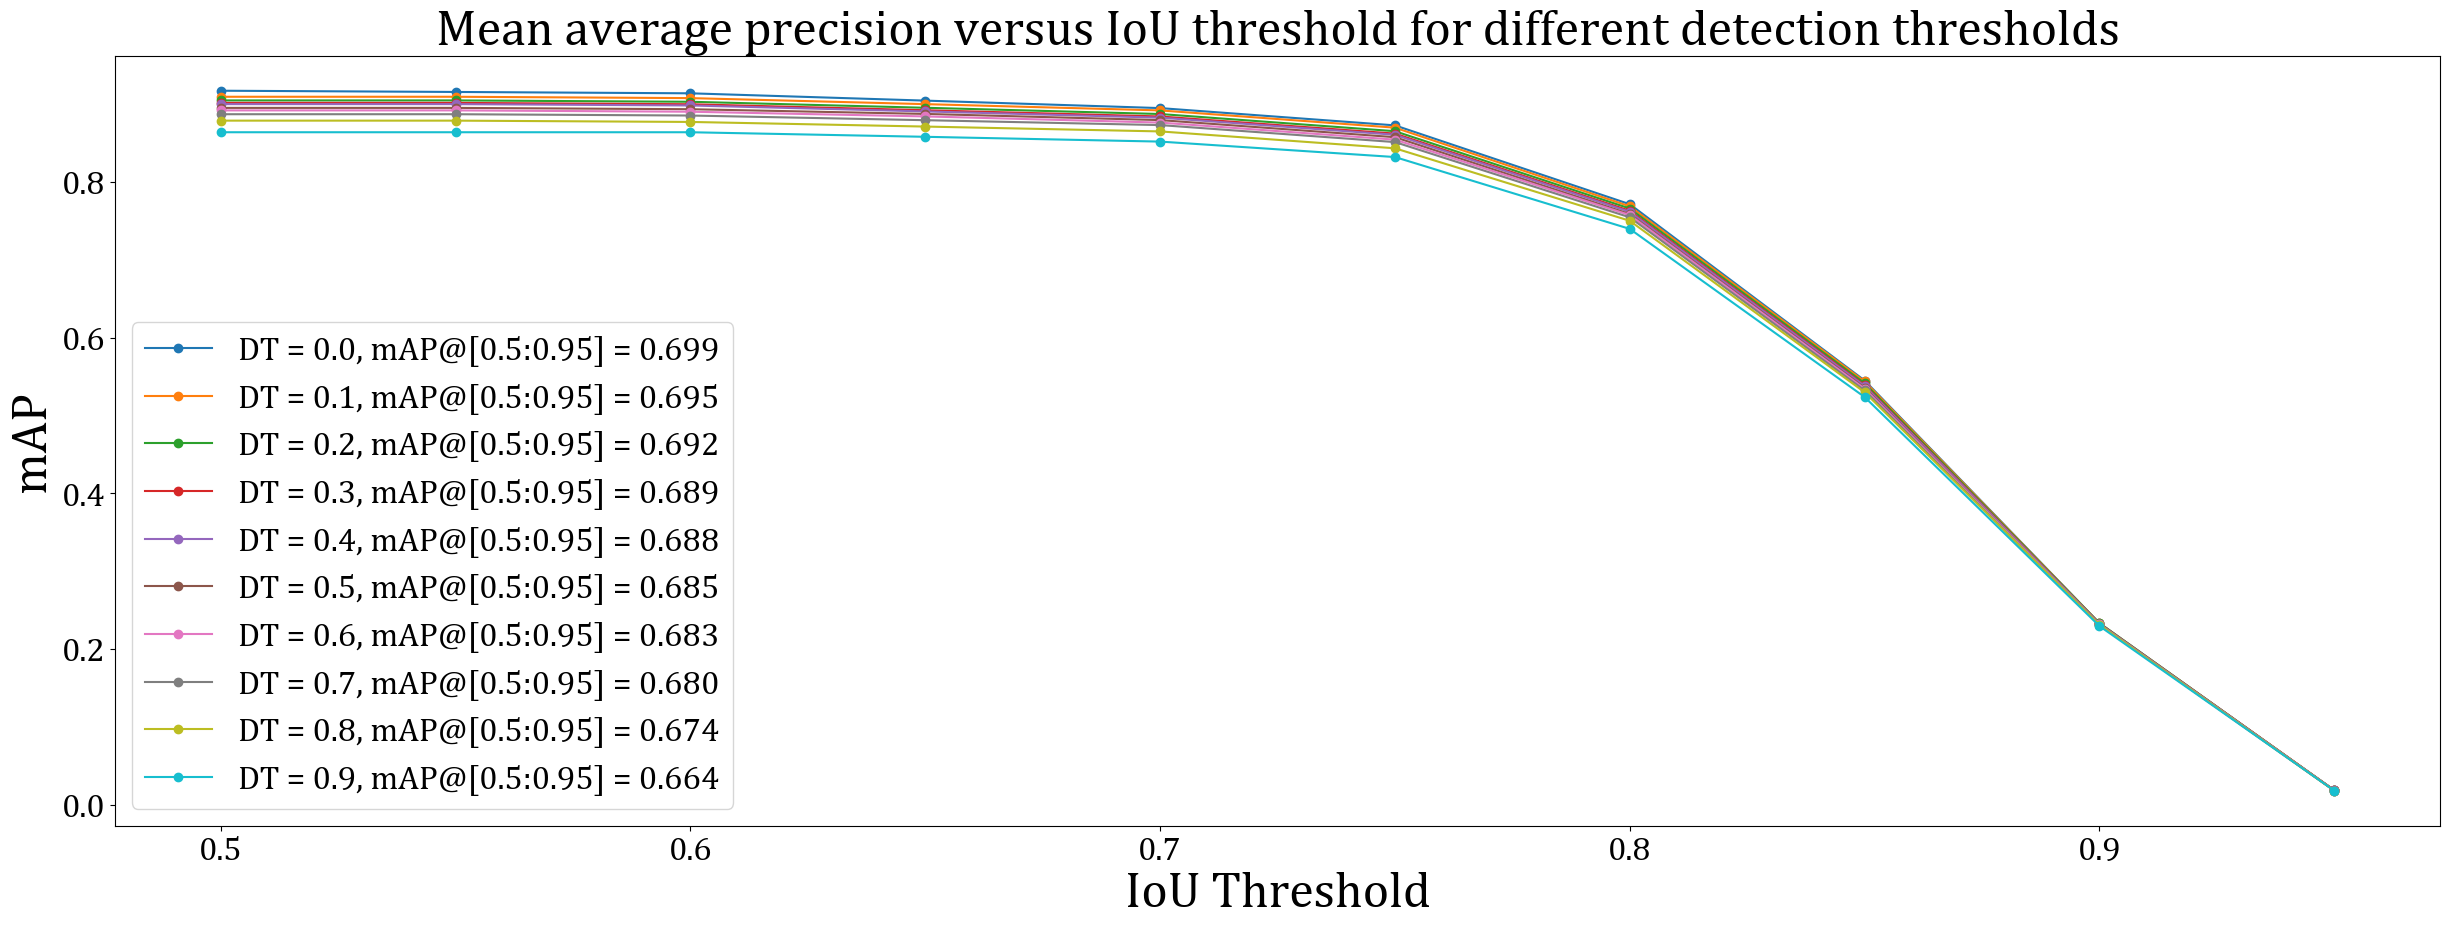
\includegraphics[width=\textwidth]{./figures/map1.png}
    \caption{Mean average precision versus loU threshold for each detection threshold}
    \label{fig:map1}
\end{figure}

The result of detection threshold optimization in Experiment \ref{sec:text_detection_inference} is shown in Figure \ref{fig:map1}, where we plot the mAP score at different IoU thresholds for each detection threshold. The result shows that the detection threshold of 0 gives the highest mAP, and the mAP decreases as the detection threshold increases, which means that the model performs best when it detects all text lines regardless of the confidence score. This indicates that the threshold may filter out some true positive detections, and the model may still make correct predictions even with low detection confidence.

\begin{figure}[htbp]
    \centering
    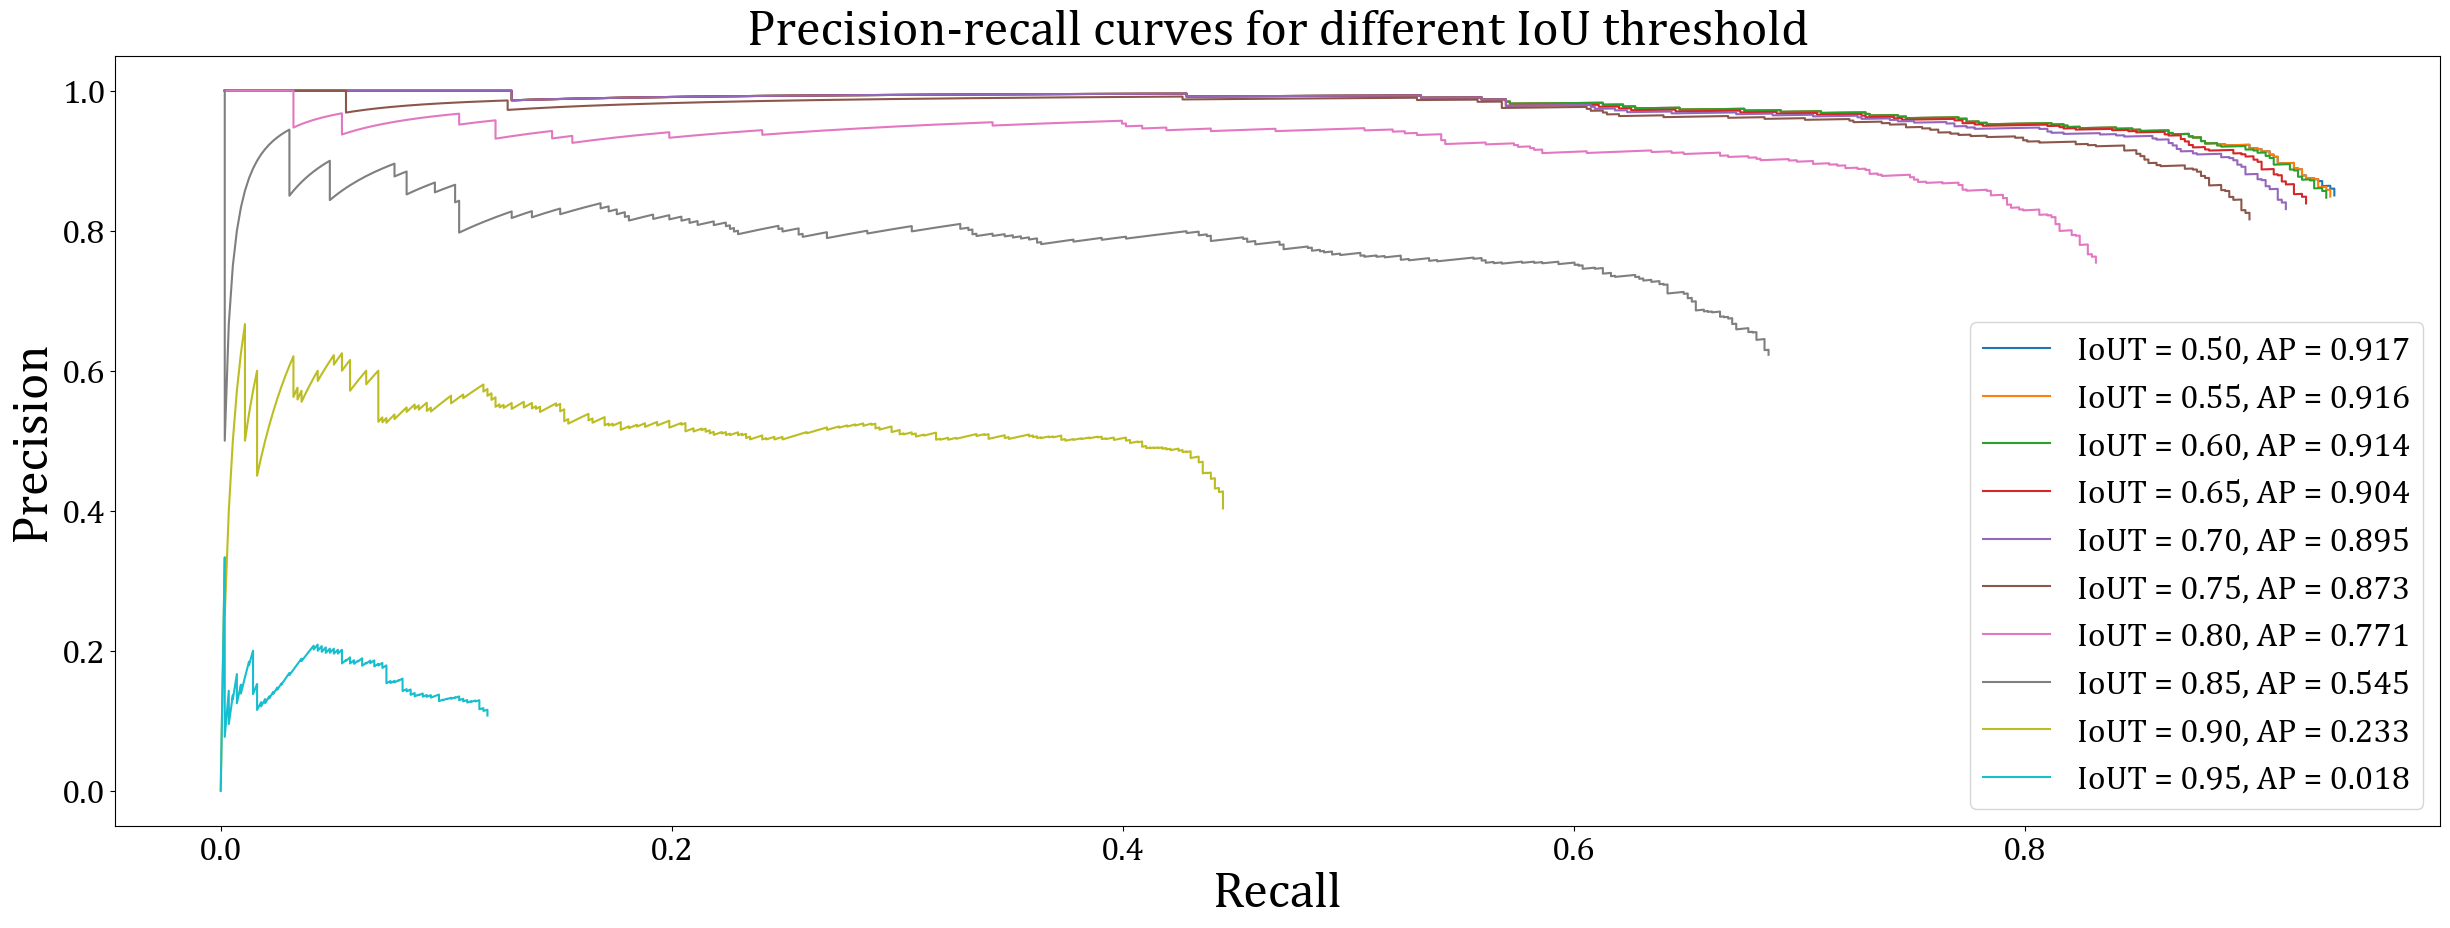
\includegraphics[width=\textwidth]{./figures/map2.png}
    \caption{Precision-recall curves of vertical text lines for each loU threshold}
    \label{fig:map2}
\end{figure}

Under the best detection threshold which achieves the mAP@[0.5:0.95] of 69.9\%, we plot the precision-recall curve and calculate the average precision (AP, or the area under the curve) of vertical lines (the majority text line type in Funü Zazhi) at different IoU thresholds, as shown in Figure \ref{fig:map2}. The result shows that the model performs well with AP above 0.75 for IoU thresholds from 0.5 to 0.8, indicating that the model can accurately detect the vertical text lines in the test set, which is crucial for the text recognition process.

\begin{figure}[htbp]
    \centering
    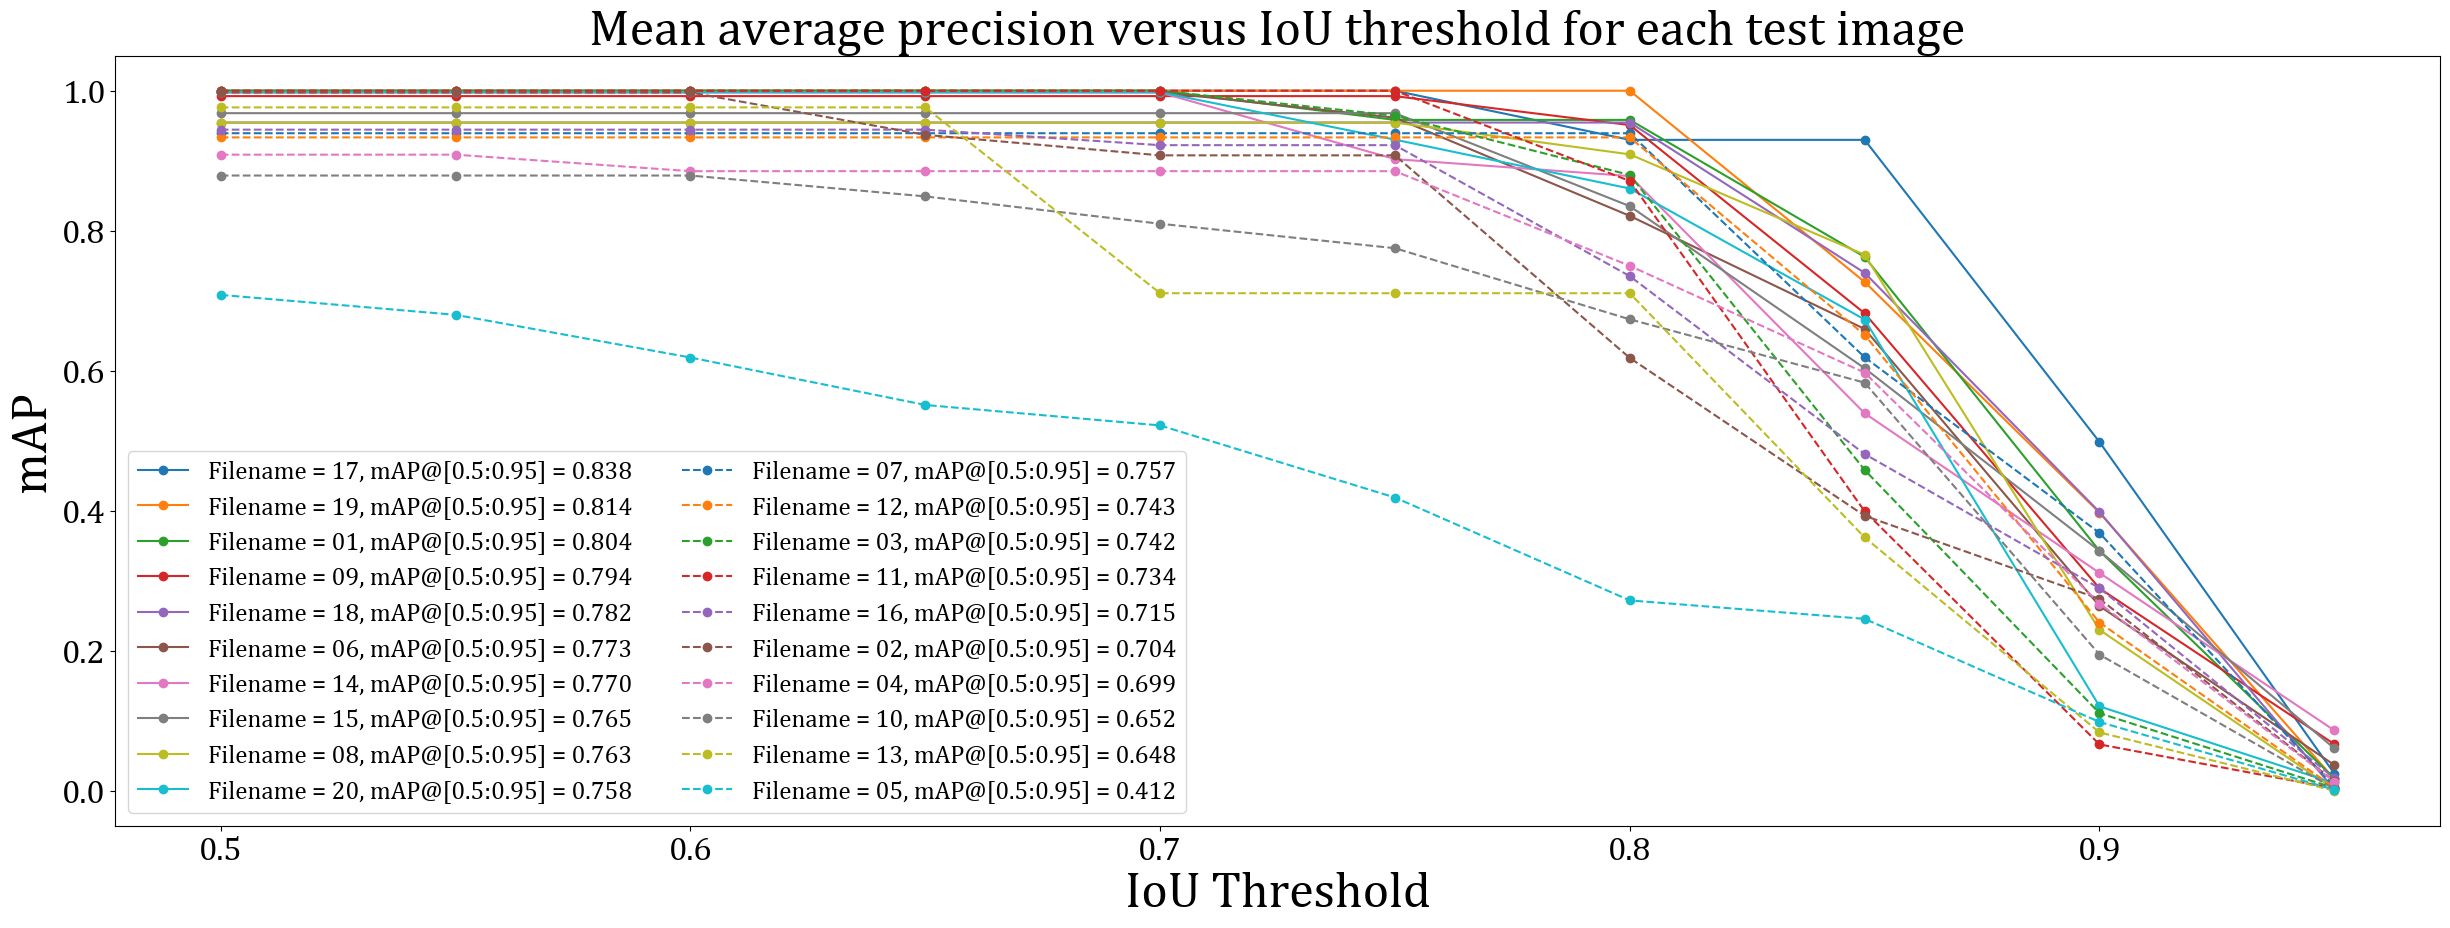
\includegraphics[width=\textwidth]{./figures/map3.png}
    \caption{Mean average precision versus loU threshold for each test image}
    \label{fig:map3}
\end{figure}

We also investigate the mAP for each test image at the optimal settings, as shown in Figure \ref{fig:map3}. It is observed that the model performs well on most images with mAP above 0.7, while there is only one image with mAP below 0.5. This indicates that the model can generalize well to most text layouts in Funü Zazhi, but may still struggle with some specific layouts that are not well covered in the synthetic dataset. We will present some detection results and analyze common failure cases in Section \ref{sec:discussions}.

\subsection{CER and BLEU Score}
\label{sec:cer_bleu}
The text recognition model is evaluated on the test set using the CER and BLEU score as discussed in Section \ref{sec:experiments}. The result of ablation study in Experiment \ref{sec:text_recognition_training} is shown in Table \ref{tab:cer_bleu_ablation}, where we evaluate the importance of each augmentation technique by comparing the CER and BLEU score with and without the technique. When training the model without a specific technique, we keep the other hyperparameters the same as the best setting found in Experiment \ref{sec:text_recognition_training}.

\begin{table}[htbp]
    \centering
    \begin{tabular}{lccc}
        \toprule
        Technique to Remove & CER & BLEU-4 & Difference (\%) \\
        \midrule
        Baseline & 0.328 & 0.546 & - \\
        Frequency-based Character Selection & 0.401 & 0.479 & \textbf{7.3} / 6.7 \\
        Word Replacement & 0.389 & 0.462 & 6.1 / \textbf{8.4} \\
        Varying Character Size & 0.352 & 0.517 & 2.4 / 2.9 \\
        Intensity Shift & 0.345 & 0.528 & 1.7 / 1.8 \\
        Addictive Noise & 0.334 & 0.539 & 0.6 / 0.7 \\
        Salt and Pepper Noise & 0.339 & 0.534 & 1.1 / 1.2 \\
        Line-shaped Noise & 0.342 & 0.531 & 1.4 / 1.5 \\
        Erasing Parts & 0.331 & 0.541 & 0.3 / 0.5 \\
        Gaussian Noise & 0.332 & 0.540 & 0.4 / 0.6 \\
        \bottomrule
    \end{tabular}
    \caption{Ablation study of synthetic data generation for text recognition}
    \label{tab:cer_bleu_ablation}
\end{table}

The ablation study shows that frequency-based character selection and word replacement have the most significant impact on the CER and BLEU score. Specifically, eabling frequency-based character selection decreases the CER by 7.3\%, while enabling word replacement increases the BLEU-4 score by 8.4\%, both of which are the highest among all techniques. This indicates that selecting characters based on their frequency can significantly improve the character level accuracy, while replacing characters with common words can improve the word and phrase level precision to a large extent. Comparing to other techniques, they can better simulate the distribution of characters and words in the target dataset, and help the text recognition model generalize well. On the other hand, erasing parts of the synthetic training image has the least impact on the CER and BLEU score, which is consistent with the result in the text detection ablation study (Table \ref{tab:map_ablation}) for similar reasons.

The result of hyperparameter tuning for system optimization in Experiment \ref{sec:system_optimization} is shown in Figure \ref{fig:cer_bleu}, where we plot the CER and BLEU-4 score versus the layout parameter $\lambda$ in Algorithm \ref{alg:ordering} (where a higher $\lambda$ indicates a stricter threshold for classifying layout as L1). The CER and BLEU-4 for all detection thresholds are plotted as red and blue lines respectively, while (BLEU-4 - CER) for each detection threshold is plotted with different colors as the primary metric. The result shows that under all detection thresholds, the CER is stable with $\lambda<0.3$, increases slightly with $0.3<\lambda<0.4$, and increases significantly with $\lambda>0.4$. On the other hand, the BLEU-4 score is stable across all values of $\lambda$, only drops slightly with $\lambda>0.4$. This suggests that the BLEU-4 score is robust to errors in the text ordering process, while the CER is sensitive to the text order. We also noticed that the maximum (BLEU-4 - CER) value is usually achieved at $\lambda=0.25$, the medium value in the tuning range.

\begin{figure}[htbp]
    \centering
    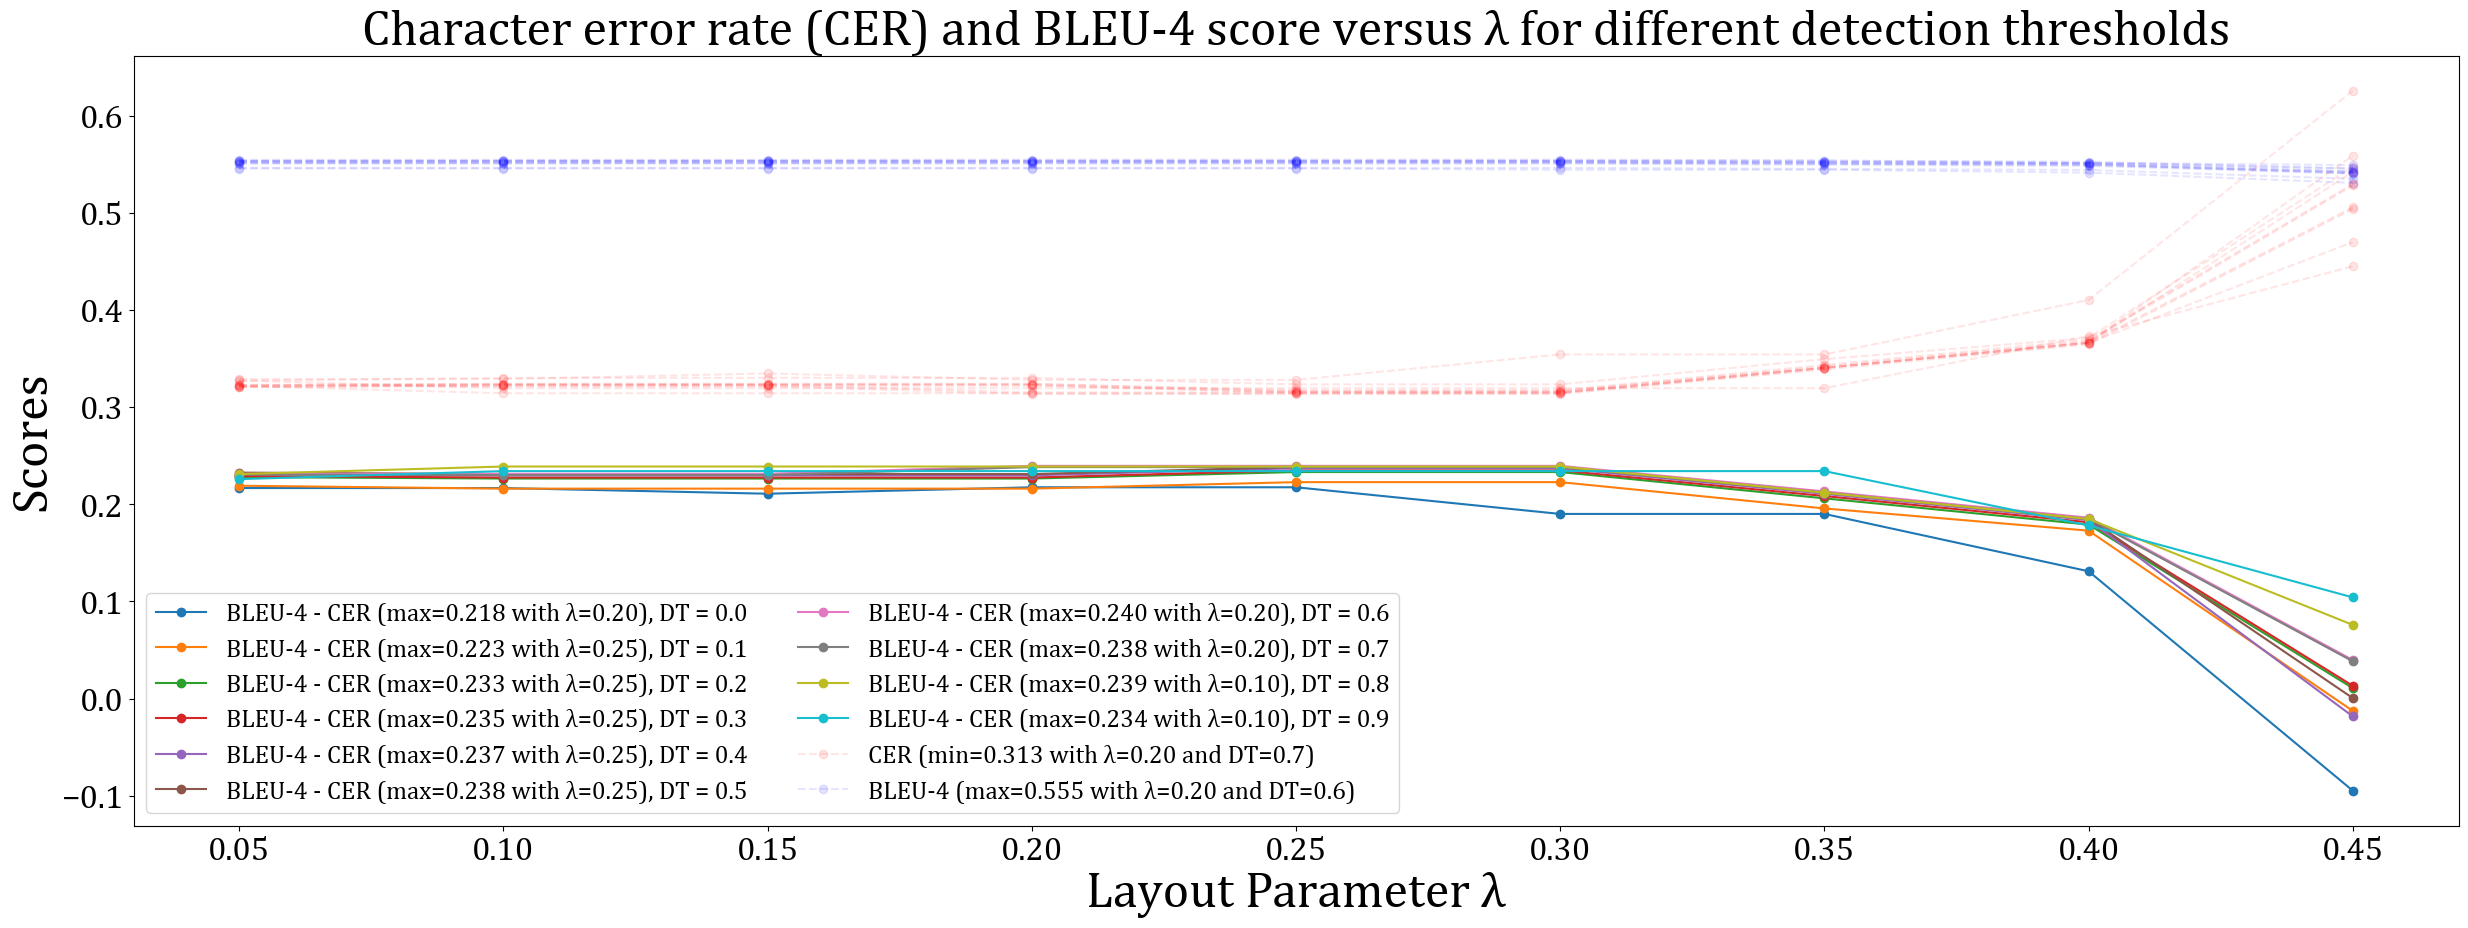
\includegraphics[width=\textwidth]{./figures/cer_bleu.png}
    \caption{Character error rate (CER) and BLEU-4 versus layout parameter $\lambda$ for different detection thresholds, where (BLEU-4 - CER) is used as the primary metric}
    \label{fig:cer_bleu}
\end{figure}

Considering different detection thresholds (DT), it is observed that a higher DT will generally lead to a higher (BLEU-4 - CER) value, which indicates a better balance between character and word level accuracy. This is different to the result in the text detection optimization (Figure \ref{fig:map1}), where the mAP is higher when DT is lower. As the DT trades off precision and recall of the text detection model, this suggests that in the recognition process, the precision of the detection result is more important than the recall. The maximum (BLEU-4 - CER) value (0.24) is achieved at $\lambda=0.2$ and $DT=0.6$, which is selected as the optimal setting for the OCR system. Regarding CER and BLEU-4 independently, the minimum CER (0.313) is achieved at $\lambda=0.2$ and $DT=0.7$, while the maximum BLEU-4 (0.555) is achieved at $\lambda=0.2$ and $DT=0.6$. This indicates that the optimal setting is a trade-off between character and word level accuracy, where the character level accuracy is slightly sacrificed to improve the word and phrase level precision.

\begin{figure}[htbp]
    \centering
    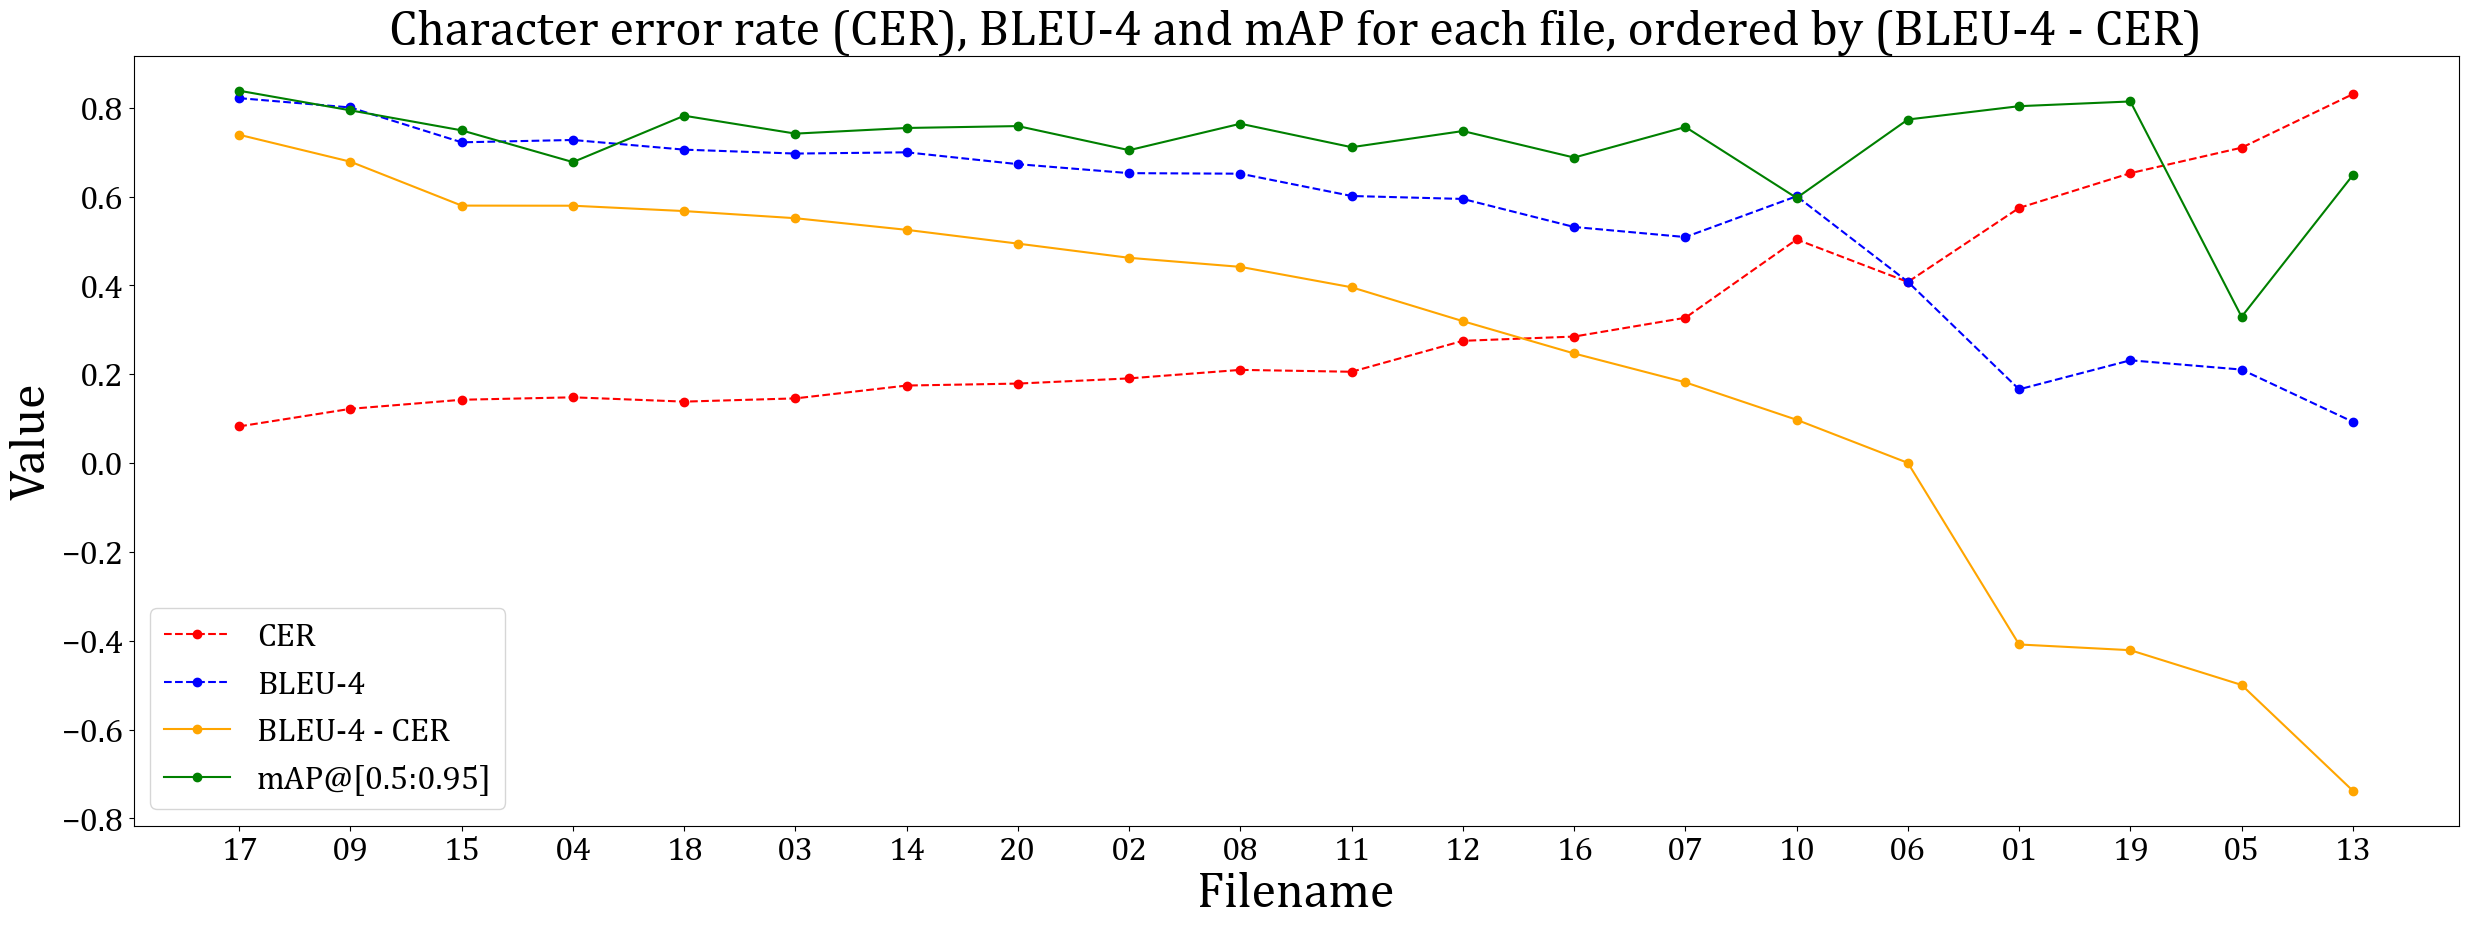
\includegraphics[width=\textwidth]{./figures/cer_bleu_map.png}
    \caption{Character error rate, BLEU-4 and mean average precision for each test image}
    \label{fig:cer_bleu_map}
\end{figure}

Under the optimal settings ($\lambda=0.2$ and $DT=0.6$), we calculated the CER, BLEU-4 and mAP on each test image, as shown in Figure \ref{fig:cer_bleu_map}. We ordered the results by the (BLEU-4 - CER) value for better observation, where the images with higher (BLEU-4 - CER) value are shown at the left. It is observed that the CER and BLEU-4 are generally negatively correlated, where the images with lower CER tend to have higher BLEU-4, and vice versa. This justifies the use of (BLEU-4 - CER) as the primary metric for system optimization. Regarding mAP, we found a weak positive correlation with (BLEU-4 - CER), where the images with higher (BLEU-4 - CER) value tend to have higher mAP, but there are cases where the mAP is high while (BLEU-4 - CER) is low. This indicates that the text detection performance is not the only factor that affects the recognition and ordering performance.

We also noticed that the performance on each file is quite different, where half of the samples achieve $CER<0.2$ and $BLEU>0.65$, which indicates a high-quality recognition result, while the worst sample has $CER>0.8$ and $BLEU<0.1$, which is not acceptable. This suggests that the OCR system can achieve high accuracy on around half of the pages in Funü Zazhi, but may still struggle with some specific pages that are not well covered in the synthetic dataset. We will present some recognition results and analyze common failure cases in Section \ref{sec:discussions}.

\subsection{Confidence Score}
\label{sec:confidence_score}
As discussed in Section \ref{sec:cer_bleu}, the OCR system may not perform well on some pages of Funü Zazhi, where the results are not acceptable. Therefore, we need to filter out these low-quality predictions to avoid introducing noise to the subsequent NLP tasks. To achieve this, we propose to use the confidence score to estimate the accuracy of a prediction, as the ground truth is not available for those images. We investigated the relationship between the CER, BLEU-4 and the following two types of confidence scores for each test image:

\textbf{Text Detection Confidence}: The average confidence score of the detected text lines in the image. The confidence score for each text line is calculated as the maximum probability of the predicted text line by the text detection model. Although it is not directly related to the recognition performance, the quality of the detection result can affect the recognition and ordering performance.

\textbf{Text Recognition Confidence}: The average confidence score of the recognized text lines in the image. The confidence score for each text line is calculated as the average maximum probability of each predicted character in the text line by the text recognition model. This score is more relevant to the recognition performance, as it reflects the accuracy of the recognized text content.

\begin{figure}[htbp]
    \centering
    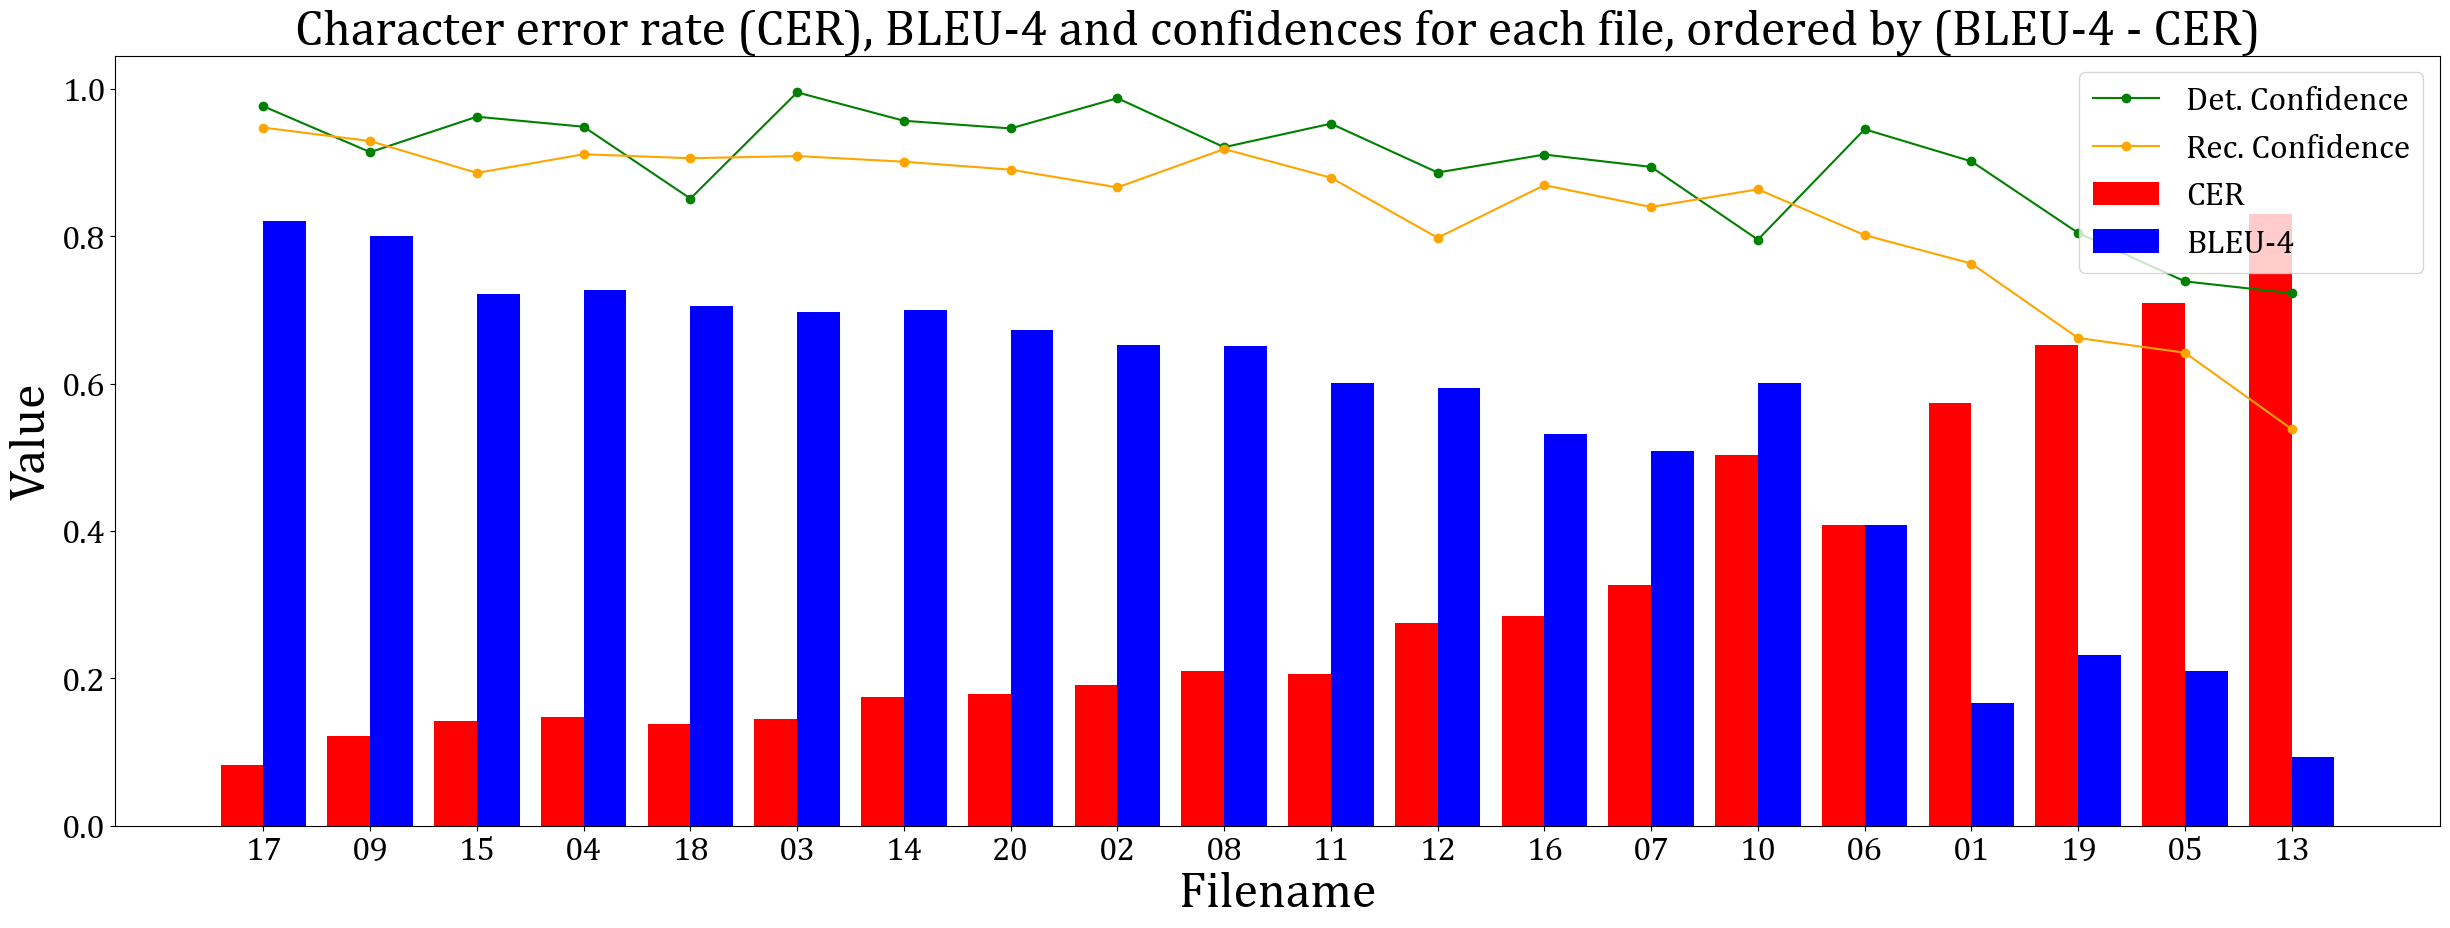
\includegraphics[width=\textwidth]{./figures/cer_bleu_conf.png}
    \caption{Character error rate, BLEU-4 and confidence scores for each test image}
    \label{fig:cer_bleu_conf}
\end{figure}

As shown in Figure \ref{fig:cer_bleu_conf}, we plotted these metrics for each test image in the same order as in Figure \ref{fig:cer_bleu_map}. It is observed that the degree of correlation between (BLEU-4 - CER) and the recognition confidence is higher than the detection confidence, where the images with higher recognition confidence tend to have higher (BLEU-4 - CER) value. This indicates that the recognition confidence is a better estimator for the overall accuracy of the OCR system. We did not combine the two confidence scores as an overall score, as the detection confidence is weakly correlated with the recognition performance, and may introduce noise to the estimation.

\begin{figure}[htbp]
    \centering
    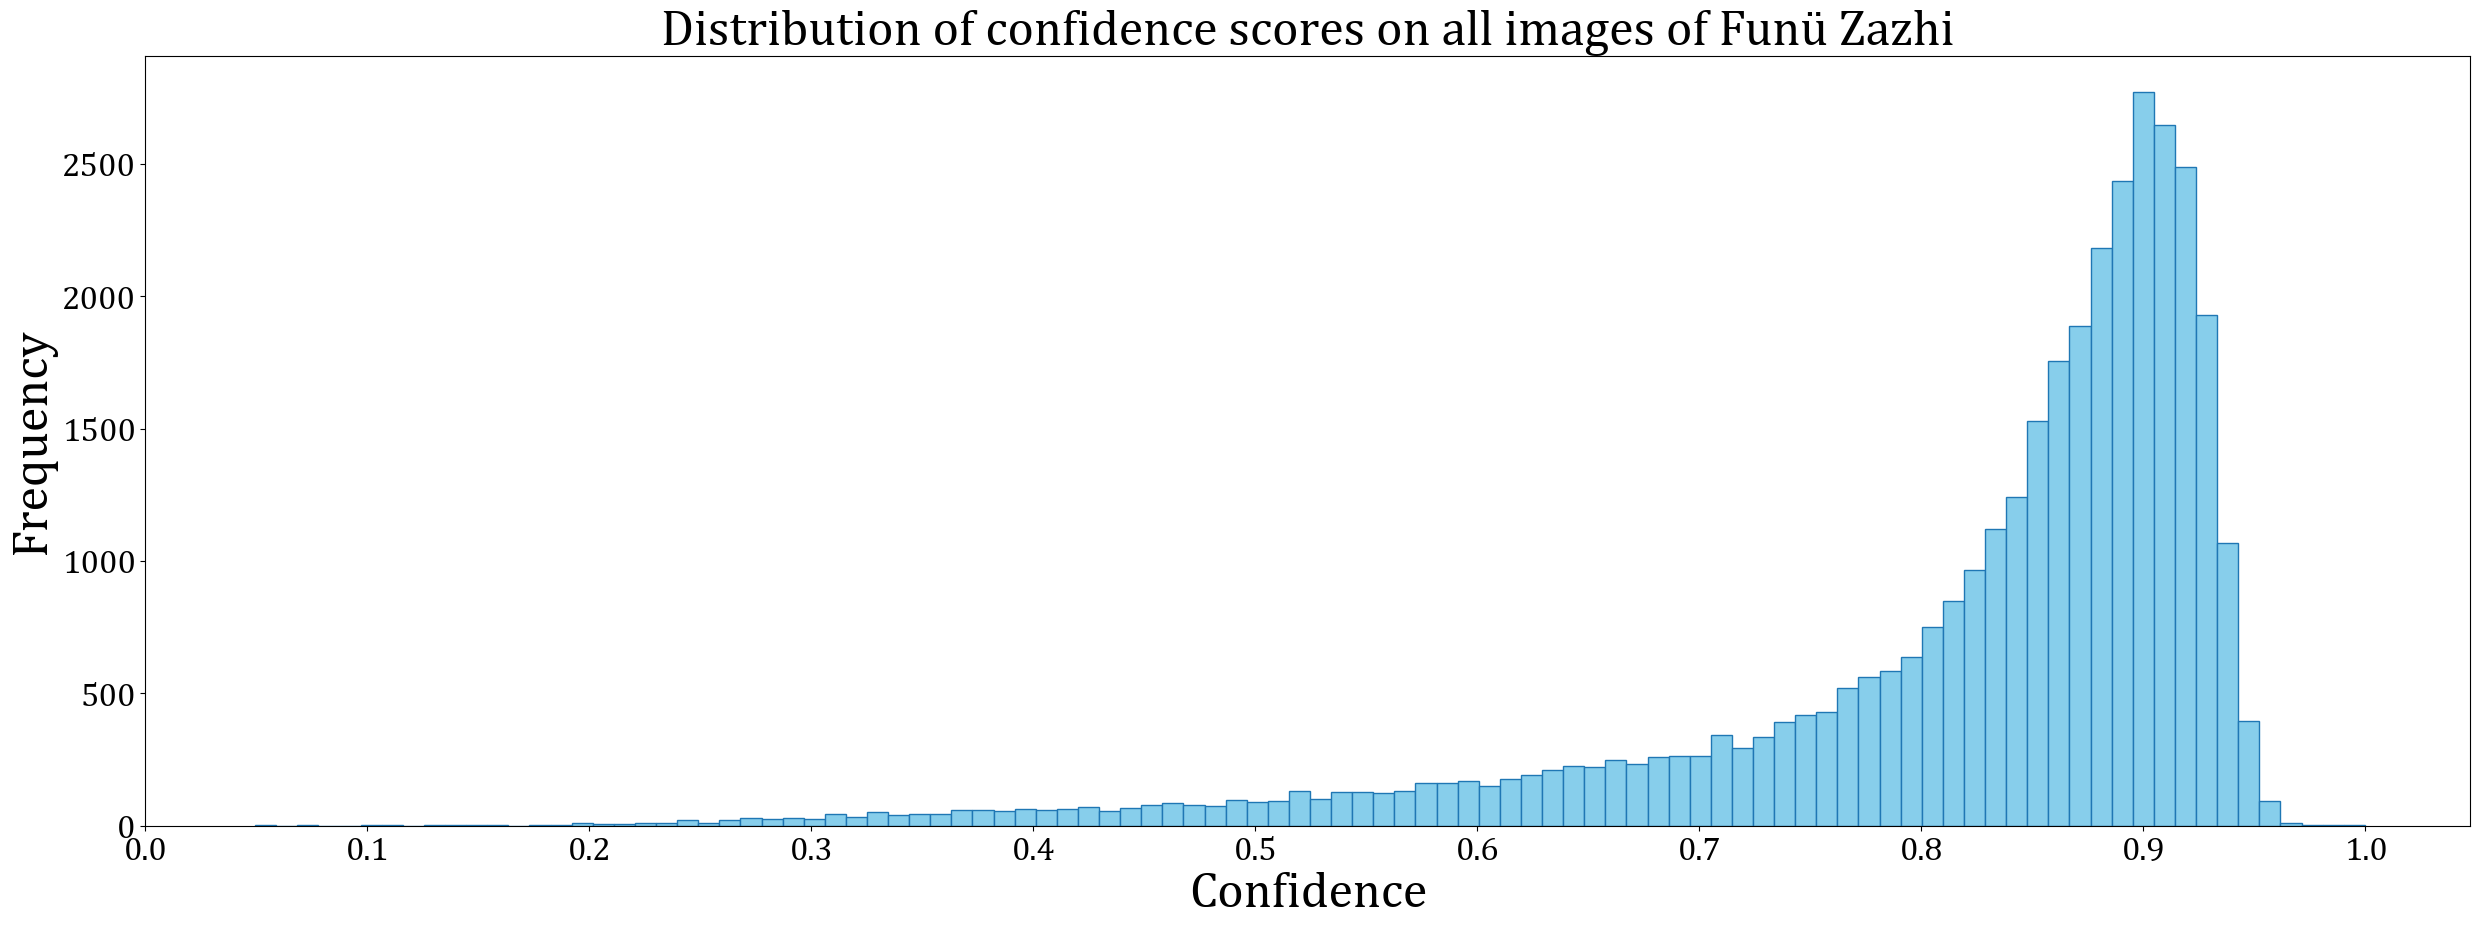
\includegraphics[width=\textwidth]{./figures/confidence1.png}
    \caption{Distribution of confidence scores on all 36,101 images of Funü Zazhi}
    \label{fig:confidence1}
\end{figure}

To further investigate the confidence scores on the whole dataset, we plotted the distribution of recognition confidence on all 36,101 images of Funü Zazhi, as shown in Figure \ref{fig:confidence1}. It is observed that the confidence scores are mostly distributed between 0.8 and 0.95, with a peak around 0.9. Specifically, there are 28\% of images with a confidence score above 0.9, and 72\% above 0.8. In the test set, these two values are 35\% and 75\% respectively, where for images with confidence score above 0.9, the average CER is 0.145, and the average BLEU-4 is 0.729, which is significantly better than the overall average. This indicates that the test set is representative of the whole dataset, and about 30\% of the pages in Funü Zazhi can achieve high-quality recognition results with CER around 0.15 and BLEU-4 around 0.73.

\begin{figure}[htbp]
    \centering
    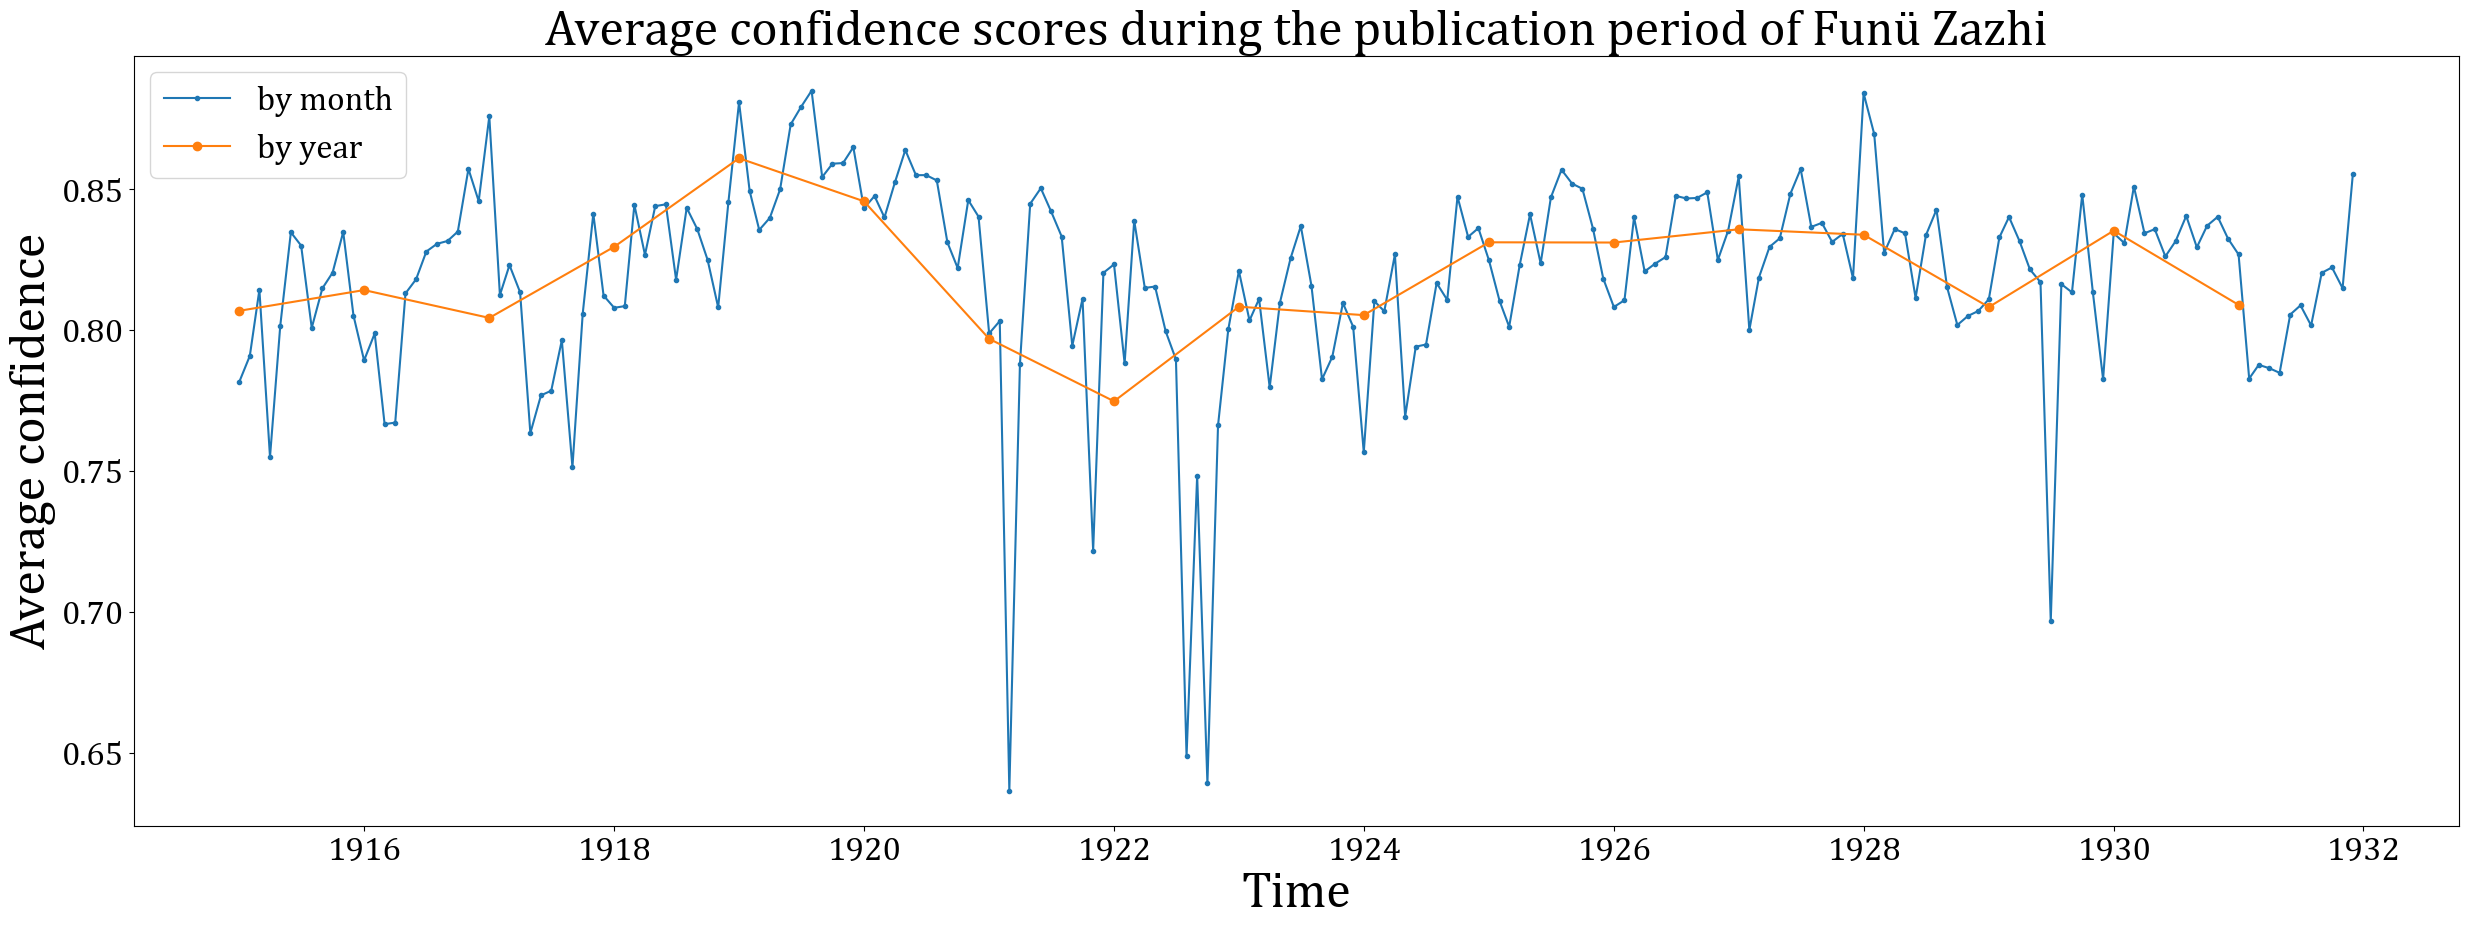
\includegraphics[width=\textwidth]{./figures/confidence2.png}
    \caption{Average confidence scores during the publication period of Funü Zazhi}
    \label{fig:confidence2}
\end{figure}

We also analyzed the average recognition confidence by month or by year during the publication period of Funü Zazhi, as shown in Figure \ref{fig:confidence2}. It is observed that the confidence score fluctuates significantly in the early years, where the average confidence peaks around 0.86 in 1919, and drops to 0.77 in 1922. This indicates that the quality of the scanned images may vary during the publication period, which can affect the recognition performance. The average confidence score for each year stabilizes after 1922 above 0.8, where as the monthly average still fluctuates. The study on confidence scores of all target images provides insights into the dataset quality, and helps to estimate the overall accuracy of the OCR system.

\section{Comparisons}
\label{sec:comparisons}
We compared the performance of our OCR system with four baseline methods, including three open-source OCR tools and a commercial tool, which are state-of-the-art models that support traditional Chinese text recognition. The open-source tools are Tesseract \cite{luscombe2020tesseract}, EasyOCR \cite{easyocr} and PaddleOCR \cite{paddle}, and the commercial tool is Apple MacOS Preview (AMP) \cite{preview}. As a built-in software in MacOS, we can only obtain the recognized text from AMP, while we can obtain other prediction information from the open-source tools, such as text detection bounding boxes. Therefore, AMP is only included in the comparison of text recognition performance.

\begin{table}[htbp]
    \centering
    \begin{tabular}{lcc}
    \toprule
    OCR Method & Total Time (s) & Average Time per File (s) \\
    \midrule
    PaddleOCR & 111.27 & 5.56 \\
    EasyOCR & 104.19 & 5.21 \\
    Tesseract & 71.63 & 3.58 \\
    Ours & 84.85 & 4.24 \\
    Ours (GPU) & \textbf{57.53} & \textbf{2.88} \\
    \bottomrule
    \end{tabular}
    \caption{Comparison of OCR methods based on processing times}
    \label{table:ocr_times}
\end{table}

The comparison is conducted on the test set, where we evaluate the OCR methods based on processing time, mean average precision (mAP), character error rate (CER) and BLEU-4 score. We use default settings and pre-trained models for each baseline method, and the optimal settings for our system as discussed in Section \ref{sec:results}.

The processing time is measured as the total time to recognize all 20 images in the test set, as shown in Table \ref{table:ocr_times}. The result is obtained using Apple M1 chip, and we also tested our system on NVIDIA GeForce GTX 1650 GPU for comparison. We observe that on the M1 chip, the processing speed of our system is slightly slower than Tesseract, but faster than others. While with the GPU, the processing time is significantly reduced to 2.88 seconds per image, which is the shortest among all.

\begin{figure}[htbp]
    \centering
    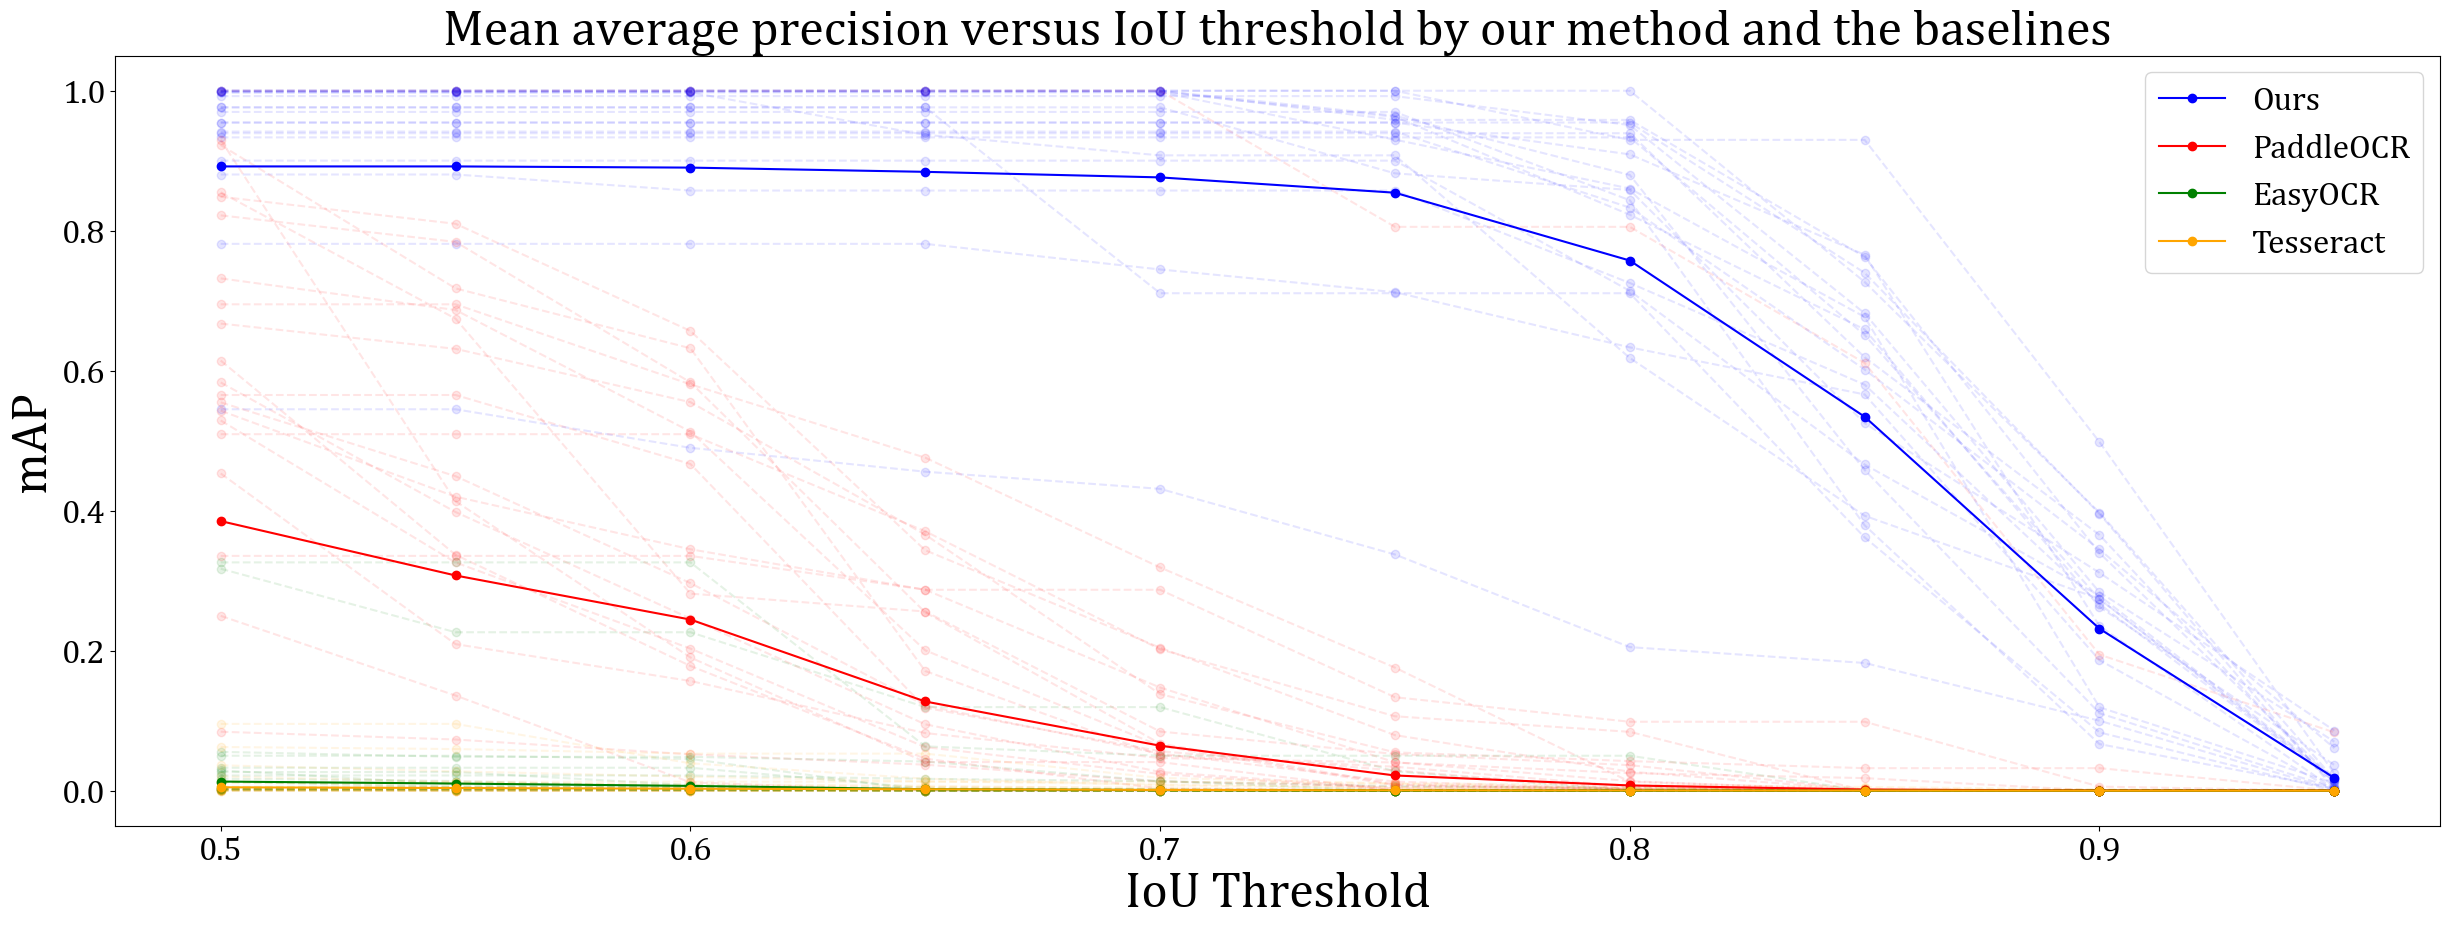
\includegraphics[width=\textwidth]{./figures/comp_map1.png}
    \caption{Comparison of OCR methods on mean average precision versus loUT}
    \label{fig:comp_map1}
\end{figure}

Regarding detection performance, we demonstrate the mAP for each OCR method at different IoU thresholds in Figure \ref{fig:comp_map1}, where the dashed, transclucent lines represent the mAP for a single image, and the solid lines represent the mAP for the whole test set. It is observed that our system achieves a significantly higher mAP at all IoU thresholds than the baselines, which indicates that the text detection model in our system can accurately detect text lines in Funü Zazhi, which is very challenging as the performance of the other methods is quite low.

\begin{figure}[htbp]
    \centering
    \begin{subfigure}[b]{0.23\linewidth}
        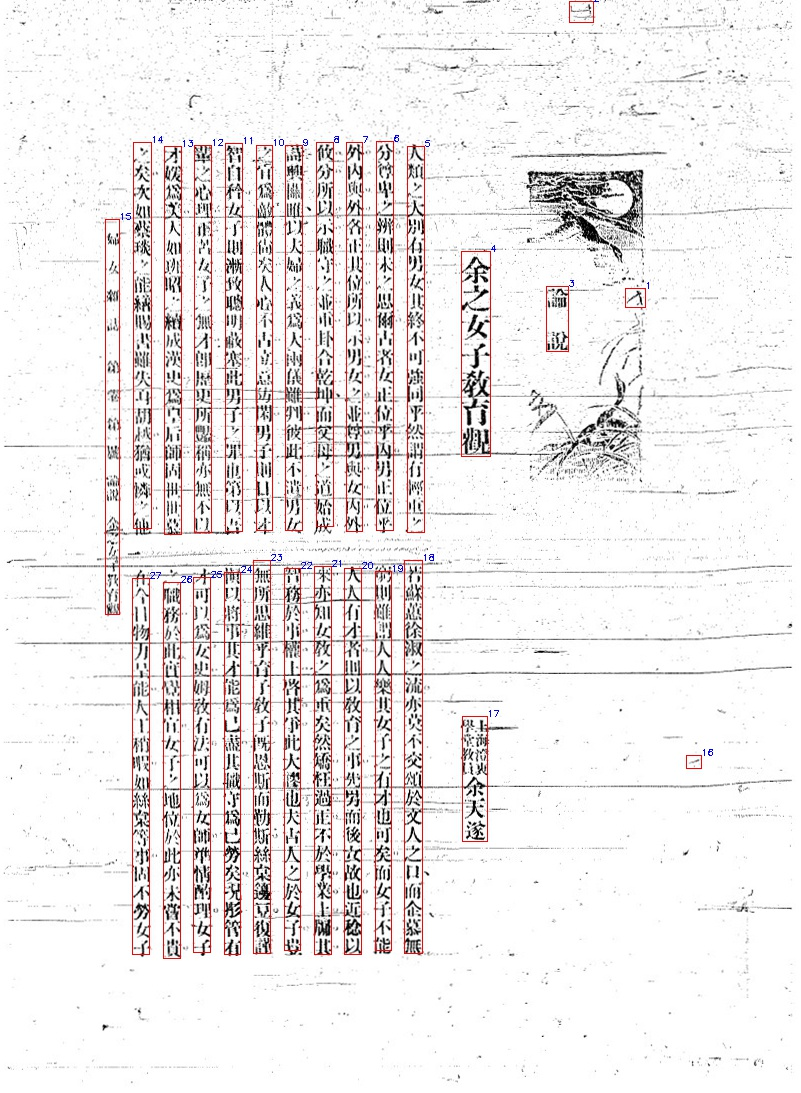
\includegraphics[width=\linewidth]{./figures/samples/ours_01.jpg}
        \caption{Ours}
        \label{fig:ours_01}
    \end{subfigure}
    \hfill
    \begin{subfigure}[b]{0.23\linewidth}
        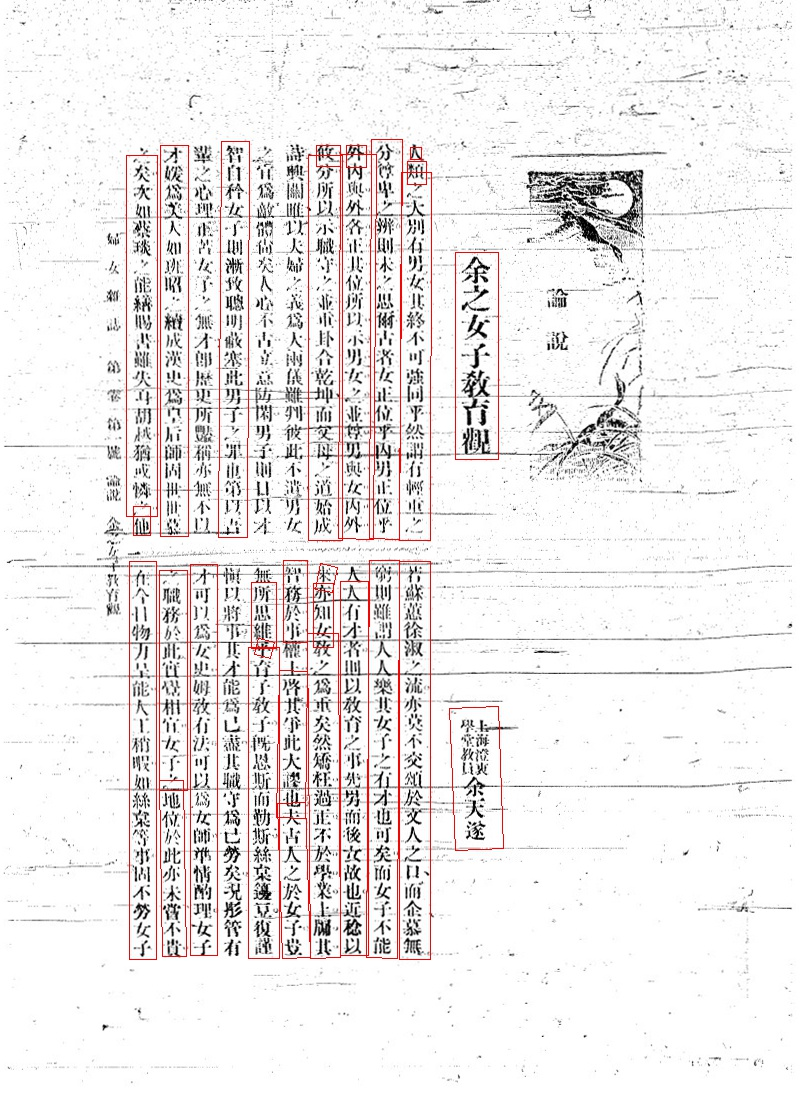
\includegraphics[width=\linewidth]{./figures/samples/paddle_01.jpg}
        \caption{PaddleOCR}
        \label{fig:paddle_01}
    \end{subfigure}
    \hfill
    \begin{subfigure}[b]{0.23\linewidth}
        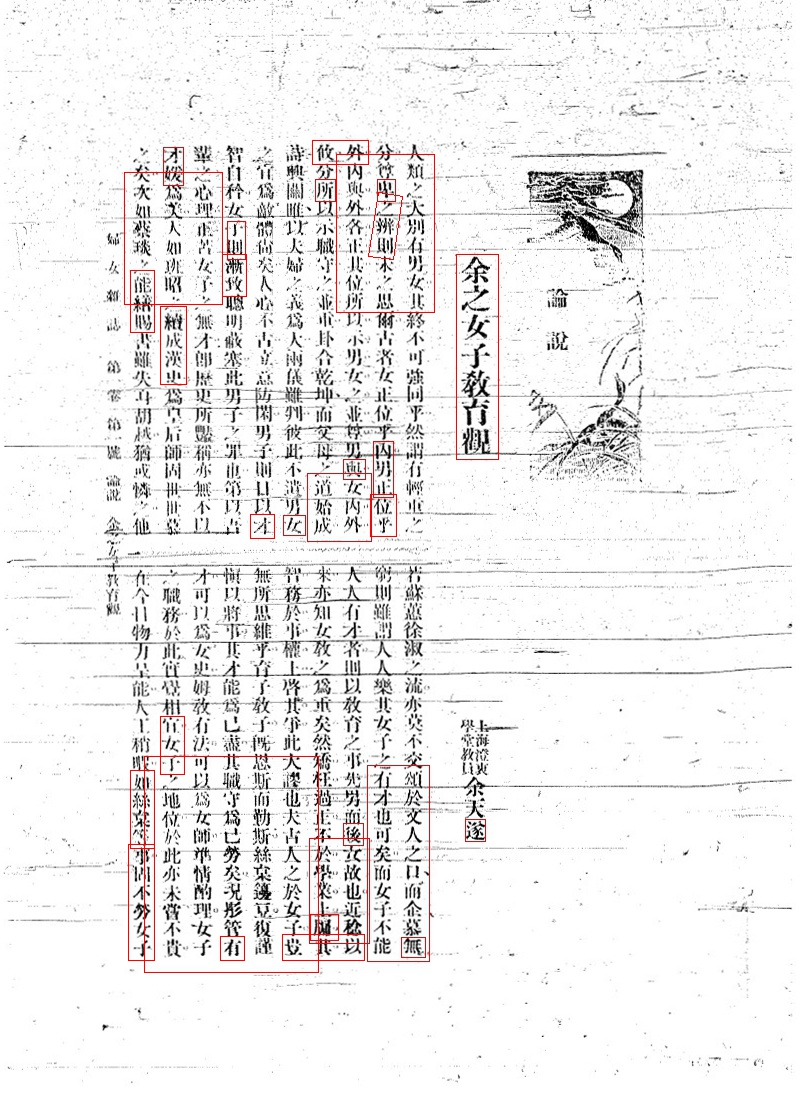
\includegraphics[width=\linewidth]{./figures/samples/easy_01.jpg}
        \caption{EasyOCR}
        \label{fig:easy_01}
    \end{subfigure}
    \hfill
    \begin{subfigure}[b]{0.23\linewidth}
        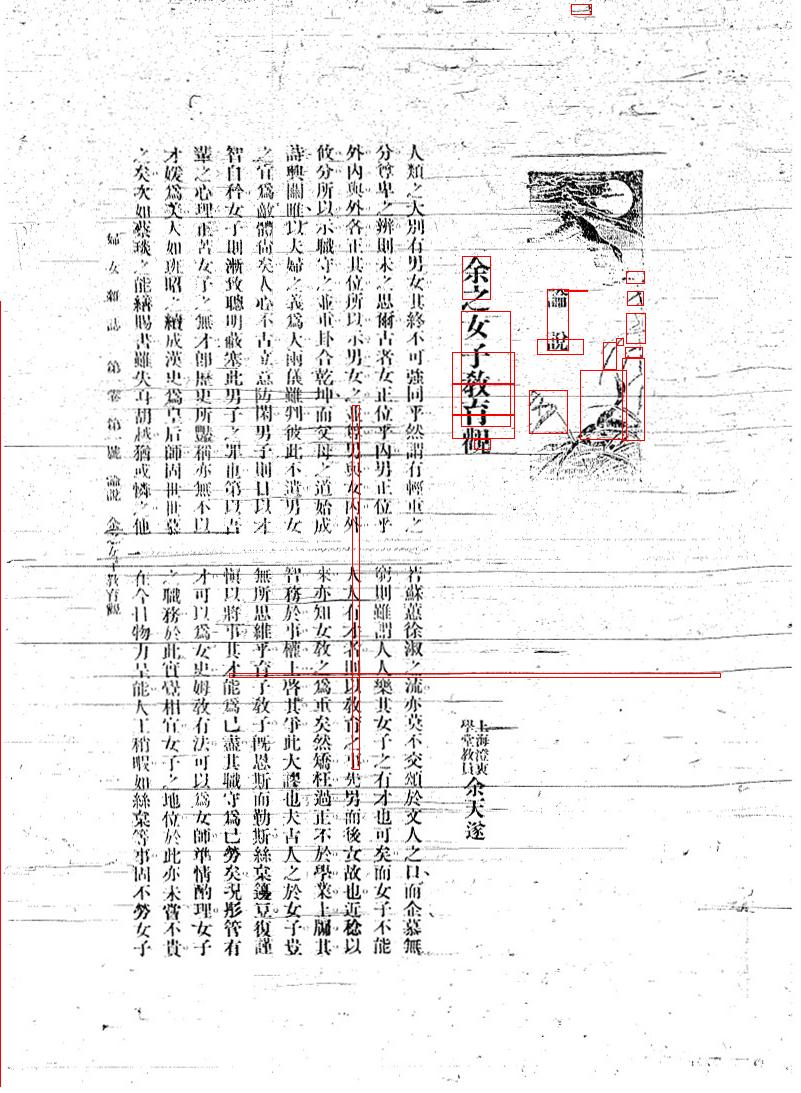
\includegraphics[width=\linewidth]{./figures/samples/tesseract_01.jpg}
        \caption{Tesseract}
        \label{fig:tesseract_01}
    \end{subfigure}
    \caption{Comparison of text detection results on a sample image (filename = 01)}
    \label{fig:detection_compare}
\end{figure}

We visualize the detection results of each OCR method on a sample image (01.jpg in the test set) in Figure \ref{fig:detection_compare}, which represents the typical text layout and average image quality in Funü Zazhi. It is shown that our system can accurately detect all text lines in the image, with very few false predictions. PaddleOCR performs worse with some missing text lines, while EasyOCR and Tesseract have even more false predictions and missing text lines. This indicates that our text detection model can better handle complex background noises that are common in the target dataset, which may confuse other methods.

\begin{figure}[htbp]
    \centering
    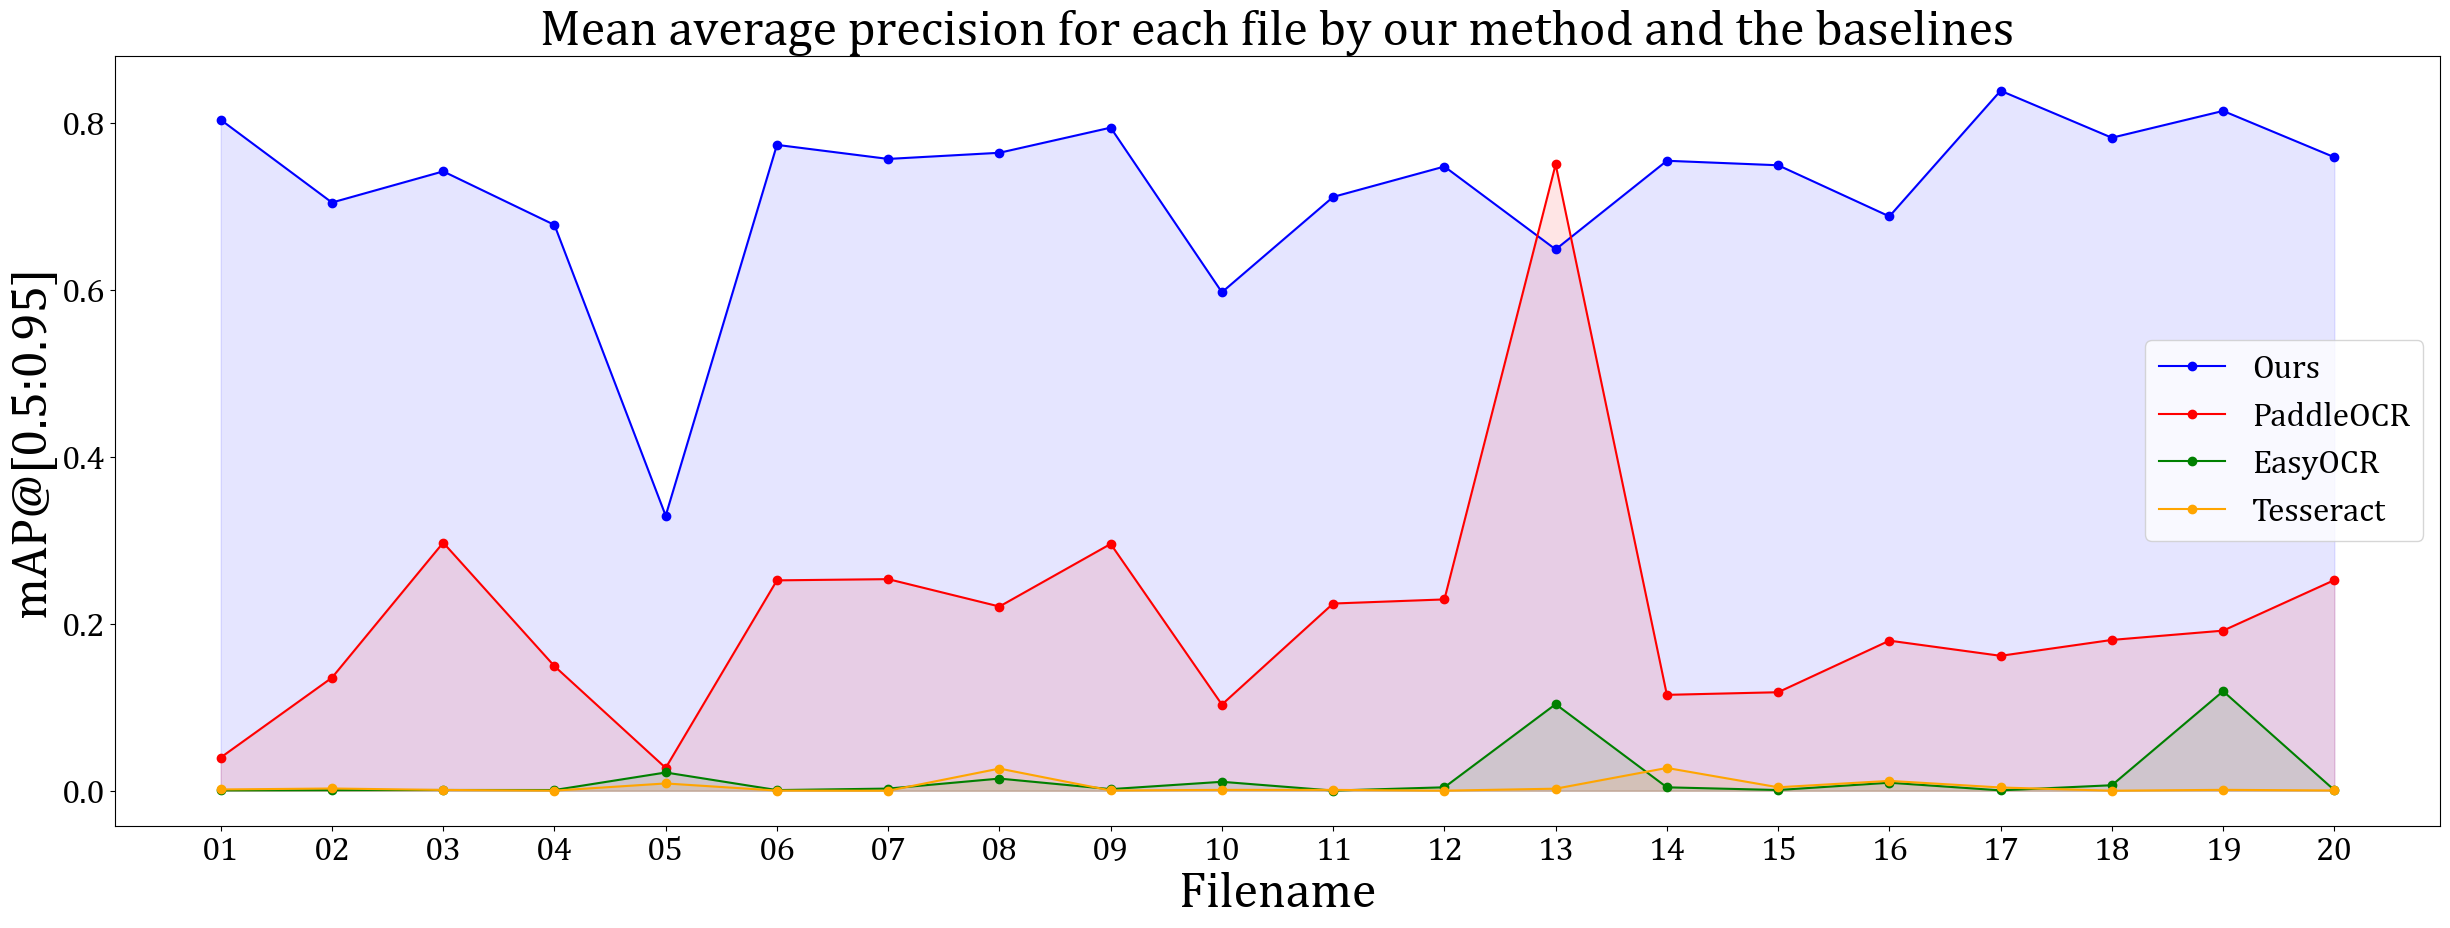
\includegraphics[width=\textwidth]{./figures/comp_map2.png}
    \caption{Comparison of OCR methods on mean average precision for each file}
    \label{fig:comp_map2}
\end{figure}

We also inspected the mAP@[0.5:0.95] for each test image by each OCR method, as shown in Figure \ref{fig:comp_map2}. It is observed that our system achieves the highest mAP on most images, and the result is more stable across different images, which indicates that our system can generalize well to various text layouts in Funü Zazhi. The other methods have more fluctuation in the mAP, suggesting that they may struggle with some specific layouts. We also noticed that the baseline methods perform better on images with many horizontal text lines (e.g., image 13 and 19), which may be because their pre-trained models are optimized for horizontal text detection.

\begin{figure}[htbp]
    \centering
    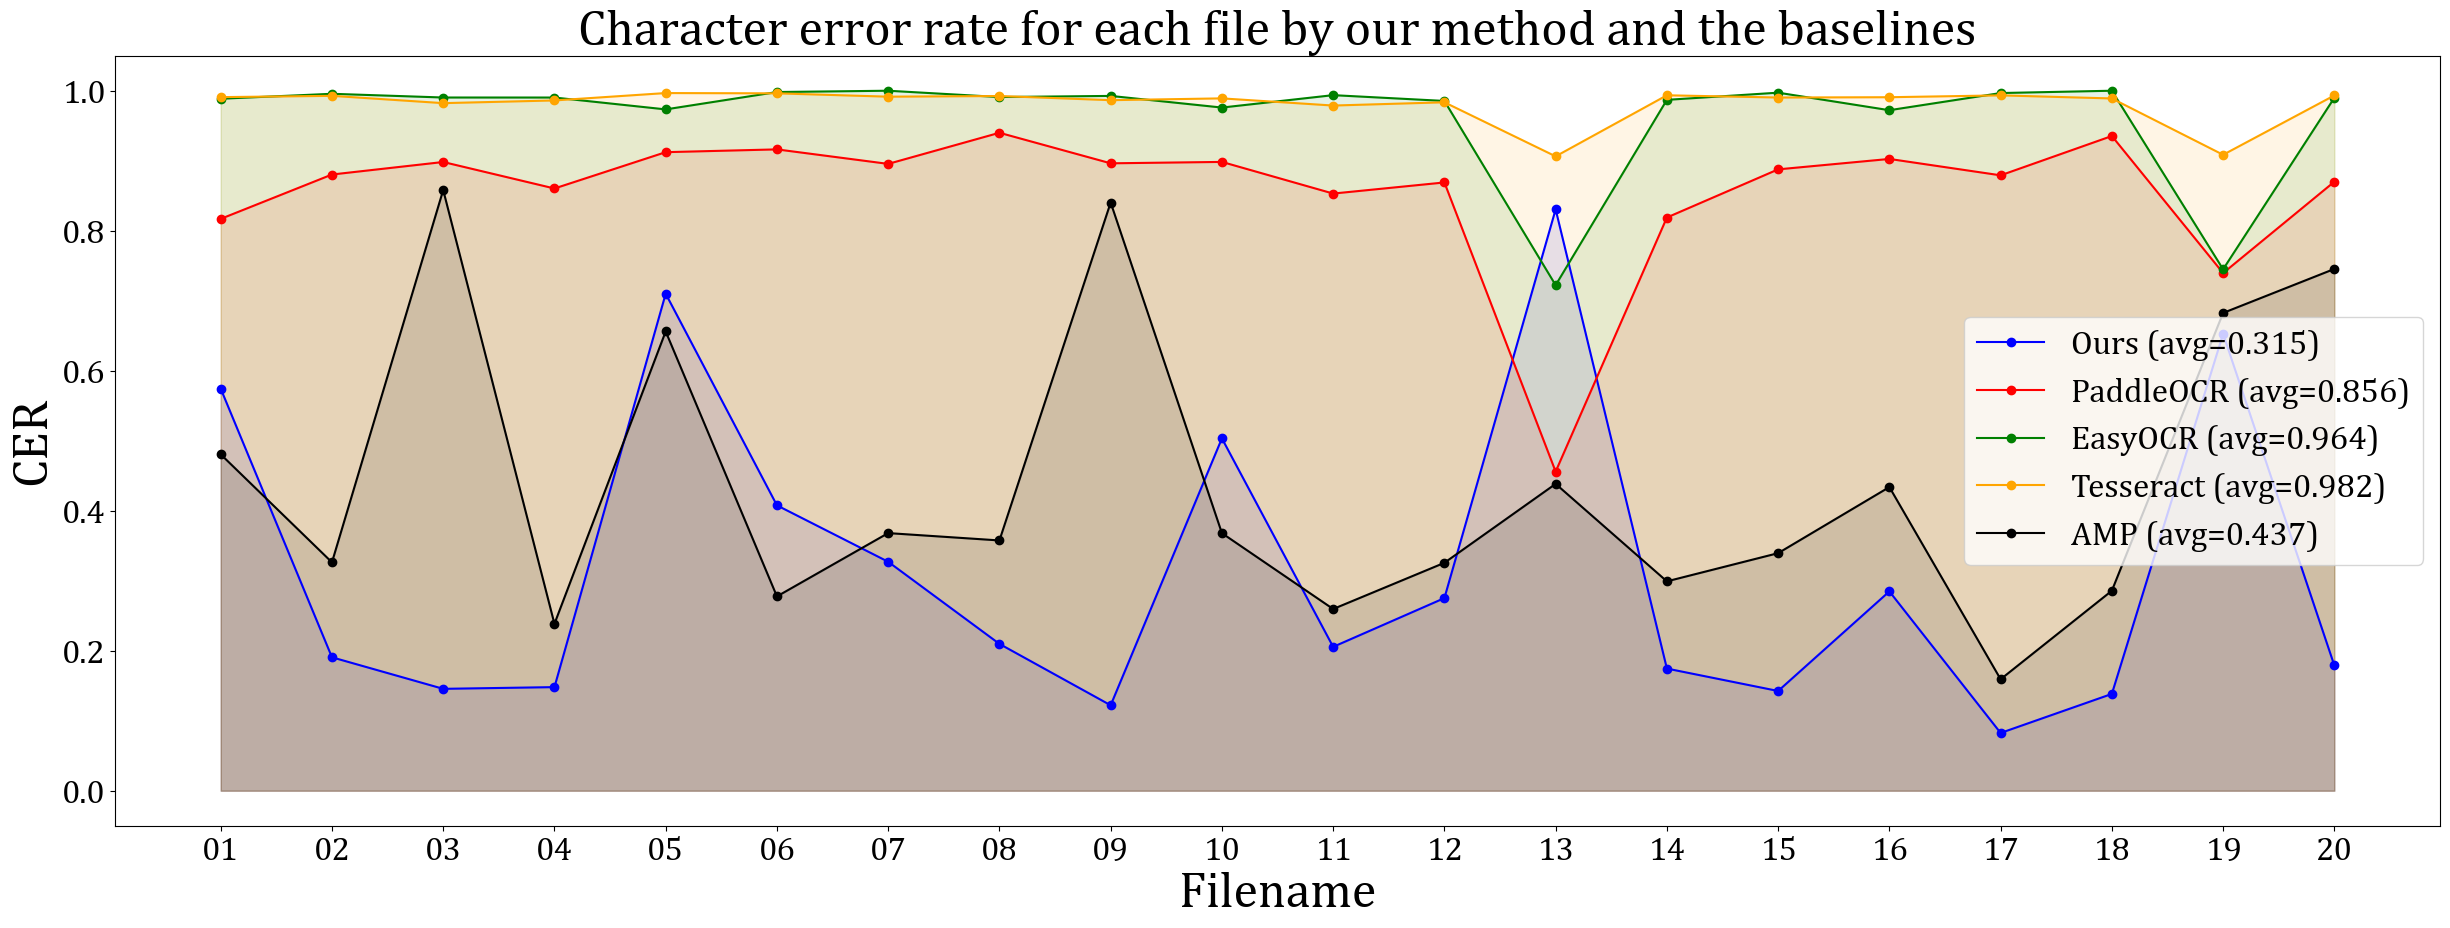
\includegraphics[width=\textwidth]{./figures/comp_cer.png}
    \caption{Comparison of OCR methods on character error rate for each file}
    \label{fig:comp_cer}
\end{figure}

Coonsidering recognition performance, we demonstrate the CER and BLEU-4 for each OCR method on each test image in Figure \ref{fig:comp_cer} and \ref{fig:comp_bleu} respectively. It is shown that the performance of AMP is closer to our system, but our system still achieves a lower CER and higher BLEU-4 to more than 10\% in average. The other baseline methods have a much higher CER and lower BLEU-4 which may due to the poor detection results. The only exception is PaddleOCR, which has a much better BLEU-4 performace than CER, and the reason may be that PaddleOCR fails to order the text lines correctly, which affects the CER but not the BLEU-4.

\begin{figure}[htbp]
    \centering
    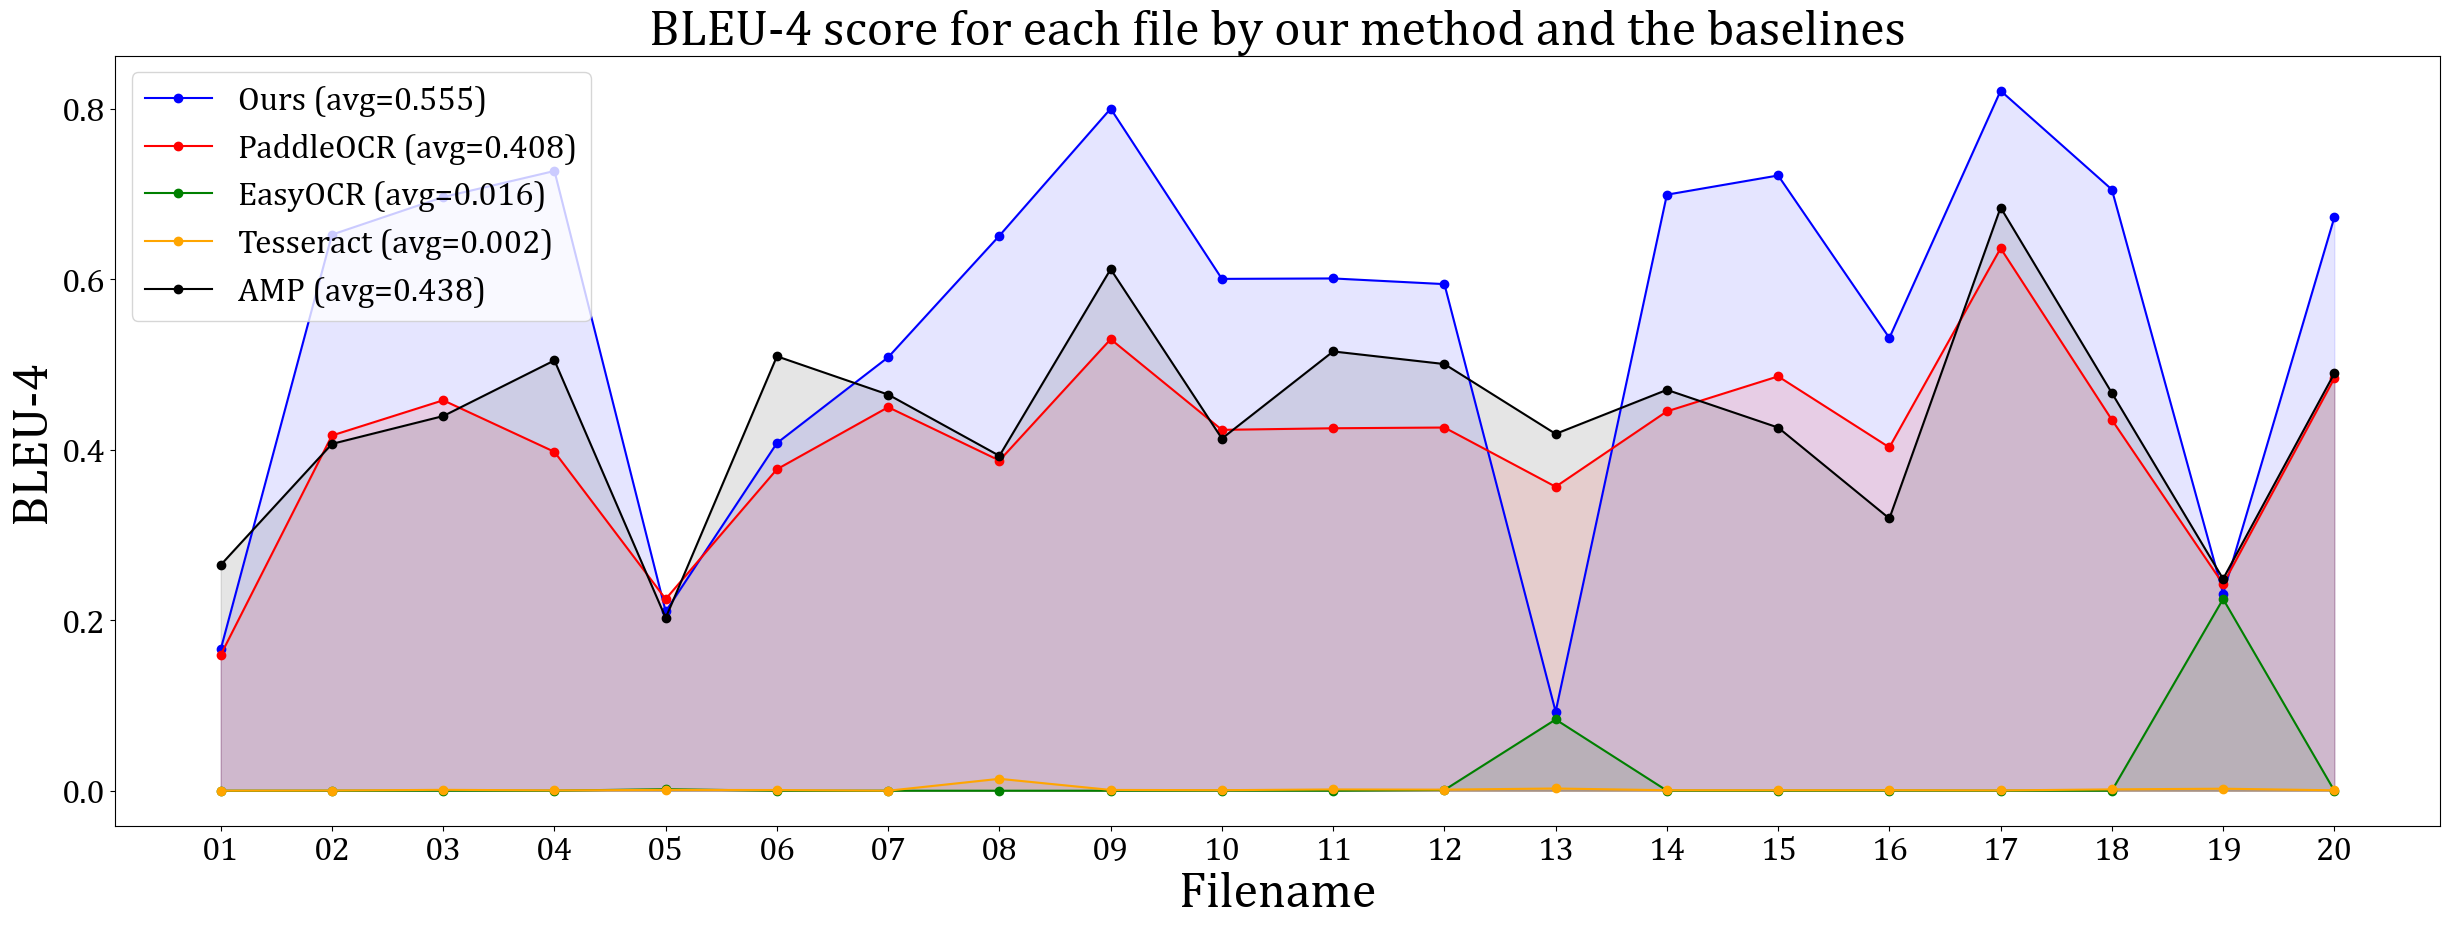
\includegraphics[width=\textwidth]{./figures/comp_bleu.png}
    \caption{Comparison of OCR methods on BLEU-4 score for each file}
    \label{fig:comp_bleu}
\end{figure}

Although our system outperforms other methods in most cases, there are still some images where the recognition performance is not satisfactory and falling behind some baselines, such as image 05 and 13. We will discuss these cases in Section \ref{sec:case_analysis} and analyze the possible reasons. Overall, the comparison results demonstrate that our OCR system can achieve high accuracy on the target dataset, and outperforms the state-of-the-art OCR tools in both text detection and recognition.

\section{Discussions}
\label{sec:discussions}
In this section, we analyze the results of the OCR system on the target dataset, discuss the challenging cases, and identify the limitations of the system.

\subsection{Case Analysis}
\label{sec:case_analysis}
We present some challenging cases to our OCR system in Figure \ref{fig:challenging_cases}, where we show the detection results on the sample images 05, 13 and 19. The performance of our system on these images is not satisfactory, either with a low mAP, a high CER, or a low BLEU-4. We will analyze these cases as follows.

\begin{figure}[htbp]
    \centering
    \begin{subfigure}[b]{0.3\linewidth}
        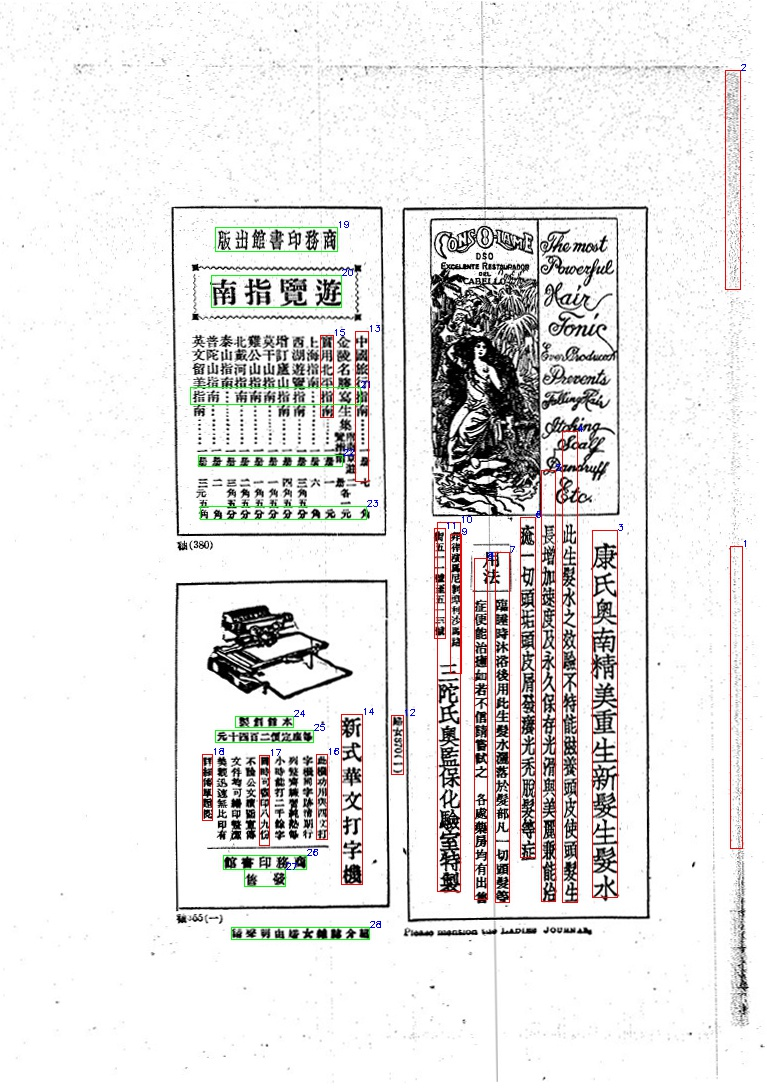
\includegraphics[height=1.35\linewidth]{./figures/samples/05.jpg}
        \caption{05}
        \label{fig:ours_05}
    \end{subfigure}
    \hfill
    \begin{subfigure}[b]{0.3\linewidth}
        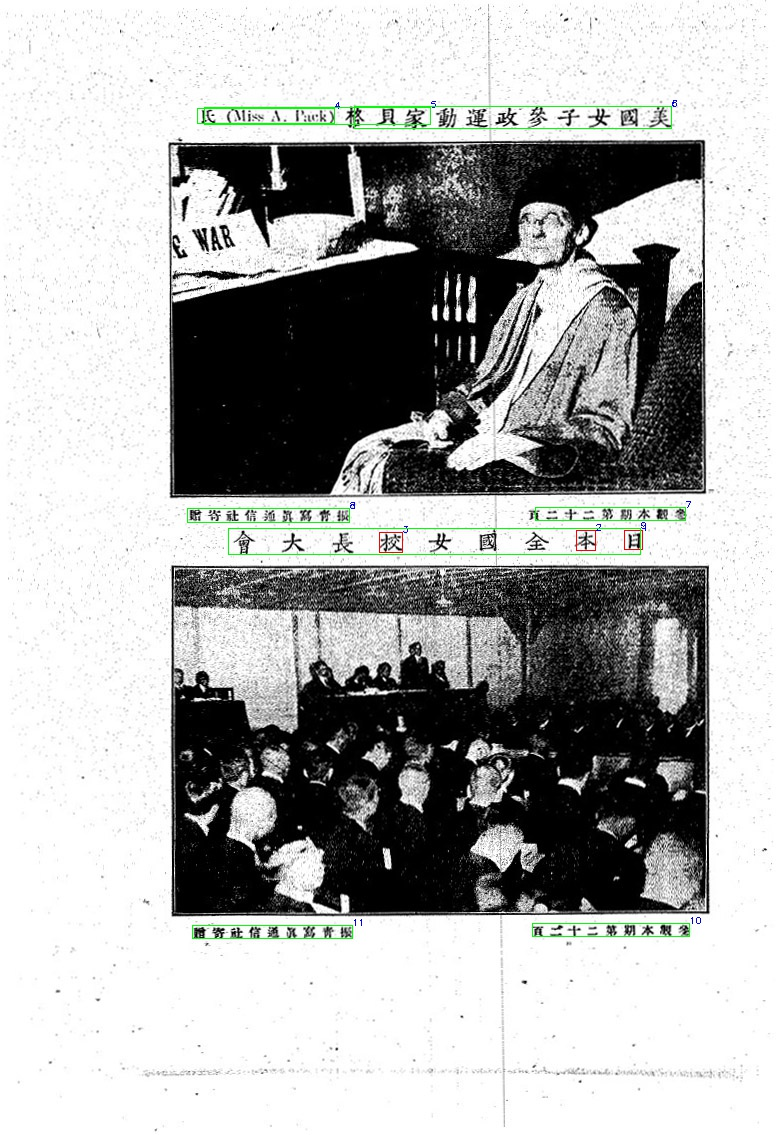
\includegraphics[height=1.35\linewidth]{./figures/samples/13.jpg}
        \caption{13}
        \label{fig:ours_13}
    \end{subfigure}
    \hfill
    \begin{subfigure}[b]{0.3\linewidth}
        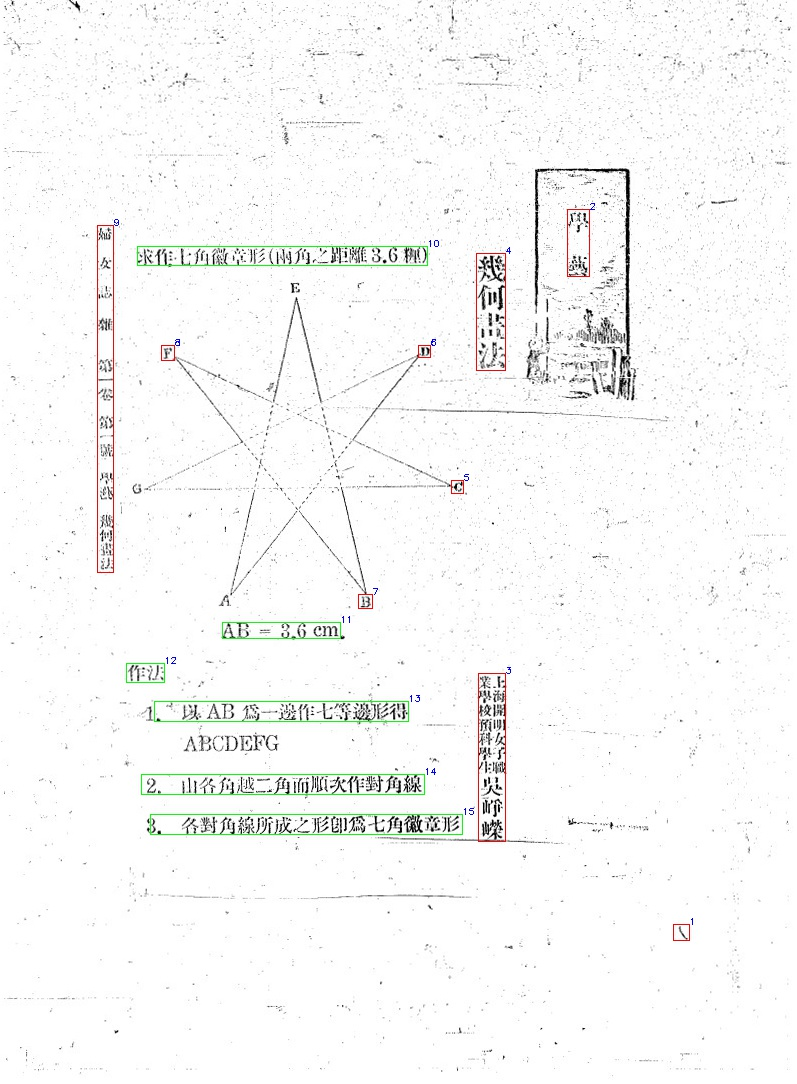
\includegraphics[height=1.35\linewidth]{./figures/samples/19.jpg}
        \caption{19}
        \label{fig:ours_19}
    \end{subfigure}
    \caption{Some challenging cases to our OCR system}
    \label{fig:challenging_cases}
\end{figure}

\textbf{Image 05}: The image has a complex text layout with three blocks and a mix of vertical and horizontal text lines in each block. The text lines are close to each other and have different font sizes, which confuses the text detection model to differentiate between vertical and horizontal lines. As illustrated in Figure \ref{fig:ours_05}, the model takes characters from neighboring vertical lines as part of a horizontal line, which leads to false predictions and missing text lines. As a result, this is the only test image with mAP@[0.5:0.95] below 0.6, and the CER and BLEU-4 are also significantly worse than the average, as shown in Figure \ref{fig:comp_map2}, \ref{fig:comp_cer} and \ref{fig:comp_bleu}. There is also a number of ways to interpret the ground truth text order in this image, which may confuse the text ordering process. The four baseline methods also struggle with this image, where they have a similar or even worse performance than our system.

\textbf{Image 13}: The image has a simple text layout with only horizontal text lines. However, the character spaceing in the middle line is very large, which confuses the text detection model to decide whether recognize the line as a whole or as separate characters, as shown in Figure \ref{fig:ours_13}. Although the detection result is satisfying with no missing lines, the recognition result is the worst in the test set and falls behind 3 baselines, as shwon in Figure \ref{fig:comp_cer} and \ref{fig:comp_bleu}. The reason may be that the text recognition model is not trained to handle such large character spacing, and it is trained with more vertical text lines in the synthetic dataset to match the distribution in Funü Zazhi, which may affect the recognition performance on horizontal lines.

\textbf{Image 19}: The image has a moderate complex text layout with a mix of vertical and horizontal text lines and non-Chinese characters, such as English letters and numbers. As demonstrated in Figure \ref{fig:ours_19}, the detection result in good with only some English letters missing, as we only train the model with Chinese text lines. However, the recognition result is not satisfactory with a high CER and low BLEU-4, as shown in Figure \ref{fig:comp_cer} and \ref{fig:comp_bleu}. The reason may be that the neither the detection nor the recognition models are trained with non-Chinese characters, which makes them unable to extract these text content. The four baseline methods have similar recognition performance on this image although they are multilingual models, which may due to their poor detection results.

In summary, the challenging cases to our OCR system are mainly caused by the complex text layout, the large character spacing, the horizontal text lines, and the non-Chinese characters. The text detection model may struggle with the complex layout and the large spacing, while the text recognition model may struggle with the horizontal lines and the non-Chinese characters. The text ordering process may also be affected by the complex layout. Although these cases are rare in Funü Zazhi, they are still important to consider in the future works.

\subsection{Limitations}
\label{sec:limitations}
We identify several limitations of the OCR system based on the system design, implementation, and evaluation results as follows.

\textbf{Synthetic Data Generation}: The synthetic data generation process is designed to simulate the text layout and content in Funü Zazhi, but it may not cover all possible text layouts and content types. The synthetic image for text detection only simulates two types of the layout, where layout L1 is for the majority in the target dataset, while layout L2 is designed to cover the edge cases by putting text lines randomly. This setting may cover the majority layout better, but may not cover the edge cases well, as a random layout may not represent the real text layout in the target dataset, which has some rules to follow. On the other hand, the synthetic image for text recognition only simulates the Chinese characters, while the target dataset also contains English letters, numbers, and other non-Chinese characters. This setting may help the model generalize well to Chinese characters which is the majority in the target dataset, at the price of poor performance on non-Chinese characters.

\textbf{Text Ordering Algorithm}: The text ordering algorithm is designed to handle the text layout in Funü Zazhi, but it may not cover all possible text layouts. The algorithm works by first distinguish between layout L1 and L2 based on the number of vertical text lines in the upper and lower part of the image, and then order the text lines based on the bounding box coordinates. It works well for layout L1 as the ordering rule is clear, however as there are various ordering rules for the edge cases in layout L2, the general ordering rule in Algorithm \ref{alg:ordering_l2} may not fits them all. In addition, the algorithm is based on the assumption that the text lines are ordered from top to bottom and right to left. Although this is the common rule in the target dataset, there are some cases where the text lines are ordered from left to right, which may confuse the algorithm. The algorithm may also struggle with the text lines that are close to each other, as the bounding box coordinates may not reflect the real order.

\textbf{Generalization Ability}: The OCR system is trained with synthetic data that simulate the characteristics of Funü Zazhi, so it may not generalize well to other kinds of data, such as scene text, handwritten text, or modern-layout documents. Due to the lack of annotated datasets with similar features to Funü Zazhi, it is difficult to train the model with real data, which may help the model generalize better to other datasets. 

\textbf{Training Pipelines}: The training pipelines for text detection and recognition are designed separately, which may not be optimal for the whole OCR system. As the recognition model takes output from the detection model as input, it may be better to train the two models jointly using a single dataset, which can help the models learn the dependencies between the two tasks. It may also be better to integrate a trainable layout classifier into the system before the text ordering process, which may help the system adapt to unusual layouts better than the rule-based classifier.

%%%%%%%%%%%%%%%%%%%%%%%%%%%%%%%%%%%%
\chapter{Conclusion}
\label{sec:conclusion}
This chapter concludes the project by summarizing main contributions, presenting the results, and suggesting future works.

\section{Achievements}
\label{sec:achievements}
To summarize, the main achievements of this project are:

\textbf{OCR System Development}: We developed an OCR system for Funü Zazhi \cite{fnzz}, a historical Chinese magazine with complex page layout, diverse text content, and varying image quality (Section \ref{sec:target_dataset}). The system consists of trainable text detection and recognition models, and a rule-based text ordering algorithm (Section \ref{sec:system_overview}, \ref{sec:ocr_system}).

\textbf{Synthetic Data Generation}: Due to the lack of relevant annotated data, we designed a synthetic data generation process to simulate the text layout and content in Funü Zazhi, which is used to train the text detection and recognition models (Section \ref{sec:synthetic_dataset}). Ablation studies justified the importance of each augmentation technique in the synthetic data generation process (Section \ref{sec:results}).

\textbf{Superior Performance}: The evaluation result shows that the optimal settings can achieve a inference time of 2.88s/image, a mAP@[0.5:0.95] of 0.7, a CER of 0.313, and a BLEU-4 of 0.555 on the test set, outperforming four state-of-the-art OCR tools to a large extent (Section \ref{sec:results}, \ref{sec:comparisons}).

\textbf{Funü Zazhi Digitization}: After converting all 36,101 Funü Zazhi images to text, the confidence scores estimated that about 30\% of them can achieve high-quality recognition results with CER around 0.15 and BLEU-4 around 0.73 (Section \ref{sec:confidence_score}), which is sufficient for the subsequent NLP tasks.

\textbf{User Interface}: We implemented an user interface for the system, which allows users to upload images and view both the detection and recognition results interactively with multiple options (Section \ref{sec:user_interface}).

\section{Future Work}
\label{sec:future_work}
There are several directions for future works to improve the OCR system, based on common practice and the limitations as discussed in Section \ref{sec:limitations}.

\textbf{Real Data Collection}: Collecting more annotated data from Funü Zazhi or similar historical documents can help the system generalize better to the target dataset. The real data can be used to fine-tune the text detection and recognition models, as the synthetic data may not cover all possible text layouts and content types.

\textbf{Text Ordering}: Designing a trainable, more flexible text ordering model that can handle various text layouts in Funü Zazhi will improve the quality of the final output. The model can be trained with real data to learn the relationship between text lines, and output their reading order directly based on their bounding boxes, which may be more accurate than the rule-based algorithm.

\textbf{Synthetic Data Generation}: Improving the synthetic data generation process to cover more possible text layouts and content types. This may include setting more rules for layout L2, simulating non-Chinese characters in the recognition dataset, and adding more noise types to the synthetic images.

\textbf{Model Integration}: Integrating the text detection, recognition, and ordering models into a single pipeline, and training them jointly using a single dataset. This may help the models learn the dependencies between the tasks to improve the performance.

\textbf{Further Evaluation}: Conducting further evaluations on the OCR system with more test images and SOTA tools. This may help us better understand the performance and identify the limitations of our system. The evaluation can also be conducted on other historical Chinese magazines to test the generalization ability of the system.

\textbf{Usage Extension}: Extending the usage of the OCR system to digitize other historical Chinese documents. This may require fine-tuning the models with more annotated data from different sources to adapt to the new dataset, and designing a more flexible text ordering algorithm to handle various text layouts.

\textbf{User Interface}: Improving the user interface by adding more features, such as batch processing, text editing, and text searching. This may help users to process multiple images, correct recognition errors, and locate specific text content in the image.

\textbf{Deployment}: Deploying the OCR system as a web application or a desktop application, which can be used by researchers, librarians, and historians to extract text content from historical documents. The application can be integrated with other NLP tools to perform more advanced analysis on the text content.

%%%%%%%%%%%%%%%%%%%%%%%%%%%%%%%%%%%%
\begin{appendices}
\chapter{User Manual}
\label{app:user_manual}
The user manual provides a step-by-step guide on how to use the OCR system, including the project structure, the installation process and the system usage. The manual is also available in the README file of the project repository \cite{gitlab}.

\section{Project Structure}
\label{sec:project_structure}
The project root directory is structured as follows:

{\fontsize{10pt}{10pt}\selectfont
\begin{itemize}[leftmargin=*]
    \item \texttt{data/}: Contains files for generating the synthetic dataset (Section \ref{sec:synthetic_dataset}).
    \item \texttt{models/}: Contains the pre-trained models for text detection and recognition (Section \ref{sec:ocr_system}).
    \item \texttt{notebooks/}: Contains the Jupyter notebooks for experiments and evaluation (Section \ref{sec:experiments} to \ref{sec:comparisons}).
    \begin{itemize}
        \item \texttt{confidence.ipynb}: Plot the confidence scores on the target dataset (Figure \ref{fig:confidence1}, \ref{fig:confidence2}).
        \item \texttt{crnn\_rec.ipynb}: Train the CRNN model for text recognition (Section \ref{sec:text_recognition_training}).
        \item \texttt{eval\_comp.ipynb}: Compare the system performance with baselines (Figure \ref{fig:comp_map1} to \ref{fig:comp_bleu}).
        \item \texttt{fnzz.ipynb}: Analyze the Funü Zazhi dataset (Figure \ref{fig:fnzz1}, \ref{fig:fnzz2}).
        \item \texttt{frcnn\_det.ipynb}: Train the Faster R-CNN model for text detection (Section \ref{sec:text_detection_training}).
        \item \texttt{utils.ipynb}: Run utility functions for the experiments.
    \end{itemize}
    \item \texttt{output/}: Contains the output files from the OCR models in experiments (Section \ref{sec:experiments}).
    \begin{itemize}
        \item \texttt{samples/}: Contains the OCR output of 20 test images.
        \item \texttt{images/,positions/,raw/,text/}: Contains the image (with boxes) / positions / raw JSON data / text output from the OCR system on all target images (to be obtained by \texttt{predict.py}).
        \item \texttt{confidence.csv}: Contains the confidence scores of the OCR system on all target images.
    \end{itemize}
    \item \texttt{plots/}: Contains the plots generated in the experiments (Section \ref{sec:results}).
    \item \texttt{reports/}: Contains the source code, figures or PDFs for all project reports.
    \item \texttt{slides/}: Contains the source code, figures and PDF for presentation.
    \item \texttt{src/}: Contains the source code for the project.
    \begin{itemize}
        \item \texttt{app.py}: Run the user interface of the OCR system (Section \ref{sec:user_interface}).
        \item \texttt{compare.py}: Utility functions for comparing the system with baselines (Section \ref{sec:comparisons}).
        \item \texttt{convert.py}: Convert the original text output from traditional Chinese to simplified Chinese.
        \item \texttt{dataset.py}: Create an image dataset of 6,000 Chinese characters in 12 fonts.
        \item \texttt{download.py}: Download the Funü Zazhi dataset, including the images and table of contents.
        \item \texttt{evaluate\_det.py}: Evaluate the text detection model and output Figure \ref{fig:map2}, \ref{fig:map3}.
        \item \texttt{evaluate\_rec.py}: Evaluate the text recognition model and output Figure \ref{fig:cer_bleu_map}, \ref{fig:cer_bleu_conf}.
        \item \texttt{hp\_tuning.py}: Perform hyperparameter tuning for the system and output Figure \ref{fig:map1}, \ref{fig:cer_bleu}.
        \item \texttt{model.py}: Define the deep learning models in the OCR system (Section \ref{sec:ocr_system}).
        \item \texttt{predict.py}: Perform our OCR methods on the images and save the output (Section \ref{sec:system_usage})
        \item \texttt{sort.py}: Sort the output text data of Funü Zazhi by content type, publication date, and confidence scores and save to different folders (Section \ref{sec:system_usage}).
        \item \texttt{table.py}: Extract data from the table of contents downloaded by \texttt{download.py}, which contains the content type and title for each image, and save to a CSV file (Section \ref{sec:system_usage}).
        \item \texttt{utils.py}: Utility functions for the system, such as data processing, image visualization, and evaluation metrics.
        \item \texttt{easy\_ocr.py,paddle\_ocr.py,tesseract\_ocr.py}: Perform EasyOCR / PaddleOCR / Tesseract on the test images and save the output to \texttt{output/samples/}.
    \end{itemize}
    \item \texttt{target/}: Contains the images (to be downloaded) of Funü Zazhi, and annotated test images.
    \begin{itemize}
        \item \texttt{samples/}: Contains the 20 annotated test images for evaluation.
        \item \texttt{tables/}: Contains the table of contents of Funü Zazhi (downloaded by \texttt{download.py}).
        \item \texttt{data\_raw.csv,data.csv}: The output of \texttt{table.py} which contains the content type and title for each image labelled as \texttt{yymm\_xxxx} (Section \ref{sec:target_dataset}).
    \end{itemize}
\end{itemize}}

\section{Installation}
\label{sec:installation}
To run the OCR system, you need to install Python and relevant packages as follows:

\begin{lstlisting}[language=bash]
# Clone the repository
git clone https://gitlab.doc.ic.ac.uk/ms423/msc-individual-project.git

# Navigate to the project directory
cd msc-individual-project

# Create a virtual environment (optional but recommended)
python -m venv venv
source venv/bin/activate # Linux / MacOS
venv\Scripts\activate # Windows

# Install the required packages
pip install -r requirements.txt
\end{lstlisting}

The 20 test images are provided in the \texttt{target/samples/} directory. You can also download the whole Funü Zazhi dataset by running the following command:

\begin{lstlisting}[language=bash]
python src/download.py -i
\end{lstlisting}

The downloaded images will be saved in the \texttt{target/images/} directory. Depending on the network speed, the download process may take several hours. The table of contents of Funü Zazhi is also provided in \texttt{target/data.csv}, which is used to sort the text content by type in \texttt{sort.py}, as discussed in Section \ref{sec:system_usage}.

\section{System Usage}
\label{sec:system_usage}
\subsection{Text Detection and Recognition}
To run the OCR system on the target images, you can use \texttt{predict.py} as follows:

\begin{lstlisting}[language=bash]
# Perform OCR on the whole dataset (assume downloaded)
python src/predict.py

# Perform OCR on the 20 test images
python src/predict.py -t

# Perform OCR on the whole dataset and overwrite the existing output
python src/predict.py -o

# Perform OCR on the 20 test images and overwrite the existing output
python src/predict.py -t -o
\end{lstlisting}

The output of the OCR system will be saved in the \texttt{output/} directory if using the whole dataset, or in the \texttt{output/samples/} directory if using the test images. By default, the output only include the JSON files of the text detection and recognition results. If you want to include other output files, such as the ordered text content, the positions of the text lines, or the image with bounding boxes, you can set the corresponding flags in \texttt{predict.py}:

\begin{lstlisting}[language=python]
output_raw = True # Save the raw JSON data

output_text = True # Save the ordered text content

output_positions = True # Save the positions of the text lines

output_image = True # Save the image with bounding boxes
\end{lstlisting}

After obtaining the text content of Funü Zazhi, you can convert the traditional Chinese characters to simplified Chinese by running the following command:

\begin{lstlisting}[language=bash]
python src/convert.py
\end{lstlisting}

The converted text content will be saved in the \texttt{output/text\_simplified/} directory. You can also sort the text content by content type, publication date, and confidence scores by running the following command:

\begin{lstlisting}[language=bash]
python src/sort.py
\end{lstlisting}

The sorted text content will be saved in the \texttt{text\_sorted\_type/}, \texttt{text\_sorted\_year/}, and \texttt{text\_sorted\_confidence/} subdirectories in the \texttt{output/} directory respectively.

To start the user interface of the OCR system, you can run the following command:

\begin{lstlisting}[language=bash]
python src/app.py
\end{lstlisting}

The user interface will display shortly. You may follow the buttons and checkboxes to upload images and view the detection and recognition results in different options. The detailed demonstration of the user interface is provided in Section \ref{sec:user_interface}.

\subsection{Training and Evaluation}
To train the text detection and recognition models, you first need to create an image dataset of 6,000 Chinese characters in 12 fonts by running the following command:

\begin{lstlisting}[language=bash]
python src/dataset.py
\end{lstlisting}

The dataset will be saved in the \texttt{data/train\_6k/} directory. You can then train the text detection and recognition model in the \texttt{notebooks/frcnn\_det.ipynb} and \texttt{notebooks/crnn\_rec.ipynb} respectively, following the steps there.

To evaluate the text detection and recognition models and showing hyperparameter tuning results, you can run the following commands:

\begin{lstlisting}[language=bash]
# Evaluate the text detection model
python src/evaluate_det.py

# Evaluate the text recognition model
python src/evaluate_rec.py

# Demonstrate the hyperparameter tuning results
python src/hp_tuning.py
\end{lstlisting}

The relevant plots will be saved in the \texttt{plots/} directory. To perform OCR using the baseline methods, you can run the following commands:

\begin{lstlisting}[language=bash]
# Perform EasyOCR on the 20 test images
python src/easy_ocr.py

# Perform PaddleOCR on the 20 test images
python src/paddle_ocr.py

# Perform Tesseract on the 20 test images
python src/tesseract_ocr.py
\end{lstlisting}

The output of the baseline methods will be saved in the \texttt{output/samples/} directory. You can then compare the system with the baselines in \texttt{notebooks/eval\_comp.ipynb}. The results of these experiments are provided in Section \ref{sec:results} and \ref{sec:comparisons}.

\chapter{Test Images}
\label{app:test_images}
The 20 annotated test images used in the evaluation of the OCR system are provided in this appendix. The images are named as \texttt{01.jpg} to \texttt{20.jpg}, and are saved in the \texttt{target/samples/images/} directory. The images are in JPEG format with a resolution of roughly 750 $\times$ 1000 pixels, and are annotated with the text content and positions in the \texttt{target/samples/text/} and \texttt{target/samples/positions/} directories respectively.

\begin{figure}[htbp]
    \centering
    \begin{subfigure}[b]{0.23\linewidth}
        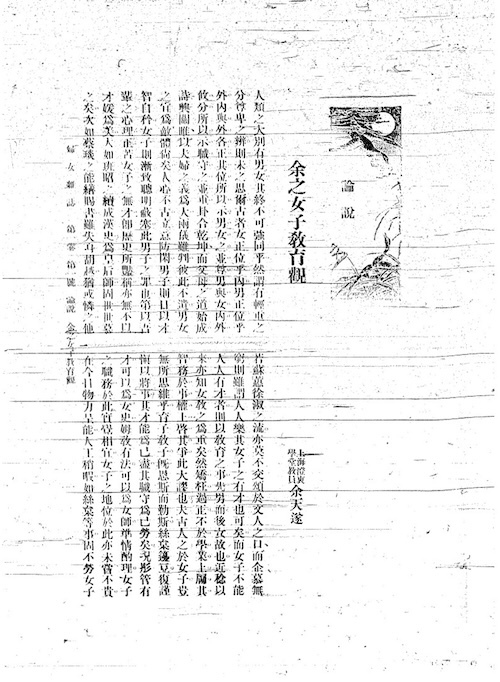
\includegraphics[width=\linewidth]{./figures/testset/01.jpg}
        \caption{01}
        \label{fig:test_01}
    \end{subfigure}
    \hfill
    \begin{subfigure}[b]{0.23\linewidth}
        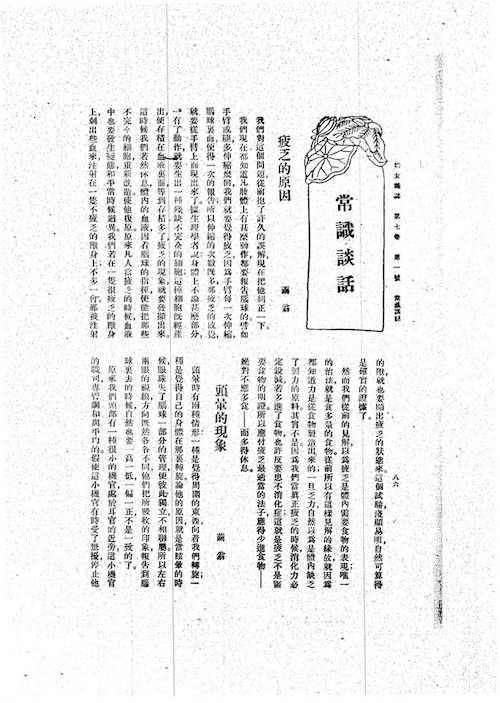
\includegraphics[width=\linewidth]{./figures/testset/02.jpg}
        \caption{02}
        \label{fig:test_02}
    \end{subfigure}
    \hfill
    \begin{subfigure}[b]{0.23\linewidth}
        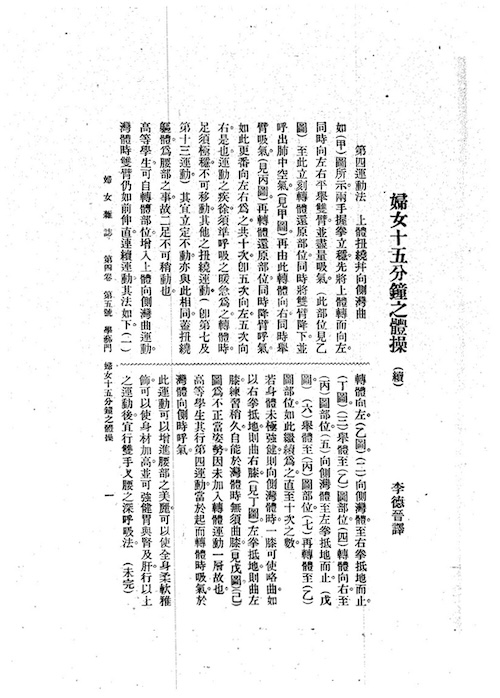
\includegraphics[width=\linewidth]{./figures/testset/03.jpg}
        \caption{03}
        \label{fig:test_03}
    \end{subfigure}
    \hfill
    \begin{subfigure}[b]{0.23\linewidth}
        \includegraphics[width=\linewidth]{./figures/testset/04.jpg}
        \caption{04}
        \label{fig:test_04}
    \end{subfigure}
  
    \begin{subfigure}[b]{0.23\linewidth}
        \includegraphics[width=\linewidth]{./figures/testset/05.jpg}
        \caption{05}
        \label{fig:test_05}
    \end{subfigure}
    \hfill
    \begin{subfigure}[b]{0.23\linewidth}
        \includegraphics[width=\linewidth]{./figures/testset/06.jpg}
        \caption{06}
        \label{fig:test_06}
    \end{subfigure}
    \hfill
    \begin{subfigure}[b]{0.23\linewidth}
        \includegraphics[width=\linewidth]{./figures/testset/07.jpg}
        \caption{07}
        \label{fig:test_07}
    \end{subfigure}
    \hfill
    \begin{subfigure}[b]{0.23\linewidth}
        \includegraphics[width=\linewidth]{./figures/testset/08.jpg}
        \caption{08}
        \label{fig:test_08}
    \end{subfigure}
    \caption{Test images 01 to 08}
    \label{fig:test_01_08}
\end{figure}

\begin{figure}[htbp]
    \centering
    \begin{subfigure}[b]{0.23\linewidth}
        \includegraphics[width=\linewidth]{./figures/testset/09.jpg}
        \caption{09}
        \label{fig:test_09}
    \end{subfigure}
    \hfill
    \begin{subfigure}[b]{0.23\linewidth}
        \includegraphics[width=\linewidth]{./figures/testset/10.jpg}
        \caption{10}
        \label{fig:test_10}
    \end{subfigure}
    \hfill
    \begin{subfigure}[b]{0.23\linewidth}
        \includegraphics[width=\linewidth]{./figures/testset/11.jpg}
        \caption{11}
        \label{fig:test_11}
    \end{subfigure}
    \hfill
    \begin{subfigure}[b]{0.23\linewidth}
        \includegraphics[width=\linewidth]{./figures/testset/12.jpg}
        \caption{12}
        \label{fig:test_12}
    \end{subfigure}
  
    \begin{subfigure}[b]{0.23\linewidth}
        \includegraphics[width=\linewidth]{./figures/testset/13.jpg}
        \caption{13}
        \label{fig:test_13}
    \end{subfigure}
    \hfill
    \begin{subfigure}[b]{0.23\linewidth}
        \includegraphics[width=\linewidth]{./figures/testset/14.jpg}
        \caption{14}
        \label{fig:test_14}
    \end{subfigure}
    \hfill
    \begin{subfigure}[b]{0.23\linewidth}
        \includegraphics[width=\linewidth]{./figures/testset/15.jpg}
        \caption{15}
        \label{fig:test_15}
    \end{subfigure}
    \hfill
    \begin{subfigure}[b]{0.23\linewidth}
        \includegraphics[width=\linewidth]{./figures/testset/16.jpg}
        \caption{16}
        \label{fig:test_16}
    \end{subfigure}

    \begin{subfigure}[b]{0.23\linewidth}
        \includegraphics[width=\linewidth]{./figures/testset/17.jpg}
        \caption{17}
        \label{fig:test_17}
    \end{subfigure}
    \hfill
    \begin{subfigure}[b]{0.23\linewidth}
        \includegraphics[width=\linewidth]{./figures/testset/18.jpg}
        \caption{18}
        \label{fig:test_18}
    \end{subfigure}
    \hfill
    \begin{subfigure}[b]{0.23\linewidth}
        \includegraphics[width=\linewidth]{./figures/testset/19.jpg}
        \caption{19}
        \label{fig:test_19}
    \end{subfigure}
    \hfill
    \begin{subfigure}[b]{0.23\linewidth}
        \includegraphics[width=\linewidth]{./figures/testset/20.jpg}
        \caption{20}
        \label{fig:test_20}
    \end{subfigure}
    \caption{Test images 09 to 20}
    \label{fig:test_09_20}
\end{figure}

\end{appendices}
%%%%%%%%%%%%%%%%%%%%%%%%%%%%%%%%%%%%

%% bibliography
\bibliographystyle{vancouver}
\bibliography{reference}

\end{document}
